%%%%%%%%%%%%%%%%%%%%%%%%%%%%%%%%%%%%%%%%%%%%%%%%%%%
%% LaTeX book template                           %%
%% Author:  Amber Jain (http://amberj.devio.us/) %%
%% License: ISC license                          %%
%%%%%%%%%%%%%%%%%%%%%%%%%%%%%%%%%%%%%%%%%%%%%%%%%%%
%!TEX TS-program = pdfLaTeX
%!TEX encoding = utf-8
%!TEX spellcheck = fr-FR

\documentclass[12pt,twoside,openright]{book}

%\usepackage{soul}

%\documentclass[a4paper,11pt]{book}
\usepackage[T1]{fontenc}
\usepackage[utf8]{inputenc}
\usepackage[francais]{babel}

\usepackage[usenames,dvipsnames]{color}

\usepackage{lmodern}
%%%%%%%%%%%%%%%%%%%%%%%%%%%%%%%%%%%%%%%%%%%%%%%%%%%%%%%%%
% Source: http://en.wikibooks.org/wiki/LaTeX/Hyperlinks %
%%%%%%%%%%%%%%%%%%%%%%%%%%%%%%%%%%%%%%%%%%%%%%%%%%%%%%%%%
\usepackage{hyperref}
\usepackage{graphicx}
\usepackage{pdfpages}
\usepackage{amsmath}
\usepackage{amssymb}
\usepackage{a4}
\usepackage{indentfirst}
\usepackage{fancyhdr}
\usepackage{varioref}
\usepackage{makeidx}

\usepackage{mslapa}

\usepackage{ulem}

%\usepackage{apacite}
%\usepackage[longnamesfirst,nonamebreak]{natbib}




%%%%%%%%%%%%%%%%%%%%%%%%%%%%%%%%%%%%%%%%%%%%%%%%%%%%%%%%%%%%%%%%%%%%%%%%%%%%%%
%%%%%%%%%%%%%%%%%%%%%%%%%%%%%%%%%%%%%%%%%%%%%%%%%%%%%%%%%%%%%%%%%%%%%%%%%%%%%%

\pagestyle{fancy}

\addtolength{\headwidth}{\marginparsep}
\addtolength{\headwidth}{\marginparwidth}
\renewcommand{\chaptermark}[1]{\markboth{#1}{}}
\renewcommand{\sectionmark}[1]{\markright{\thesection\ #1}}
\fancyhf{}
\fancyhead[LE,RO]{\bfseries\thepage}
\fancyhead[LO]{\bfseries\rightmark}
\fancyhead[RE]{\bfseries\leftmark}
\fancypagestyle{plain}{
\fancyhead{} % get rid of headers
\renewcommand{\headrulewidth}{0pt} % and the line
}


%% Apalike hyphenation %%%
%\let\oldbibitem=\bibitem
%\renewcommand{\bibitem}[2][]{\oldbibitem[#1]{#2}\newline}

%%% Margins %%%
\voffset -1.04cm
\textheight 23cm
\hoffset -1in
\evensidemargin 2.5cm
\oddsidemargin 2.5cm
\textwidth 16cm

%%%%%%%%%%%%%%%%%%%%%%%%%%%%%%%%%%%%%%%%%%%%%%%%%%%%%%%%%%%%%%%%%%%%%%%%%%%%%%
%%%%%%%%%%%%%%%%%%%%%%%%%%%%%%%%%%%%%%%%%%%%%%%%%%%%%%%%%%%%%%%%%%%%%%%%%%%%%%

%\textwidth16cm
%\textheight23cm
%\oddsidemargin0,5cm
%\evensidemargin0,5cm
%\topmargin-1cm
%\parskip0,5cm
%\parindent0cm



%%%%%%%%%%%%%%%%%%%%%%%%%%%%%%%%%%%%%%%%%%%%%%%%%%%%%%%%%%%%%%%%%%%%%%%%%%%%%%%%
% 'dedication' environment: To add a dedication paragraph at the start of book %
% Source: http://www.tug.org/pipermail/texhax/2010-June/015184.html            %
%%%%%%%%%%%%%%%%%%%%%%%%%%%%%%%%%%%%%%%%%%%%%%%%%%%%%%%%%%%%%%%%%%%%%%%%%%%%%%%%
\newenvironment{dedication}
{
   \cleardoublepage
   \thispagestyle{empty}
   \vspace*{\stretch{1}}
   \hfill\begin{minipage}[t]{0.66\textwidth}
   \raggedright
}
{
   \end{minipage}
   \vspace*{\stretch{3}}
   \clearpage
}

%%%%%%%%%%%%%%%%%%%%%%%%%%%%%%%%%%%%%%%%%%%%%%%%
% Chapter quote at the start of chapter        %
% Source: http://tex.stackexchange.com/a/53380 %
%%%%%%%%%%%%%%%%%%%%%%%%%%%%%%%%%%%%%%%%%%%%%%%%
\makeatletter
\renewcommand{\@chapapp}{}% Not necessary...
\newenvironment{chapquote}[2][2em]
  {\setlength{\@tempdima}{#1}%
   \def\chapquote@author{#2}%
   \parshape 1 \@tempdima \dimexpr\textwidth-2\@tempdima\relax%
   \itshape}
  {\par\normalfont\hfill--\ \chapquote@author\hspace*{\@tempdima}\par\bigskip}
\makeatother


% Babel ``Sommaire'' à la place de ``table des matières''
\renewcommand{\contentsname}{Sommaire}


%%%%%%%%%%%%%%%%%%%%%%%%%%%%%%%%%%%%%%%%%%%%%%%%%%%
% First page of book which contains 'stuff' like: %
%  - Book title, subtitle                         %
%  - Book author name                             %
%%%%%%%%%%%%%%%%%%%%%%%%%%%%%%%%%%%%%%%%%%%%%%%%%%%

% Book's title and subtitle
\title{\Huge \textbf{Apprentissage dans les architectures cognitives}  \\ \vspace{1cm} \huge Contributions pour l'informatique et les neurosciences \\ \vspace{1cm}}
% Author
\author{\textsc{Emmanuel Daucé}}%\thanks{\url{www.example.com}}}


\begin{document}

\frontmatter
\maketitle

%%%%%%%%%%%%%%%%%%%%%%%%%%%%%%%%%%%%%%%%%%%%%%%%%%%%%%%%%%%%%%%
% Add a dedication paragraph to dedicate your book to someone %
%%%%%%%%%%%%%%%%%%%%%%%%%%%%%%%%%%%%%%%%%%%%%%%%%%%%%%%%%%%%%%%
%\begin{dedication}
%Dedicated to Calvin and Hobbes.
%\end{dedication}

%%%%%%%%%%%%%%%%%%%%%%%%%%%%%%%%%%%%%%%%%%%%%%%%%%%%%%%%%%%%%%%%%%%%%%%%
% Auto-generated table of contents, list of figures and list of tables %
%%%%%%%%%%%%%%%%%%%%%%%%%%%%%%%%%%%%%%%%%%%%%%%%%%%%%%%%%%%%%%%%%%%%%%%%
\tableofcontents
%\listoffigures
%\listoftables

\mainmatter

%\section*{Remerciements}
%\begin{itemize}
%\item A special word of thanks goes to Professor Don Knuth\footnote{\url{http://www-cs-faculty.stanford.edu/~uno/}} (for \TeX{}) and Leslie Lamport\footnote{\url{http://www.lamport.org/}} (for \LaTeX{}).
%\item I'll also like to thank Gummi\footnote{\url{http://gummi.midnightcoding.org/}} developers and LaTeXila\footnote{\url{http://projects.gnome.org/latexila/}} development team for their awesome \LaTeX{} editors.
%\item I'm deeply indebted my parents, colleagues and friends for their support and encouragement.
%\end{itemize}
%\mbox{}\\
%\mbox{}\\
%\noindent Amber Jain \\
%\noindent \url{http://amberj.devio.us/}

%%%%%%%%%%%%%%%%
% NEW CHAPTER! %
%%%%%%%%%%%%%%%%


%%%%%%%%%%%%%%%%%%%%%%%%%%%%%%%%%%%%%%%%%%%%%%%%%%%%%%%%%%%%%%%%%%%%%%%%%%%%%%%%%%%%%%%%%%%%%%%%%%%%%%%%%%%%%%%%%11
%%%%%%%%%%%%%%%%%%%%%%%%%%%%%%%%%%%%%%%%%%%%%%%%%%%%%%%%%%%%%%%%%%%%%%%%%%%%%%%%%%%%%%%%%%%%%%%%%%%%%%%%%%%%%%%%%%%
%%%%%%%%%%%%%%%%%%%%%%%%%%%%%%%%%%%%%%%%%%%%%%%%%%%%%%%%%%%%%%%%%%%%%%%%%%%%%%%%%%%%%%%%%%%%%%%%%%%%%%%%%%%%%%%%%%%
%%%                                            ##                                                               %%% 
%%%                                          ####                                                               %%%  
%%%                                            ##                                                               %%% 
%%%                                            ##                                                               %%% 
%%%                                            ##                                                               %%%    
%%%                                            ##                                                               %%% 
%%%                                          ######                                                             %%% 
%%%%%%%%%%%%%%%%%%%%%%%%%%%%%%%%%%%%%%%%%%%%%%%%%%%%%%%%%%%%%%%%%%%%%%%%%%%%%%%%%%%%%%%%%%%%%%%%%%%%%%%%%%%%%%%%%%%
%%%%%%%%%%%%%%%%%%%%%%%%%%%%%%%%%%%%%%%%%%%%%%%%%%%%%%%%%%%%%%%%%%%%%%%%%%%%%%%%%%%%%%%%%%%%%%%%%%%%%%%%%%%%%%%%%%%
%%%%%%%%%%%%%%%%%%%%%%%%%%%%%%%%%%%%%%%%%%%%%%%%%%%%%%%%%%%%%%%%%%%%%%%%%%%%%%%%%%%%%%%%%%%%%%%%%%%%%%%%%%%%%%%%%%%


\chapter{Introduction}


%%%%%%%%%%%%%%%%%%%%%%%%%%%%%%%%%%%%%%%%%%%%%%%%%%%%%%%%%%%%%%%%%%%%%%%%%%%%%%%%%%%%%%%%%%%%%%%%%%%%%%%%%%%%%%%%%%%
%%%%%%%%%%%%%%%%%%%%%%%%%%%%%%%%%%%%%%%%%%%%%%%%%%%%%%%%%%%%%%%%%%%%%%%%%%%%%%%%%%%%%%%%%%%%%%%%%%%%%%%%%%%%%%%%%%%
%%%%%%%%%%%%%%%%%%%%%%%%%%%%%%%%%%%%%%%%%%%%%%%%%%%%%%%%%%%%%%%%%%%%%%%%%%%%%%%%%%%%%%%%%%%%%%%%%%%%%%%%%%%%%%%%%%%
%%%%%%%%%%%%%%%%%%%%%%%%%%%%%%%%%%%%%%%%%%%%%%%%%%%%%%%%%%%%%%%%%%%%%%%%%%%%%%%%%%%%%%%%%%%%%%%%%%%%%%%%%%%%%%%%%%%
%%%%%%%%%%%%%%%%%%%%%%%%%%%%%%%%%%%%%%%%%%%%%%%%%%%%%%%%%%%%%%%%%%%%%%%%%%%%%%%%%%%%%%%%%%%%%%%%%%%%%%%%%%%%%%%%%%%
%%%%%%%%%%%%%%%%%%%%%%%%%%%%%%%%%%%%%%%%%%%%%%%%%%%%%%%%%%%%%%%%%%%%%%%%%%%%%%%%%%%%%%%%%%%%%%%%%%%%%%%%%%%%%%%%%%%



%\begin{chapquote}{Author's name, \textit{Source of this quote}}
%``This is a quote and I don't know who said this.''
%\end{chapquote}

% le modèle de Hopfield
% Qu'est-ce que le chaos?

% Qu'est-ce qu'un système apprenant

Le but de ce document est de fournir un aperçu étendu des questions et des approches que j'ai 
eu l'occasion d'aborder au cours des vingts dernières années, depuis mes premiers pas en recherche. 
{\color{Orange} Ce document est organisé autour des différentes contributions et productions scientifiques auxquelles
j'ai participé, dans un ordre non chronologique mais thématique.
A l'issue de ce parcours, il fournit également un aperçu d'un certain nombre de questions 
restées ouvertes, et pouvant faire l'objet de développements futurs.}

Ces différentes contributions appartiennent à un champ de recherche assez large à l'intersection
des neurosciences et de l'informatique, généralement appelé ``\textit{neurosciences computationnelles}''.
Le terme computationnel fait référence à la notion de calcul. On peut donc également parler de neuro-calcul,
bien que ce terme soit peu usité\footnote{  
sans doute pour ne pas le confondre avec le bio-calcul, 
qui concerne les opérations réalisées au niveau moléculaire, autrement dit
le fonctionnement de la cellule en tant que machine.}
\emph{Les neurosciences computationnelles 
visent donc à identifier ce qui, dans l'activité des neurones, s'apparente à un calcul; à identifier 
le type et la nature des opérations réalisées par le système nerveux}. 

{\color{Cyan}
Mon parcours en résumé...

L'organisation du document...
}

\section{Neurosciences computationnelles}

Si les principes de fonctionnement élémentaires du système nerveux central (neurones, synapses) 
commencent à être bien connus, 
le fonctionnement intégré du système dans son ensemble reste l'objet de nombreuses conjectures.
Les modèles mathématiques et les simulations informatiques permettent de proposer des hypothèses 
de fonctionnement et/ou 
de valider certaines hypothèses issues de l'observation. 
{\color{Orange} Les neurosciences computationnelles sont ainsi la branche de l'{\bf !!informatique!!} qui, d'une part, élabore des modèles de calcul 
	inspirés par les hypothèses proposées en neurosciences, et, d'autre part, propose des interprétations
	de données biologiques à partir de principes et modèles issus des sciences de l'information.}
Ainsi, l'étude du système nerveux, sous l'angle computationnel, a deux objectifs:
\begin{enumerate} 
\item explorer des mécanismes de calcul alternatifs 
\item comprendre le fonctionnement du cerveau
\end{enumerate}

\paragraph{Mécanismes de calcul alternatifs} Le premier objectif est
de s'inspirer du fonctionnement du système nerveux pour découvrir de nouveaux principes pour le calcul artificiel,
ou de nouvelles architectures, pour résoudre des problèmes qui résistent encore aux calculateurs actuels.
Mieux comprendre le cerveau, c'est donc potentiellement étendre le domaine de la science informatique,
étendre le type de données qu'elles sont capables de traiter (son, langage, images, ...), 
augmenter leur capacité à contrôler leur environnement, 
les rendre plus proches, 
en terme de fonctionnement, des humains avec lesquels elles interagissent. 

\paragraph{Fonctionnement du cerveau} Le deuxième objectif consiste 
à utiliser les connaissance informatiques et mathématiques actuelles pour mieux comprendre le système nerveux.
Il s'agit d'une certaine façon d'identifier ce qui dans l'activité nerveuse s'apparente aux algorithmes
utilisés dans des tâches computationnelles variées, comme le contrôle, l'apprentissage, le traitement des images et des données;
voir si les solutions mises au point dans des contextes d'ingénierie proches de celui face auquel se trouve
le système nerveux ont des équivalents au sein de l'activité nerveuse (ou si, au contraire, la nature 
utilise des principes et méthodes différents). L'objectif est, à partir des observations, de mieux 
identifier les rôles et les interactions à l'intérieur du système nerveux, et potentiellement
de mieux soigner les désordres et maladies neurologiques. 

{\color{Orange} Cette approche a environ une soixantaine d'années d'existence, {\bf !!!FLOU!!!et se confond parfois avec} 
les sciences cognitives
(étude des opérations de haut niveau réalisées par le cerveau), 
les neurosciences fonctionnelles (étude des rôles des différentes structures anatomiques), 
et l'apprentissage automatique (programmes s'adaptant aux données).}

{\color{Orange} Dans le cadre des neurosciences computationnelles, la question n'est pas nécessairement de
produire le meilleur algorithme, ou de résoudre une nouvelle tâche, mais de produire des
modèles permettant de mieux comprendre les opérations réalisées par le cerveau, ou de prendre
exemple sur des architectures ou des circuits neuronaux réels pour valider ou invalider des hypothèses
liées aux types d'opérations produites par le système nerveux.}



\subsection{Une nouvelle discipline?}



{\color{Purple} 
Les neurosciences computationnelles sont par définition pluridisciplinaires. 
\begin{itemize}
\item Elles reposent en premier lieu sur le 
champ des \textit{neurosciences}, qui ont connu un développement considérables au cours des quarante dernières années,
avec l'apparition de nouvelles techniques de mesure permettant d'observer le cerveau en fonctionnement à
différentes échelles. 
\item Elles reposent en second lieu sur la \textit{modélisation mathématique et informatique}, qui a également
connu un développement important lié à l'augmentation des capacités de calcul des ordinateurs, ainsi que de la
capacité à traiter des données massives à travers des techniques dites d'apprentisage automatique (\textit{Machine 
learning}). 
\item Un dernier champ de recherche, celui de la \textit{robotique autonome} et du contrôle moteur, est également impliqué, dans la mesure où le
développement d'interfaces bioniques nécessite une meilleure connaissance des mécanismes de 
contrôle à l'oeuvre chez l'homme et l'animal.
\end{itemize}
}

\paragraph{Trois niveaux d'analyse}
Selon la typologie classique proposée par David Marr \shortcite{Marr82}, 
un modèle peut appartenir à différents niveaux de généralité, à savoir le niveau computationnel (la 
logique), 
le niveau algorithmique (encodage et opérations réalisées), et
la réalisation matérielle (le réseau de neurones ou ``substrat'').   

Cette distinction en trois niveaux permet principalement de distinguer ce qui relève de la définition du problème~:
définition de la tâche, en fonction des contraintes physiques et de l'appareillage sensoriel et moteur, d'une part, et
d'autre part ce qui relève de la réalisation (algorithmique) de la tâche, c'est à dire principalement le circuit de 
traitement. C'est, en terminologie informatique, la distinction entre
l'équation à résoudre, la brique logicielle qui la résout et le circuit logique qui l'implémente.
Marr postule une relative indépendance entre les différents niveaux de description, en établissant une
claire séparation entre le substrat neuronal, le circuit de traitement et l'espace de la tâche. 

{\color{Orange}{\bf !!
	Cette séparation correspond assez bien au problème des disparités d'échelle 
	évoqué plus haut.!!} La contrainte physique du corps, engagé dans différentes tâches, à des échelles
spatiales macroscopiques et des échelles temporelles lentes d'une part.
La contrainte du circuit microscopique, constitué d'unité neuronales échangeant rapidement des signaux discrets
d'autre part.
Entre les deux, un niveau architectural, constitué de circuits imbriqués intégrant l'activité de
larges portion du cerveau, 
constituant un niveau de description relativement indépendant des deux autres.}

%XXXXXXXXXXXXXXXXXXXXXXXXXXXXXXXXXXXXXXXXXXXXXXXXXXXXXXXXXXXXXXXXXXXXXX
\paragraph{Approche ascendante (ou ``bottom-up'')}
La méthodologie ``bottom-up'' consiste à étudier les
\emph{conditions d'émergence} de fonctions de haut niveau à partir 
des caractéristiques d'un réseau de neurones plongé dans un
environnement contraignant.
Les réseaux de neurones sont en effet capables de manifester des formes d'organisation spontanée~: comportement critique, 
transitions entre différentes configurations d'activité, activité persistante et mémoire 
à court terme (rémanence) etc.
L'ajout de mécanismes de plasticité synaptique vise à exploiter 
cette richesse intrinsèque 
pour que le réseau puisse acquérir des connaissances et des compétences nouvelles.
{\color{Purple} 
A partir des constituants de la dynamique, de leurs propriétés (leur ``expressivité'') cette approche vise à 
établir les propriétés ou les fonctions qui peuvent être attendues de l'assemblage des constituants, autrement dit établir la 
``puissance'' d'un langage qui utiliserait 
l'activité des neurones comme syntaxe de base.
}

\paragraph{Approche descendance (ou ``top-down'')}
La méthodologie ``top-down'' consiste à étudier les \emph{conditions de réalisation}
d'une certaine tâche par étapes descendantes, de la contrainte générale du corps engagé dans la tâche
à la réalisation matérielle du circuit qui la résout.
L'approche descendante consiste souvent à identifier les aspects non-triviaux
d'une tâche. L'étude des temps de réponse, des courbes d'apprentissage et des
taux d'erreur permet d'explorer les caractéristiques limites d'un comportement et de mieux appréhender
les contraintes posées par système qui l'implémente physiquement.
Ce peuvent être des contraintes physiques (limites d'extension, de course, ...) mais
également des limites provenant des caractéristiques physiques du réseau de neurones sous-jacent.
L'élaboration d'un modèle descriptif prenant en compte plusieurs échelles permet alors d'émettre des hypothèses 
sur les sources (physiques ou logiques) des limitations comportementales observées. 

{\color{Violet}
\subsection{Développement}
Les neurosciences computationnelles se sont fortement développées, et ont commencé à
s'organiser en tant que champ de recherche, à partir de la fin des années 90, avec le soutien de plusieurs programmes 
nationaux et internationaux. On citera, parmi les plus actifs, le réseau
Bernstein pour les neurosciences computationnelles en Allemagne, développé depuis 2004, 
le collectif INSC (International Neuroinformatics Coordination Facility) qui tente de coordonner les 
nombreux projets de recherche de la discipline au niveau international (basé en Suède). Elles ont 
bénéficié de nombreux soutiens financiers européens (NEST, Brain scales, Blue Brain project, ...)
qui se sont récemment concrétisés par l'attribution d'un financement 'Flagship' pour le projet ``Human Brain
Project''  qui regroupe les principaux acteurs des projets précédents. 
Ce champ de recherche commence également à s'insérer dans les programmes de deuxième cycle, comme le montrent les
nombreux cours en ligne disponibles sur le Web
(voir par exemple ceux de Sébastien Seung au MIT, Andrew Ng à l'Université de Washington, etc.)

Au niveau des revues scientifiques, les neurosciences computationnelles ne bénéficient pas de la même
couverture académique que les disciplines plus anciennement implantées. 
Les revues qui ont historiquement participé à son développement sont les revues traitant des 
réseaux de neurones artificiels apparues à la fin des années 80 (Neural Networks, Neural 
Computation, Neural Computing Letters, Biogical Cybernetics, etc.).
Certaine revues plutôt dédiées au traitement du signal, comme Neuroimage, acceptent également des papiers du domaine.
Enfin, les revues de physique (Physica-D) hébergent également des papiers traitant des neurosciences computationnelles.  
Suite au développement du champ de recherche et de sa couverture relativement lacunaire par les revues scientifiques, 
sont apparues des revues en ``Open Acces'' spécialement dédiées au domaine. 
On notera en particulier PLOS-Computational Biology et Frontiers in Computational Neurosciences qui ont aidé à compenser
la relatif manque de visibilité du domaine.
Il existe enfin quelques conférences spécifiquement dédiées à ce champ de recherche, comme la conférence CNS (Computational
Neurosciences) et la conférence CoSyNe (Computational and Systems Neuroscience). Dans le domaine de la robotique bio-inspirée,
on peut citer la conférence SAB (Simulation of Adaptive Behavior) qui a eu un fort impact au début des années 2000 mais a 
fini par disparaître faute d'audience suffisante. 

\subsection{Les neurosciences computationnelles en France}
%Voir : https://web.archive.org/web/20131020013653/http://neurocomp.fr/

\subsection{Etat de l'art} Le champ de recherche s'organise autour de plusieurs pôles. 
(1) simulation neuro-réaliste : mieux comprendre le fonctionnement du neurone, et des interacions entre neurones. 
se cantonne parfois au simple neurone, à la stucture de la cellule. Modèles de plasticité synaptique, de la transmission
du signal nerveux, des échanges avec le milieu... (2) modèles conceptuels, principes de traitement de l'information,
codes neuronaux, mécanismes de mémoire et d'apprentissage;
(3) architectures neuronales, dynamique à large échelle, neurones à spikes, réseaux équilibrés (plutôt physique
théorique)...

Les principales avancées sont:
\begin{itemize}
 \item le système Visuel, Olshausen, les champs récepteurs, les architectures profondes, approche profonde; non-negative matrix factorization [LEE + SEUNG 1999].
 \item dynamique stochastique, Fokker-Planck, etats de haute conductance, réseaux équilibrés
 \item généralisation des modèles physiques à l'analyse de l'imagerie... Modèles inverses. Friston
 \item STDP et codage par rang
 \item modèles de la décision et circuit de la récompense. Modèles du cervelet. Kalman.
 \item ce qui se fait en robotique. Franceschini. Japonais. Peters. MIT.
\end{itemize}


Problèmes rencontrés : foisonnement des modèles et des simulateurs informatiques. Difficulté à  reproduire les résultats. 
problème de la validation des modèles. Confrontation aux données empiriques. 

Il manque : des principes fondateurs, un langage commun, 

\section{Parcours personnel} 


\subsection{Les années 90}

Les voies d'entrée dans cette branche de la recherche sont multiples, puisqu'on y trouve à la fois des mathématiciens, 
des informaticiens, des physiciens, des biologistes, des médecins et des psychologues. En ce qui me concerne, 
j'ai suivi un parcours classique d'élève-ingénieur via le système des classes préparatoires et 
des concours de Grandes Ecoles. J'ai intégré l'Ecole Nationale Supérieure d'Electronique, d'Electrotechnique, 
d'Informatique, d'Hydraulique de Toulouse (ENSEEIHT) en Septembre 2002. 

Ma spécialisation vers les sciences cognitives s'est  tout d'abord faite avec la rencontre en début de troisième année avec Bernard
Doyon, médecin et chercheur à l'INSERM (Hôpital de Purpan) suite aux assises du Pôle de Recherche en Science 
Cognitives de Toulouse (PRESCOT), tenues à Labège, les 23 et 24 
septembre 1994. Bernard Doyon y présentait  l'étude de comportements chaotiques
obtenus par simulation de réseaux de neurones, en faisant le parallèle avec le fonctionnement du cerveau 
(en particulier avec l'étude des dimensions fractales des signaux électrophysiologiques pour différents états de veille
et de sommeil, développée à l'époque par l'équipe d'Agnès Babloyantz à Bruxelles \shortcite{Bab85}, ainsi que les travaux
de Walter Freeman \shortcite{ska87} sur la réponse aus stimuli olfactifs sur des grilles d'électrodes chez le lapin).

Suite à une discussion, j'ai décidé de m'engager dans cette voie de recherche (simulation de réseaux de neurones
chaotiques) dans le cadre d'un stage du DEA de Representation de la Connaissance et Formalisation
du Raisonnement (RCFR), qui faisait partie des DEAs pouvant être suivis en parallèle de la troisième année d'études. 
Les cours étaient centrés sur la logique formelle, en particulier les grammaires génératives, 
les systèmes experts, les modèles linguistiques et la théorie de jeux. Les réseaux de neurones y étaient très peu voire 
pas abordés. 

Le stage était situé au sein du Département d'Etudes et de Recherche en Informatique (DERI), 
dans un laboratoire de l'Office Nationale de Recherche d'Etudes et de Recherche Aérospoatiales (ONERA) rattaché à 
l'Ecole Nationale Supérieure de l'Aéronautique et de l'espace (Sup'Aéro). 
J'ai intégré le petit groupe animé par Manuel Samuelidès, professeur à Supaéro, et Bernard Doyon, chercheur
à l'INSERM, autour des réseaux de neurones récurrents à connectivité aléatoire. Cette étude avait démarré 
au début des années 90.

Les premières études sur ce  type de modèle avaient été faites par Sompolinsky \shortcite{Som88} sur un système dynamique continu. 
L'analyse d'une variante à temps
discret avait été proposée par Cessac et Samuelidès \shortcite{Ces94}. La démonstration de {\color{Orange} cette propriété (dite de ``chaos local'')} a été  
formellement achevée, dans le cas discret, par Moynot et Samuelides \shortcite{Moy00a} en 2000.

Lors de mon arrivée, deux étudiants venaient de passer leur thèse sur ce thème.
D'un côté, Bruno Cessac, diplômé en physique théorique de l'université Paul Sabatier, avait travaillé sur l'analyse en
champ moyen des réseaux de neurones récurrents aléatoires \cite{Ces95}. De l'autre, Mathias Quoy, diplômé de l'ENSEEIHT,
avait travaillé sur le comportement à taille finie (route vers le chaos) \cite{Doyon1993,CESSAC94}.
Mon rôle était alors principalement de continuer cette ligne de recherche,
et en particulier approfondir la question de la plasticité synaptique
et de l'apprentissage dans ce type de réseaux. 

Je connaissais alors peu de choses des systèmes dynamiques et du chaos, et mes connaissances en neurosciences se 
limitaient à une culture grand public, via quelques lectures. C'est donc principalement au travers 
de lectures de travaux scientifiques que je me suis formé à ces deux domaines.
L'ambiance de travail était très stimulante et nous avons rapidement pu produire 
de nouveaux résultats qui ont constitué mon rapport de fin d'études et de DEA \cite{Dau95}.
J'ai obtenu mon diplôme d'ingénieur informaticien en juin 1995 et mon diplôme de DEA en septembre 1995. 
Ayant terminé à la deuxième place, j'ai pu bénéficier d'une bourse ministérielle qui m'a permis de 
poursuivre en thèse, toujours sous la direction de Bernard Doyon, au sein de l'équipe animée par Manuel 
Samuelidès au DERI.

Le sujet étudié en DEA, n'ayant pas été épuisé, est donc devenu mon sujet de thèse. 
Plus précisément, ma thèse portait sur l'étude d'un mécanisme de \textit{réduction} de la dynamique
par plasticité synaptique au sein de réseaux de neurones récurrents aléatoires.
Il s'agissait d'un sujet assez vaste, qui s'est progressivement orienté vers 
l'apprentissage et la reconnaisssance de séquences spatio-temporelles dans les réseaux de neurones récurrents
organisés en plusieurs couches de traitement. 

Cette thèse m'a également permis d'assister à l'essor du champ des neurosciences computationnelles au cours des 
années 1995-2000  (sans directement
travailler sur ces sujets), avec (1) les premiers neurones à impulsions (Thorpe-DYNN-PCNN)
(2) l'émergence du concept de connectivté fonctionnelle large échelle
(3) les modèles de champ neuronaux (Schöner), les concepts de champ récepteur

Dans le même temps, le champ des réseaux de neurones artificiels se rapproche de plus en plus de l'apprentissage 
statistique (qui deviendra le ``Machine Learning'') avec l'essor des machines à vecteurs supports (SVM) à la fin des
années 90.

Les résultats de la thèse ont donné lieu à de nombreuses publications et présentations en conférences. 
premier papier qui présente ces idées de la manière la plus complète est celui de Neural Networks, 
datant de 1998 \shortcite{Dau98A} ({\bf !! VOIR... !!}).
Il porte sur l'étude de la réaction (spontanée ou acquise) d'un réseau de neurones récurrent aléatoire
à des patrons (stimuli) également aléatoires.

% 1999 - Moynot - Pinaud - Samuelides

Une partie du travail, portant sur des architectures
multi-couches, a été réalisé en collaboration avec Olivier Moynot, étudiant diplômé de l'ENS Cachan, qui a entamé 
sa thèse sous la direction de Manuel Samuelidès un an après moi, et Olivier Pinaud, étudiant en de DEA 
de physique théorique, qui a effectué son stage à l'ONERA au printemps 1998. 

{\color{Orange} En collaboration avec Olivier Moynot, Manuel Samuelides et Olivier Pinaud \shortcite{Dau99A,dauce01a}, j'ai également 
travaillé sur la définition et 
l'étude du comportement à taille finie d'un modèle de réseau de neurones aléatoire (RNA) multi-populations (voir section \ref{sec:balanced}).{\bf!! à développer!!}}

La troisième série de résultats de la thèse et des publication associées \shortcite{Dau00,Dau02} porte sur une architecture 
neuronale  permettant d'implémenter un modèle de la perception des signaux spatio-temporels.
Ces résultats reposent sur une architecture de réseaux récurrents aléatoires à plusieurs couches (deux ou trois).
Le formalisme multi-couches est le même que celui utilisé dans les réseaux équilibrés (voir section \ref{sec:balanced}).
Ici les couches se distinguent non par la nature de leurs neurones mais par le rôle qu'elles prennent dans le processus
d'apprentissage : une (ou deux) couche(s) primaire(s) ayant un rôle passif (sans dynamique intrinsèque)
et une couche secondaire (ou associative) possédant une dynamique intrinsèque, analogue aux réseaux récurents aléatoires
à une population.

L'étude du mécanisme de reconnaissance par ``réduction'' de la dynamique constitue le coeur
de ma thèse,



Varela : ``le monde visuel est constitué par l'action''

Sciences du sport : aproche écologique - Gibson. Biophysique.
La tradition biomécanique de Marseille.

Jirsa : école cybernétique 
}

  



Les recherches que j'ai menées balayent un grand nombre de modèles, des plus détaillés ({\bf !!REF!! neurones à 
impulsion} \cite{gerstner02}, {\bf !!REF!! neurones à conductance}) \cite{HH52} 
aux plus grossiers (activités de {\bf !!REF!! masses neuronales} à l'échelle
macroscopique \cite{Wilson1972}, modèles basés sur des mesures psychophysiques). 
Différentes architectures et méthodes d'apprentissage sont proposées, reposant sur différents 
paradigmes ({\bf !!supervisé} \cite{Rosen58}, {\bf !!REF!! non supervisé} \cite{Koh82}, 
{\bf !!REF!! par renforcement} \cite{SUTTON98}), 
sur des tâches de contrôle en boucle ouverte ou
en boucle fermée, et s'inspirant à des degrés divers de l'architecture du système nerveux.

{\color{Orange} Ce rapport {\bf!!évite les détails mathématiques!!}, et insiste sur la mise en perspectives des travaux présentés
dans le cadre des problématiques des neurosciences computationnelles. 
Pour les figures, formules et illustrations, il faudra se reporter au document annexe contenant  une sélection
de papiers et de contributions à des conférences scientifiques.}


%%% Ici on va expliquer le vocabulaire de base : les syst dynamiques, la plasticité, l'apprentissage, le contrôle
%%% en boucle fermée

Ce document est organisé en quatre grandes parties. 
\begin{itemize}
 \item Dynamique des grands réseaux de neurones aléatoires
 \item Plasticité synaptique et apprentissage
 \item Architectures de contrôle
 \item Projet scientifique
\end{itemize}

Les trois premières parties présentent les résultats  



%%%%%%%%%%%%%%%%%%%%%%%%%%%%%%%%%%%%%%%%%%%%%%%%%%%%%%%%%%%%%%%%%%%%%%%%%%%%%%%%%%%%%%%%%%%%%%%%%%%%%%%%%%%%%%%%%22
%%%%%%%%%%%%%%%%%%%%%%%%%%%%%%%%%%%%%%%%%%%%%%%%%%%%%%%%%%%%%%%%%%%%%%%%%%%%%%%%%%%%%%%%%%%%%%%%%%%%%%%%%%%%%%%%%%%
%%%%%%%%%%%%%%%%%%%%%%%%%%%%%%%%%%%%%%%%%%%%%%%%%%%%%%%%%%%%%%%%%%%%%%%%%%%%%%%%%%%%%%%%%%%%%%%%%%%%%%%%%%%%%%%%%%%
%%%                                                 #######                                                     %%%
%%%                                                ##     ##                                                    %%%    
%%%                                                       ##                                                    %%%     
%%%                                                 #######                                                     %%%   
%%%                                                ##                                                           %%%
%%%                                                ##                                                           %%% 
%%%                                                #########                                                    %%% 
%%%%%%%%%%%%%%%%%%%%%%%%%%%%%%%%%%%%%%%%%%%%%%%%%%%%%%%%%%%%%%%%%%%%%%%%%%%%%%%%%%%%%%%%%%%%%%%%%%%%%%%%%%%%%%%%%%%
%%%%%%%%%%%%%%%%%%%%%%%%%%%%%%%%%%%%%%%%%%%%%%%%%%%%%%%%%%%%%%%%%%%%%%%%%%%%%%%%%%%%%%%%%%%%%%%%%%%%%%%%%%%%%%%%%%%
%%%%%%%%%%%%%%%%%%%%%%%%%%%%%%%%%%%%%%%%%%%%%%%%%%%%%%%%%%%%%%%%%%%%%%%%%%%%%%%%%%%%%%%%%%%%%%%%%%%%%%%%%%%%%%%%%%%


\chapter{Dynamique des grands réseaux de neurones aléatoires}\label{chap:dyn}

{\color{Cyan} Ce chapitre est consacré à l'analyse des capacités d'expression des grands réseaux de neurones. Je présente dans une première section quelques notions essentielles concernant la modélisation des neurones et des réseaux de neurones. La deuxième section présente quelques notions plus spécifiques à l'étude des grands réseaux de neurones ainsi que des propositions propres à ce mémoire. Enfin, la troisième section présente quelques résultats issus des travaux auxquels j'ai participé dans ce cadre.  [REPRENDRE CHAPEAU]}

\cleardoublepage

\section{Notions générales}

Cette section présente un formalisme et des définitions visant à établir un cadre commun aux
études portant sur les ``réseaux de neurones''. 
La plupart des définitions sont donc extrêmement générales, avec un niveau de détail faible.
Les références et exemples indiqués permettent au lecteur d'approfondir les notions
présentées s'il le souhaite.

\subsection{Neurones et réseaux}

Inspirés par le fonctionnement du cerveau, les réseaux de neurones sont des modèles de calculateurs 
 dans lesquels le ``programme'' (la fonction de réponse) est décrite par un graphe.
Ce graphe est constitué d'un ensemble de nœuds, qui sont les unités de calcul, et un ensemble d'arêtes,  
pondérées et orientées, %définissant l'intensité du signal
qui transportent le signal entre les différentes unités de calcul.

Il existe de nombreux modèles de neurones et de nombreux modèles de réseaux de neurones. La modélisation des processus neuronaux
repose donc sur un choix du modélisateur, qui est fonction du mécanisme qu'il souhaite étudier, des outils
d'analyse et/ou de la puissance de calcul dont il dispose. 

Je liste ci-dessous quelques propriétés et éléments de vocabulaire communs à la plupart des modèles de réseaux de
neurones, indépendamment de leur utilisation en modélisation ou en apprentissage automatique. 

\subsubsection{Activité et signal}

Chaque unité de calcul (ou neurone) est modélisée comme une fonction de réponse $f$ qui 
traite un jeu de \textit{données d'entrée} multimodal $s^\text{in}_1, ..., s^\text{in}_n$.
On peut supposer sans perte de généralité que les données d'entrée sont indexées sur l'axe temporel.
On parle alors de \textit{signal d'entrée} où $s^\text{in}_i = \{s^\text{in}_i(t)\}_{t \in \{t_0,... t_f\}}$ 
représente un jeu de données indexé sur une trame temporelle et 
$s^\text{in}_i(t)$ représente un point de mesure du $i^\text{ème}$ signal à l'instant $t$.

La sortie du neurone au temps $t_f$ est un scalaire: 
\begin{align}\label{eq:neurone_s_out}
s^\text{out}(t_f) = f(s^\text{in}_1, ..., s^\text{in}_n)
\end{align}
(on parle aussi de \textit{réponse} du neurone aux signaux d'entrée).
Un neurone est donc une unité élémentaire de traitement des données. %Un neurone est implicitement une unité de traitement \textit{non-linéaire}.

Le signal de sortie du neurone $s^\text{out} = \{s^\text{out}(t)\}_{t \in \{t_0,... t_f\}}$ est constituée 
d'une succession d'états ``hauts'' et d'états ``bas''.
Un neurone dont la sortie à l'instant $t$ est dans l'état haut est dit \textit{activé}. Un neurone 
dont la sortie à l'instant $t$ est dans l'état bas est dit \textit{inactif}. 

\emph{Exemples:}
\begin{itemize}
\item Dans le cas le plus simple des neurones binaires, 
le signal de sortie est une succession de 0 (inactif) ou de 1 (actif) \shortcite{MCu43}. 
\item Dans le cas plus complexe de neurones à impulsions, le signal de sortie est un train de potentiels d'action (PA), représenté par une 
somme de Diracs tels que $s(t) = \sum_{\hat{t} \in \mathcal{T}_\text{out}} \delta(t - \hat{t})$, où $\mathcal{T}_\text{out}$ est un ensemble
contenant les instants de décharge (voir par exemple \shortcite{gerstner02}).
%Dans le cas de neurones fréquentiels, le signal contient des grandeurs continues correspondant à la fréquence de décharge instantanée
%de la sortie.
\end{itemize}

Le signal de sortie (la suite d'états hauts et d'états bas) est aussi appelé l'\textit{activité} du neurone. Ce signal est transporté sur un axone, qui se
sépare à son extrémité en plusieurs branches se terminant par une (ou plusieurs) synapse(s). 

Les synapses sont les canaux d'entrée des neurones. 
Chaque synapse traite un signal $s_i^\text{in}$ émis par un autre neurone pré-synaptique $i$ du réseau et produit une \textit{entrée synaptique} $e(s_i^\text{in}$).
L'état \textit{interne} du neurone post-synaptique est donné par son \textit{potentiel de membrane} $V$.
La somme des entrées synaptiques agit sur la valeur de ce potentiel de membrane. 
L'intégration de la totalité des entrées peut être exprimée par une fonction de mise à jour du potentiel de membrane de la forme:
\begin{align}\label{eq:neurone_V}
V = g(s_1^\text{in}, ..., s_n^\text{in})
\end{align}
où $s_1^\text{in}, ..., s_n^\text{in}$ sont les $n$ signaux entrants.

\emph{Exemples:}
\begin{itemize}
\item Dans le cas le plus simple, $g$ est une combinaison linéaire des entrées synaptiques \shortcite{MCu43,Rosen58}.
\item Les modèles plus détaillés prennent en compte 
la fonction de transfert des synapses ainsi que les interactions non-linéaires entre les influences excitatrices et les influences inhibitrices \shortcite{DESTEXHE97}.
\end{itemize}

L'activation d'un neurone repose ensuite sur un mécanisme non linéaire de \textit{passage de seuil}.

\emph{Exemples:}
\begin{itemize}
\item Dans le modèle le plus simple \shortcite{MCu43}, l'état de sortie (0 ou 1) dépend d'un
seuil d'activation $\theta$ tel que $s=1$ (état haut) si $V>\theta$ et $s=0$ (état bas) sinon.
\item
Dans les modèles plus détaillés \shortcite{Lapicque1907,HH52}, le passage à l'état haut déclenche un mécanisme actif de réinitialisation qui ramène
le potentiel de membrane vers sa valeur de repos $V_0 < \theta$.  Ce mécanisme de réinitialisation, qui interdit
le maintien de la sortie dans l'état haut, rend l'état haut  
plus rare (et donc plus porteur d'information) que l'état bas. Il a également pour effet d'effacer 
la mémoire des données d'entrée antérieures au dernier potentiel d'action.
\end{itemize}


%% A mettre dans la partie sur la plasticité
%Un des modèles les plus étudiés en modélisation est le modèle de l'\textit{intégrateur à fuite}. 
%La valeur du potentiel dépend de l'historique des signaux d'entrée depuis le dernier PA jusqu'à l'instant $t$. 
%{\bf !! TODO  mécanisme de décision basé sur l'accumulation + figure!!}.
% La partie suivante doit commencer avec les modèles de la décision : décision bayésienne, intégrateur à seuil, décision de Hopfield,
% décision du champ neuronal, avec pour finir le modèle de Pouget (compromis dynamique)
% Préciser ensuite le mécanisme de sélection/intégration

\subsubsection{Réseau de neurones}

Plusieurs neurones connectés entre eux via des axones constituent 
un \textit{réseau de neurones}. Le schéma de connexion, sous la forme d'un graphe orienté, 
caractérise l'\textit{organisation structurelle} du réseau. 
%Selon que le graphe est acyclique, ou au contraire récurrent, .

La description du réseau est donné par une \textit{fonction de couplage},
définie le plus souvent par un tableau à double entrée noté $G$. Chaque neurone
se voit attribuer un indice $i \in 1,...,N$ où $N$ est le nombre de neurones dans le réseau. Le tableau
$G[i,j]$ contient alors les caractéristiques du lien du neurone $i$ vers le neurone $j$.
Un exemple de paramétrisation est le temps de propagation $\tau_{ij}$ et poids synaptique $J_{ij}$. 
Lorsque le poids synaptique est non-nul, on dit que les neurones $i$ et $j$ sont couplés. 
Si $N$ est le nombre de neurones, le nombre de paramètres du réseau est en $O(N^2)$, correspondant à un principe de transmission du signal \textit{de plusieurs à plusieurs} (un neurone envoie son signal de sortie vers plusieurs destinataires, un neurone reçoit des signaux de plusieurs émetteurs).

\emph{Notations:}
\begin{itemize} 
\item Le \textit{vecteur d'activité} $\boldsymbol{s}(t)$ (ou activité de population) est un vecteur de taille $n$ contenant l'ensemble des 
sorties à l'instant $t$~: 
$$\boldsymbol{s}(t) = (s_1^\text{out}(t), ..., s_n^\text{out}(t))$$
\item Le \textit{patron d'activité} est constituée de l'ensemble des signaux émis entre l'instant initial $t_0$  et l'instant d'observation $t$, soit: $$\boldsymbol{S}(t)=\{\boldsymbol{s}(t')\}_{t' \in [t_0, t[}$$
\end{itemize}

Les activités des différents neurones sont donc \textit{inter}dépendantes du fait des couplages. 
La \textit{fonction de réponse} du réseau $f$ est une fonction paramétrique 
décrite par le tableau de paramètres $G$, telle que l'activité $\boldsymbol{s}(t)$ est solution de~:
\begin{align}\label{eq:optim}
\boldsymbol{s}(t) = f(\boldsymbol{S}(t);G)
\end{align}
Il faut ici préciser, dans la mesure où les temps de transports sont supposés strictement positifs, que l'activité du réseau au temps $t$ est
dépendante de l'historique des activités précédent strictement 
l'instant $t$. L'activité d'un neurone post-synaptique $i$ au temps $t$ est dépendante des signaux pré-synaptiques
produits aux instants $t' < t$, en tenant compte du \textit{temps de transport} de ces signaux sur les axones. Plus précisément, si $j$ est le 
neurone pré-synaptique et $i$ le neurone post-synaptique, on a:
\begin{align}\label{eq:transport}
s^\text{in}_{ij}(t) = s^\text{out}_{j}(t - \tau_{ij})
\end{align}

\subsubsection{Architecture de réseau}

On parle d'\textit{architecture de réseau} pour décrire les propriétés générales du graphe.
L'architecture définit généralement le nombre de couches, le type de connexions de couche à couche, 
et éventuellement le nombre de neurones par couche.
Un exemple typique d'architecture est l'organisation séquentielle des réseaux de neurones dits
``à couche cachée'',
qu'on trouve dans les perceptrons multi-couches, les réseaux profonds, etc. [CITATIONS] 
Un autre exemple d'architecture est celle des mémoires associatives, constituées d'une ou plusieurs couches de 
neurones connectés sous la forme d'un circuit récurrent (ou réentrant) [CITATION].

{\color{Cyan} Notion de faisceau d'axones. Construction de réseaux.}

\subsubsection{Calcul distribué}

Les signaux transitant de neurone à neurone via les axones du réseau contiennent une succession d'états hauts et
d'états bas qui présentent une ressemblance  avec les signaux digitaux produits par les calculateurs 
numériques. Cette analogie de forme n'implique cependant pas que les principes de traitement et
de transformation de ces signaux soient les mêmes.

Du point de vue des calculateurs numériques, un calcul est décrit comme une séquence d'opérations élémentaires réalisées dans un certain ordre
à partir de données d'entrée. Ces opérations élémentaires peuvent être réalisées par les portes logiques
d'un circuit électronique, ou par tout mécanisme automatique capable de ségréguer ses entrées sous la forme d'au moins 
deux états de sortie distincts. 
%La généralisation 
%aux calculateurs universels se fait à travers la présence de mémoires, c'est à dire d'unités capables de
%conserver un état (haut ou bas) pour une durée indéterminée. 

Dans la cas des réseaux de neurones, la mise en œuvre d'un calcul repose sur la présence
de neurones d'\textit{entrée} soumis à des données extérieures, qui sont donc les opérandes du calcul.
C'est le cas chez l'animal des cellules \textit{sensorielles}. 
On note $\boldsymbol{I}(t) = \{\boldsymbol{I}(t')\}_{t' \in [t_0, t[}$ ce signal extérieur. 
Si le neurone $i$ est un neurone d'entrée, on a $I_i \neq 0$. Si le neurone $i$ n'est pas un neurone d'entrée,  
on a $I_i = 0$.
Le signal extérieur est généralement considéré comme indépendant de l'activité du réseau de neurones.

La \textit{réponse} du réseau de neurones au signal d'entrée (la solution du calcul) est le patron d'activité induit
 par ce signal d'entrée.
En étendant la fonction de réponse aux entrées extérieures, l'activité $\boldsymbol{s}(t)$ est la solution de~:
\begin{align}\label{eq:optim_input}
\boldsymbol{s}(t) = f(\boldsymbol{S}(t), \boldsymbol{I}(t);G)
\end{align}
On dit également 
que le réseau de neurones \textit{transforme} le signal d'entrée.

Il est possible de définir une \textit{fonction de sortie} qui \textit{décode} ce patron d'activité. 
La sortie du réseau est alors 
$$\boldsymbol{u} = h(\boldsymbol{s})$$
avec $h$ fonction de décodage (ou de ``\textit{read-out}'').

Plus globalement, la fonction d'entrée/sortie (fonction de transfert) du réseau de neurones est~:
\begin{align}\label{eq:E/S}
 \boldsymbol{u} = h(f(\boldsymbol{S},\boldsymbol{I};G))
\end{align}

La sortie $\boldsymbol{u}$ peut ainsi être interprétée comme le résultat du calcul réalisé à partir des données d'entrée $\boldsymbol{I}$. 
Dans la mesure où ce résultat est le produit de 
l'activité conjointe (et parallèle) des neurones du réseau, on se situe dans un contexte de \textit{calcul distribué}, par opposition au calcul
séquentiel centralisé réalisé par les ordinateurs traditionnels.



\subsection{Réseaux de neurones et modélisation biologique}

L'inspiration biologique conduit à étudier des modèles alternatifs au traitement
séquentiel standard. 
Dans le cadre de ce mémoire, nous regarderons en particulier 
l'idée de \textit{circuit reconfigurable}, basée sur l'existence d'une \textit{activité endogène} produite par un réseau de 
neurones \textit{récurrent}.  
Le but est de caractériser ces mécanismes, et 
d'identifier les points communs avec  
des mécanismes similaires à l'{\oe}uvre dans le cerveau. 

Les réseaux de neurones récurrents sont définis par le fait que leur graphe contient des cycles.
Ces cycles conduisent à des dépendances réciproques entre les unités du réseau. 
Le formalisme des systèmes dynamiques permet de décrire ces interactions croisées et leur effet sur les patrons
d'activité produits par le réseau.

\subsubsection{Quelques notions de la théorie des systèmes dynamiques}
L'activité du réseau au temps $t$ est le résultat de l'intégration des
potentiels d'action émis aux instants précédant $t$, en tenant compte des délais de transmission, et de la valeur courante du signal externe
(voir eq. (\ref{eq:optim_input})).

La théorie des \textit{systèmes dynamiques} repose sur un espace d'état $\mathcal{X}$, une trame temporelle 
$\mathcal{T}$ et un
flot $\phi$ qui est une application de $\mathcal{X} \times \mathcal{T}$ dans $\mathcal{X}$
définissant pour tout couple $(\boldsymbol{x},t)$ la valeur de l'état suivant:
\begin{align}\label{eq:SD}
\boldsymbol{x}' = \phi(\boldsymbol{x},t)
\end{align}
La plupart des réseaux de neurones peuvent se modéliser sous cette forme, à partir du moment où 
l'état du réseau à l'instant $t$ est entièrement spécifié, en tenant compte en particulier
du potentiel de membrane et 
des différents temps de transport sur les axones. 

La \textit{trajectoire} du système sur la plage temporelle $[t_0,t_f]$ est alors définie 
par l'intégration sur le flot de la condition initiale $\boldsymbol{x}_0$.

\begin{itemize}
\item Dans le cas d'un système dit ``autonome'', on a $\phi(\boldsymbol{x},t) = \phi(\boldsymbol{x})$ et
la trajectoire du système $\{\boldsymbol{x}(t)\}_{t \in [t_0,t_f], \boldsymbol{x}(t_0)= \boldsymbol{x}_0}$ 
est entièrement définie par les conditions initiales. 
\item Dans le cas d'un système dit ``ouvert'' (non-autonome), la dépendance temporelle
est souvent modélisée sous la forme d'un signal externe $\boldsymbol{I}(t)$, soit $\phi(\boldsymbol{x},t) = \phi(\boldsymbol{x},\boldsymbol{I}(t))$. 
Ce signal peut être:
  \begin{itemize}
  \item une donnée d'entrée dans le cas de modèles de traitement des données
  \item un bruit externe dans le cas de modèles stochastiques [REF?]
  \end{itemize}
\end{itemize}

{\color{Cyan}
Notions :
\begin{itemize}
 	\item notion de variable d'état définie pour tout $t$.
\end{itemize}
}

\paragraph{Systèmes dynamiques autonomes}
Dans le cas autonome...
{\color{Cyan} 

Notions :
\begin{itemize}
	\item système conservatif / dissipatif
	\item Notion d'attracteur =sous-ensemble connexe $C C \mathcal{X}$ invariant par le flot : $C = \phi(C)$.  Condition de stabilité différente si discret ou continu.
	\item relaxation du système (dynamique de relaxation). Différentes CI conduisent à différents attracteurs.
	\item paramètre de contrôle et bifurcations
	\item bassins d'attraction et séparatrices
	\item diagramme de phase
	\item paramètre d'ordre
\end{itemize}
}
\paragraph{Systèmes dynamiques ouverts}

Dans le cas non autonome, la trajectoire dépend à la fois des conditions initiales et du signal extérieur. 
\begin{itemize}
\item On parle dans ce cas d'une activité \textit{induite} par le signal d'entrée. 
\item Du point de vue 
computationnel, celà signifie que le même signal peut recevoir un traitement différent si les conditions initiales sont différentes. 
Sans précision des conditions initiales, de multiples opérations sont donc possibles pour un même signal d'entrée. 
{\color{Orange} On parlera de différents \textit{modes d'opération}}.
\end{itemize}


En pratique, l'équation (\ref{eq:SD}) prend souvent la forme d'une équation différentielle [REFS]
ou intégro-différentielle [REFS] qui se résout
par des méthodes numériques. 


%Dans un cadre continu, l'équation d'évolution est la suivante~:
%$$ \frac{d\boldsymbol{x}}{dt} = \Phi(\boldsymbol{x},t)$$
%Dans un cadre discret, l'équation d'évolution est~:
%$$ \boldsymbol{x}(t+1) = \Phi(\boldsymbol{x}(t),t)$$

%où $\Phi(\boldsymbol{x},t)$, où $t \in \mathcal{T}$ décrit un instant
%situé sur la trame temporelle et la variable d'état $\boldsymbol{x} \in \mathcal{X}$ décrit
%l'état du système.

\emph{Exemples:}
\begin{itemize}
\item Un exemple minimaliste est un réseau de neurones récurrent à deux neurones mutuellement connectés. 
Un tel réseau pourrait présenter deux modes : un mode ``inactif'' dans lequel les deux neurones
sont dans l'état ``bas'', et un mode ``actif'' dans lequel une activité ``haute'' locale est transmise
indéfiniment d'un neurone à l'autre. Chacun de ces deux patrons d'activité est une solution 
du graphe de contraintes. 
%\item 

\item {\color{Orange} L'exemple des réseaux de Hopfield \shortcite{Hop82} illustre bien la notion de modes multiples. 
%offre  un éclairage différent. 
%sur l'expressivité d'un substrat en mettant en 
%avant le caractère distribué (non-local) de l'activité. 
%Contrairement à l'idée classique d'un noeud de sortie comme unité d'expression, 
%(par exemple unité de séparation dans le cas des classifieurs, 
%unité de description dans le cas des cartes auto-organisées etc.), 
L'expressivité du réseau est vue sous l'angle du nombre
de patrons distribués (patterns) pouvant être obtenus en tant qu'état final (attracteur) atteint par le système
dynamique décrit par les poids (arêtes) du réseau.
La capacité s'exprime ici en nombre de \emph{modes} (configurations atteignables) 
et non en nombre de noeuds/vecteurs supports etc.
Si la capacité se trouve en principe augmentée
d'un facteur exponentiel ($2^N$ configurations distribuées possibles), 
la capacité effective est en pratique beaucoup plus réduite, 
se limitant à un nombre de modes (attracteurs) distincts en $O(N)$, 
c'est à dire de l'ordre du nombre de noeuds \shortcite{Amit1987,Tso88}.
La nature des opérations réalisables par le substrat est également différent puisqu'il s'agit principalement ici d'une
dynamique de relaxation adaptée à des opération de complétion et d'interpolation de données manquantes, implémentant un
mécanisme de mémoire dite ``auto-associative''. }
\item 

\end{itemize}


Lorsque le système est dissipatif, le flot définit un ensemble ... 

notion d'état du réseau, et de patron d'activité

axe temporel, système dynamique et conditions initiales.

équation d'évolution de la dynamique


Notions :
\begin{itemize}
 \item attracteur
 \item relaxation
 \item séparatrice
 \item paramètre de contrôle
 \item paramètre d'ordre
\end{itemize}


Dans le cadre des études inspirées par la biologie, il est fréquent d'utiliser des modèles plus simples
appelés modèles de \textit{champ moyen}.

Nous regardons en particulier le cas des réseaux de neurones 
récurrents aléatoires [A CONNECTER AU RESTE].

\subsubsection{Grands réseaux et champ moyen}


%Les modèle qui servent de fondement aux neurosciences computationnelles 
%sont les modèles de neurones à conductance [REF DESTEXHE] dont le plus connu est le modèle de Hudgkin-Huxley. 


\paragraph{Taux de décharge instantané} L'activité des neurones telle que mesurée par électrophysiologie présente
un caractère irrégulier où les temps d'émission des PA semblent obéir à un processus de Poisson [CITATION].
Un tel processus est caractérisé par sa fréquence instantanée $\nu$, qui donne le nombre de PA émis par seconde.
La grandeur $\nu$ peut être mesurée 
à travers l'observation d'un train de PA produit par un neurone particulier (nombre de PA émis divisé par
l'intervalle d'observation).

De nombreux modèles stochastiques de neurones ont été proposés qui prennent en compte le caractère aléatoire de la 
réponse des neurones biologiques. 


\paragraph{Activité de population}
Le modèle de champ moyen considère l'activité instantanée de populations de neurones $\nu(t)$, qui exprime, à un instant
donné, le nombre de neurones émettant un PA divisé par la taille de la population.
Un interprétation commune de l'activité des

\cleardoublepage

\section{Notions spécifiques et propositions}
Cette section 

{\color{Orange}
	\paragraph{!!Propositions!!}
	
	Il est souvent possible de regrouper différents patrons d'activité selon des caractéristiques communes
	se traduisant par une valeur unique au niveau de la fonction de sortie $h$. 
	\begin{itemize}
		\item On parlera des différents \textit{modes de sortie} du réseau de neurones.
		\item L'\textit{encodage} est le processus par lequel un jeu a priori non borné de signaux 
		d'entrée se traduira sous la forme d'un nombre fini de modes de sortie.
		Chaque mode est alors le reflet, au sein du réseau, d'une \textit{classe} de signaux. 
		\item On parlera d'\textit{expressivité} pour désigner le nombre et la nature des modes de sortie produits par un réseau de neurones,
		en présence ou en l'absence de signal extérieur. 
		Le nombre et la nature de ces modes
		nous permettra de décrire son ``vocabulaire'', ainsi que le type d'opérations dont il peut être le support. 
	\end{itemize}
	Notion de réponse d'un mode?  
}

{\color{Orange} Le fil rouge de notre approche} est celui des réseaux de neurones à connectivité aléatoire, 
permettant de traiter de manière formelle et de quantifier 
le caractère extrêmement inhomogène des réseaux de neurones naturels~: 
\begin{itemize}
	\item variété des types cellulaires, 
	\item variété des délais de
	transmission,
	\item variété de la forme et du nombre d'arborisations synaptiques,
	\item etc.
\end{itemize}

{\color{Orange} A travers l'analyse de la distribution des poids des connexions synaptiques
	%, de la distribution   leur intensité (?), 
	et de la distribution des délais associés,
	nous posons la question du rôle de ces distributions dans la formation de patrons d'activité (ou modes) variés, supports potentiels
	d'opérations cognitives. }

{\color{Cyan}{\bf
	Notion de répertoire dynamique =~ vocabulaire d'un langage =~ expressivité
	
	sec. 3.3.1 ~:}
	\begin{footnotesize}
    {\it 
	``Le changement observé suite à la présentation d'un stimulus statique ne correspond pas à 
	de la multistabilité au sens classique (un système dynamique multistable pouvant converger 
	vers différents attracteurs pour des conditions initiales différentes).
	Ici le stimulus fait partie des ``paramètres'' du
	réseau. Ainsi, chaque stimulus distinct définit système dynamique distinct 
	convergeant vers un attracteur distinct. 
	Le fait de modifier le stimulus au cours d'une même simulation 
	revient à modifier le système dynamique ``en cours de route''. 
	La réalisation d'une opération (sous la forme d'une réorganisation de la dynamique
	suite à l'imposition d'un motif statique) repose
	donc sur un mécanisme différent de celui proposé par Hopfield \shortcite{Hop82}.
	Il s'agit essentiellement d'une relaxation sous contrainte, chaque
	stimulus étant l'expression d'une contrainte différente.
	L'ensemble des réponses aux contraintes statiques possibles constitue le \textit{répertoire 
		dynamique} du réseau.
	}\end{footnotesize}''
	
	TODO~: tracer une analogie avec 
	\begin{itemize}
		\item les systèmes soumis à un signal variant au cours du temps $\rightarrow$ formalisme de Fokker-Planck
		\item les systèmes soumis à u bruit  
	\end{itemize}
}

\subsection{Grands réseaux de neurones aléatoires}

Un réseau de neurones aléatoire est un graphe orienté et pondéré $G$ constitué de $N$ nœuds défini par~:
\begin{itemize}
	\item la matrice des 
	couplages $\boldsymbol{J} = \{J_{i,j}\}_{i \in 1..N,j \in 1..N}$ 
	\item les seuils d'activation $\boldsymbol{\theta} = \{\theta_i\}_{i \in 1..N}$
	\item les temps de propagation  $\boldsymbol{\tau} = \{\tau_{i,j}\}_{i \in 1..N,j \in 1..N}$
	\item etc.
\end{itemize} 
tel que~:
\begin{align}
G \sim \mathcal{D}(\Theta)
\end{align}
où $\mathcal{D}$ est une distribution de probabilité sur l'espace des graphes et  $\Theta$ est un ensemble de paramètres qui définissent cette distribution.

L'ajout d'une fonction de réponse sur les nœuds définit un système dynamique déterministe, constitué de $N$ neurones.

La notion d'aléa ne porte donc pas sur la dynamique d'état mais sur le patron de connexions du réseau. 
On parle de bruit ``figé'' dans les connexions (``\textit{quenched disorder}'').


%Lorsque les liens $J_{ij}$ sont indépendants . 
L'indépendance entre les différents liens est une caractéristique importante, qui permet d'analyser le comportement du modèle 
à la limite des grandes tailles, c'est à dire en faisant tendre la taille $N$ vers l'infini. Avec un \textit{scaling} des poids approprié 
(espérance, variance de la loi de tirage initial des poids en $O(\frac{1}{N}$)), on peut montrer que la dynamique (déterministe) tend à la limite thermodynamique 
vers un processus aléatoire (processus Gaussien), la corrélation entre les nœuds tendant vers 0 \shortcite{Som88,Ces94,Moy00a}. 

%{\color{Violet} activité intrinsèque}

\subsubsection{Modèle à temps discret}

La dynamique à temps discret, et à temps de propagation constant est, en notation matricielle, définie par l'équation de récurrence ~:
\begin{align}
&\boldsymbol{x}(0) = \boldsymbol{x}_0&&\nonumber\\
&\forall t > 0 :&& \nonumber\\
&&\boldsymbol{h}(t) &= \boldsymbol{J} \mathbf{x}(t-1) - \boldsymbol{\theta}\\
&& \boldsymbol{x}(t) &= f(\boldsymbol{h}(t);g)\nonumber
\end{align}
avec $f$ fonction de réponse sigmoïde et $g$ paramètre de contrôle (gain de la fonction de réponse). 

\subsubsection{Limite thermodynamique}

 
Le comportement d'une classe de réseaux (l'ensemble des réseaux définis par la même distribution) peut être décrit à la limite thermodynamique par 
des équations dites de ``champ moyen''. Ces équations définissent le processus aléatoire limite, décrit par la dynamique temporelle de grandeurs caractéristiques comme l'activité moyenne, 
le moments d'ordre 2 et la covariance dans le temps \shortcite{Ces95}. 

Lorsque les poids synaptiques sont tirés indépendamment selon une loi de moyenne $\frac{\mu_J}{N}$ et d'écart-type $\frac{\sigma_J}{\sqrt{N}}$, et les seuils selon une loi de moyenne  $\mu_\theta$ et d'écart-type $\sigma_\theta$,
le processus Gaussien limite est défini au temps $t$ par~: 
\begin{itemize}
	\item sa moyenne $\mu_h(t) = \langle h_i(t)\rangle$
	\item sa variance $\sigma_h^2(t) = \langle (h_i(t) - \mu_h(t))^2\rangle$
	\item et sa covariance temporelle $\Delta_h(t,t') = \langle h_i(t) h_i(t') \rangle - \langle h_i(t) \rangle \langle h_i(t') \rangle$
\end{itemize}
où $h_i(t)$ est une variable aléatoire, selon:
\begin{align}
&\mu_h(t) = \mu_J m(t-1) + \mu_\theta\\
&\sigma_h^2(t) = \sigma_J^2 q(t-1) + \sigma_\theta^2 %\\
\end{align}
avec~:
\begin{align}
&m(t) = \int_{-\infty}^{+\infty} Dh f\left(h\sigma_h(t) + \mu(t)\right)\\
&q(t) = \int_{-\infty}^{+\infty} Dh f^2\left(h\sigma_h(t) + \mu(t)\right)
\end{align}

avec $Dh = \frac{1}{\sqrt{2\pi}} \exp -\frac{h^2}{2} dh$.

Les équations de champ moyen, qui forment un système à petit nombre de degrés de liberté, offrent ainsi une description ``macroscopiques'' de l'activité d'un réseau,
représentative de l'activité moyenne qu'on peut attendre dans un réseau de taille finie issu d'un tirage particulier. Elles 
constituent de fait un cadre d'analyse adapté à une approche ``multi-échelles''.

{	
\color{Gray}
\begin{align}
&\Delta_h(t,t') = \sigma_J^2 C(t-1,t'-1) + \sigma_\theta^2\\
&C(t,t') = \int_{-\infty}^{+\infty} \int_{-\infty}^{+\infty} Dh Dh' f\left(\frac{\sqrt{\sigma_h^2(t)\sigma_h^2(t') - \Delta^2(t,t')}}{\sigma_h(t')}h + \frac{\Delta(t,t')}{\sigma_h(t')}h' + \mu(t)\right)
f\left(h'\sigma_h(t')+\mu(t')\right)
\end{align}
}

\subsubsection{Route vers le chaos}

\begin{figure}[b!]
	\centerline{
		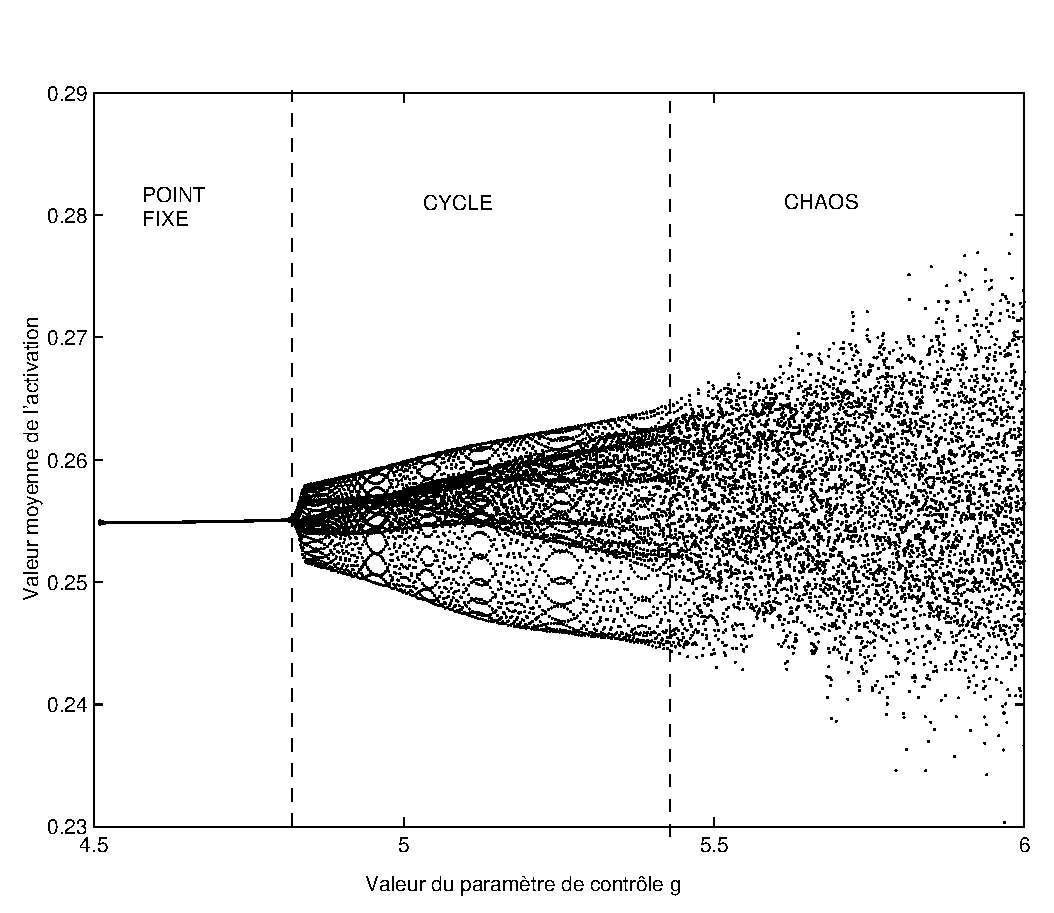
\includegraphics[width = 0.7\linewidth]{figs/hermes_diagr_bif.eps}
	}
	\caption{Transitions de phase.
		La figure représente l’activité moyenne d'un réseau récurrent aléatoire de 200 neurones sur 14 000 pas de temps,
		tandis que l’on augmente lentement le gain
		entre $g=4$ et $g=6$ (Beslon \& Daucé, 2002)}
	\label{fig:hermes-bif}
\end{figure} 


Il est intéressant de constater que le processus stochastique limite, tel que décrit par les équations de champ moyen, 
a une traduction à taille finie
sous la forme d'une activité de type \textit{chaos déterministe}. L'existence d'un 
paramètre de contrôle (le gain de la fonction de transfert des neurones) permet de reproduire, dans ces réseaux aléatoires, 
un  comportement générique de déstabilisation, appelé route vers le chaos par ``quasi-périodicité'' \shortcite{Berger1988,Doyon1993} (voir figure \ref{fig:hermes-bif}).
L'existence d'une telle frontière entre l'ordre et le chaos est également prouvée à la limite thermodynamique, mais dans ce
cas la transition se fait brutalement, avec un passage discret d'un processus de type point fixe à un processus stochastique \shortcite{Ces95}.
Cette frontière entre ordre et chaos est par principe intéressante puisqu'elle indique le lieu
où la variabilité de la dynamique, et donc potentiellement {\color{Orange} l'expressivité du réseau est la plus importante. }

\subsection{Réseaux équilibrés} \label{sec:balanced}

L'activité nerveuse est caractérisée par la présence fréquente d'oscillations collectives, souvent transitoires, 
observables à différentes échelles \shortcite{WangXJ2010}. 
%{\color{Orange} Le mécanisme par lequel une population de neurones peut se mettre à osciller 
%ont déjà été présentés dans la section \ref{sec:balanced}}. 

Les comportements oscillants ont été analysés de manière approfondie en modélisation à travers l'étude des réseaux de neurones dits ``équilibrés'' (\textit{balanced neural networks}).
Il s'agit d'une 
classe de réseaux de neurones constitués d'une population de neurones inhibiteurs et d'une population de neurones excitateurs.
Le terme ``équilibre'' se réfère ici à l'idée d'équilibre
dynamique entre deux forces opposantes~: la dynamique du réseau est amenée à converger vers un point d'équilibre
traduisant localement (et globalement) le ``poids'' des deux influences. 
\begin{itemize}
	\item Une configuration des poids se traduisant
	par une activité endogène soutenue 
	traduit une domination de l'influence excitatrice.
	\item A l'inverse, une configuration où l'activité intrinsèque disparaît après un certain temps 
	traduit une domination de l'influence inhibitrice.
\end{itemize} 

Comme dans le cas des réseaux aléatoires simples, il existe un paramètre de contrôle correspondant au rapport entre l'influence 
excitatrice et l'influence inhibitrice. 


De manière intéressante, une grande variété de comportements dynamiques peuvent être observés
à la frontière, et entre l'extinction et l'activité soutenue, comme les oscillations synchronisées \shortcite{brunel00} et/ou le chaos \shortcite{Van98}. 

\subsubsection{Rôle computationnel des oscillations synchronisées}
Plusieurs hypothèses ont été proposées sur le rôle
des oscillations synchronisées, 
\begin{itemize}
	\item comme mécanisme permettant de {\color{Orange} ``lier'' (assembler) les différentes modalités (constituants) d'un 
		même phénomène \shortcite{Gra89}}. La cohérence de phase
	observée à large échelle est vue comme la signature d'une activité coordonnée entre des aires séparées par plusieurs 
	centimètres \shortcite{Rod99}. 
	\item comme porteuse permettant une forme de cadençage et de séquençage des stimuli 
	dans les couches sensorielles primaires \shortcite{MLe96}. 
	\begin{itemize}
		\item Différents régimes oscillatoires sont classiquement identifiés, classifiés selon la
		bande de fréquence qu'ils occupent :  oscillations theta (3-8 Hz), oscillations alpha (10-15 Hz), oscillations beta (15-25 Hz) et
		oscillations gamma (> 30 Hz) \cite{Bremer1949}.
		\item L'anticipation de phase (phase précession) ou le retard de phase observés au niveau cellulaire dans 
		un contexte d'oscillations theta \shortcite{Skaggs1996}
		sont interprétés comme caractéristiques d'une activité au sein de laquelle l'ordre de tir 
		des potentiels d'action individuels joue un rôle important.
	\end{itemize}
\end{itemize} 

\subsection{Codage topographique et champ neuronal}\label{sec:NField}

Le modèle du ``champ neuronal'' est un modèle de type champ moyen, c'est à dire qu'il décrit les réseaux de neurones d'un point de vue macroscopique. L'activité de larges populations de neurones s'apparente en effet, à la limite des grandes tailles, à un milieu continu dans lequel chaque portion de l'espace peut être décrit par la ``densité'' d'activité qui s'y développe.

Le modèle le plus connu est décrit par des équation intégro-différentielles. Soit $x$ un point d'un espace (ou d'une portion d'espace) cartésien $\mathcal{X}$.
Dans le modèle d'Amari \shortcite{Ama77B}, les neurones sont décrits par leur potentiel d'activation $V$ et par la sortie binaire de la fonction d'activation $f$ (fonction de Heaviside).  Le potentiel d'activation d'un neurone est donné par l'équation~:
\begin{align}
\tau \frac{dV(x,t)}{dt} = -V(x,t) + I(x,t) - \theta + \int_{y \in \mathcal{X}} W(||x-y||) f(V(y,t)) dy
\end{align} 
où $I$ est un signal extérieur et $W$ un noyau décrivant les interactions réciproques entre neurones en fonction de la distance $||x - y||$.

Lorsque le noyau est 

\subsubsection{Rôle computationnel du codage topographique}

\subsection{Neurones impulsionnels}

\subsubsection{Rôle computationnel du codage impulsionnel}

%\subsection{Applications}

\cleardoublepage

\section{Contributions personnelles}

{\color{Cyan}
	Par rapport aux propositions, j'ai fait:
	\begin{itemize}
		\item ceci
		\item {\color{Orange} Proposition~: la présence d'une pulsation périodique permet d'implémenter les propriétés du neural field sans utiliser de mémoire cellulaire.}
		\item etc.
	\end{itemize}
}	

\subsection{Réseaux aléatoires multi-populations}\label{sec:multi_pop}
Une des premières études auxquelles j'ai participé portait sur les transitions de phase dans les réseaux de neurones
aléatoires. 
Les différentes architectures neuronales étudiées ont 
permis d'identifier des comportements caractéristiques, décrits sous la forme de différents régimes dynamiques. 
{\color{Orange} Nous avons cherché à caractériser l'expressivité de ces substrats, c'est à dire leur capacité à produire
des patrons d'activité pouvant servir de support à des opérations cognitives. }

\begin{figure}[b!]
	\centerline{
		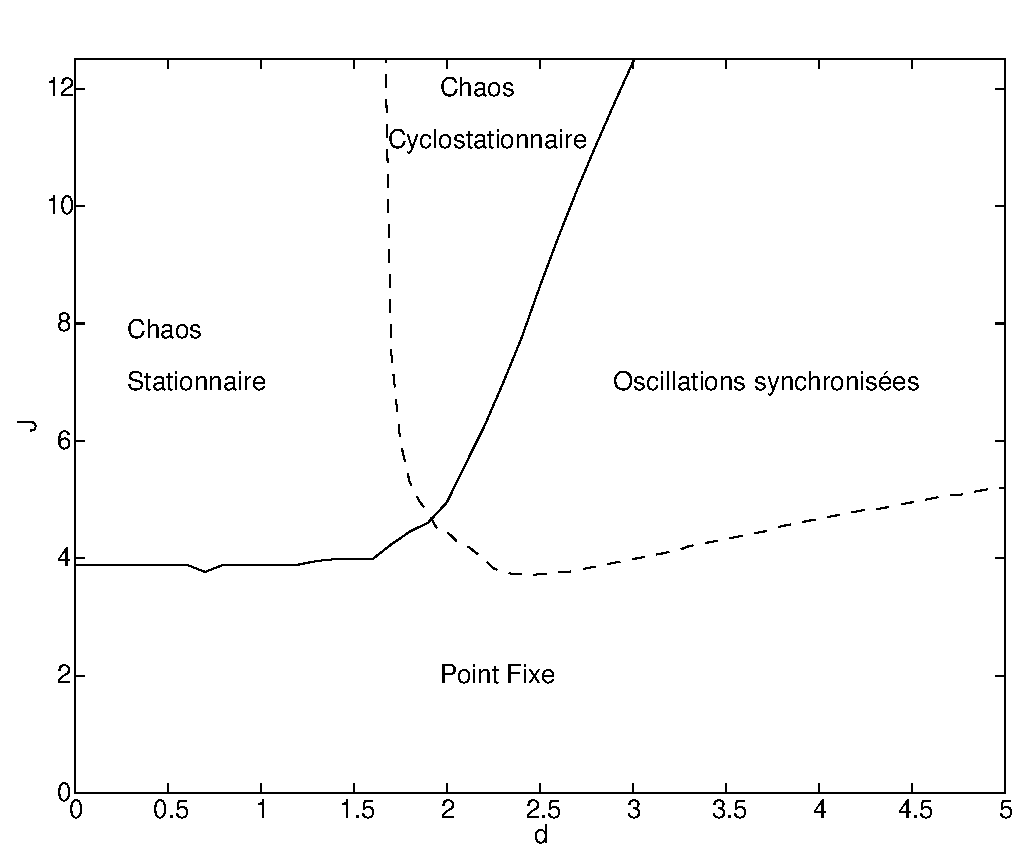
\includegraphics[width = 0.7\linewidth]{figs/map_2pop.eps}
	}
	\caption{Diagramme de bifurcation à la lite thermodynamique sur un réseau aléatoire équilibré à 2 populations, en fonction de $d$ (homogénéité) et $J$ (amplification).}
	\label{fig:diagr-2pop}
\end{figure} 

L'étude présentée dans \shortcite{Dau99A,dauce01a} étudie le comportement d'un réseau dit ``équilibré'' (voir section \ref{sec:balanced}). 
{\color{Gray} Le point de départ consistait à modéliser et reproduire certains comportements observés dans les 
réseaux de neurones naturels composés d'une population de neurones excitateurs et d'une population de neurones inhibiteurs (réseaux équilibrés,.}
Ce papier 
étend pour la première fois le modèle de champ moyen pour le cas des réseaux à connectivité aléatoire à populations multiples
(auquel cas les tirages aléatoires sont effectués sur des ``faisceaux d'axones'' reliant une population de neurones $p \in 1..K$ à une
population de neurones $q \in 1..K$, où $K$ est le nombre de populations).
Ce modèle renouvelle l'approche large-échelle classique \shortcite{WILSON89} en prenant en compte l'hétérogénéité des faisceaux
d'axones reliant différentes régions du réseau.  
Il sert de base à la définition d'architectures neuronales fondées sur des 
substrats à connectivité aléatoire. 

%{\color{Violet}
%[Multi-pop = base pour l'approche multi-échelle. Construction / architecture neuronale. Prise en compte de l'hétérogénéité.]
%Multi-pop = travail de master d'O Pinaud.
%Demonstration champ moyen = O Moynot (avec généralisation à la connectivité diluée)}

L'étude numérique proposée dans le papier fixe le rapport excitation/inhibition à $\frac{1}{2}$,
ce qui correspond à un régime de faible activité \shortcite{Amit1989}. 
Nous étudions le rôle contrasté de deux paramètres de contrôle (voir Figure \ref{fig:diagr-2pop}). 
\begin{itemize}
	\item Le premier paramètre, $J$, représente l'amplification du signal. L'augmentation
	continue de ce paramètre tend à produire une bifurcation entre un régime simple (point fixe) et une activité 
	complexe (de type chaotique) {\color{Orange} comme précédemment.}
	\item Un second paramètre, nommé $d$, représente l'inverse du \textit{coefficient de variation} des liens, autrement dit le 
	degré d'homogénéite. Augmenter ce paramètre tend à rendre les poids plus homogènes. 
\end{itemize}
De manière intéressante, 
l'augmentation continue de ce second paramètre (augmentation de l'``ordre'') produit une transition 
entre un régime stationnaire et un régime non-stationnaire périodique. Nous mettons en évidence une carte
de bifurcation à 4 régions, comprenant un régime stationnaire de point fixe, un régime stationnaire complexe,
un régime d'oscillations simple, et un régime d'oscillations complexes analogue à processus stochastique cyclostationnaire,
ce dernier régime étant à notre connaissance mis en évidence pour la première fois dans ce type de réseaux.





Notre étude a donc ouvert la voie à l'étude multi-population systématique des réseaux de neurones à connectivité aléatoire,
voir par exemple \shortcite{Faugeras2009,Cabana2013}. %L'accent sur l'équilibre dynamique entre populations escitatrice et inhibitrice

{\color{Orange}[CITER SOULA-BESLON] et ECM avec IF neurons}


%{\color{Violet}
%[O. Faugeras, J. Touboul, B. Cessac, “A constructive mean field analysis of multi population neural networks with random synaptic weights and stochastic inputs”, Front. Comput. Neurosci. (2009) 3:1.

%et aussi 

%Large Deviations, Dynamics and Phase Transitions in Large Stochastic and Disordered Neural Networks
%Tanguy Cabana1 and Jonathan Touboul (2013)

%La question de l'homogénéité/hétérogénéité est revenue à l'ordre du jour. Plusieurs papiers récents bla bla...}

%\cleardoublepage
%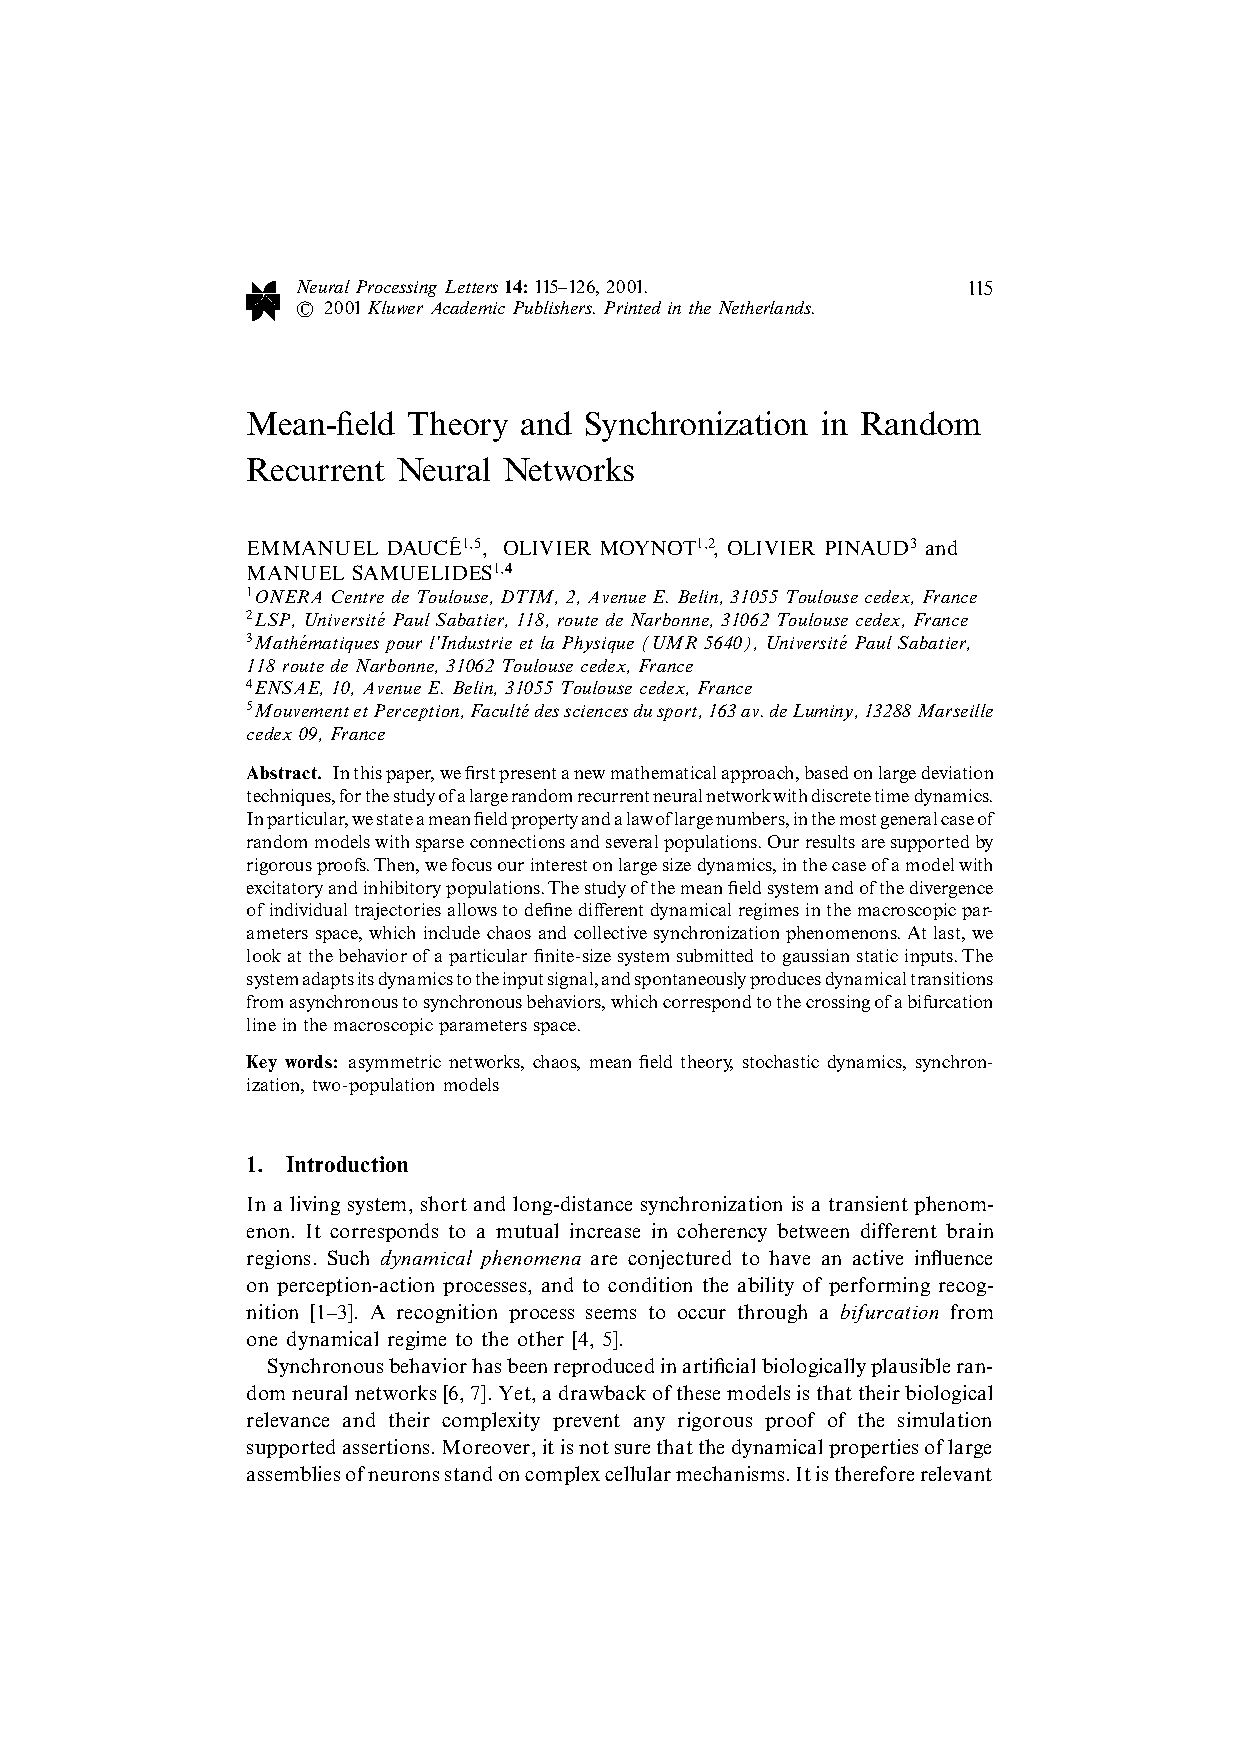
\includepdf[pages=1-2,landscape=true,nup=1x2,scale=1.1,offset= 70 -30]{pdf/2001-neural-proc-letters.pdf}
%\includepdf[pages=3-4,landscape=true,nup=1x2,scale=1.1,offset= -70 -30]{pdf/2001-neural-proc-letters.pdf}
%\includepdf[pages=5-6,landscape=true,nup=1x2,scale=1.1,offset= 70 -30]{pdf/2001-neural-proc-letters.pdf}
%\includepdf[pages=7-8,landscape=true,nup=1x2,scale=1.1,offset= -70 -30]{pdf/2001-neural-proc-letters.pdf}
%\includepdf[pages=9-10,landscape=true,nup=1x2,scale=1.1,offset= 70 -30]{pdf/2001-neural-proc-letters.pdf}
%\includepdf[pages=11-12,landscape=true,nup=1x2,scale=1.1,offset= -70 -30]{pdf/2001-neural-proc-letters.pdf}

\cleardoublepage
\subsection{Criticalité dans les réseaux aléatoires}

Un des intérêts principaux des réseaux à connectivité aléatoire est leur capacité à générer des dynamiques complexes
endogènes (donc sans stimulation extérieure). Ces dynamiques, bien que reposant sur des équations déterministes,
se comportent comme des processus stochastique indépendants sur chaque neurone. Ce comportement n'est pourtant pas analogue
à un simple bruit passif. 

\begin{figure}[b!]
	\centerline{
		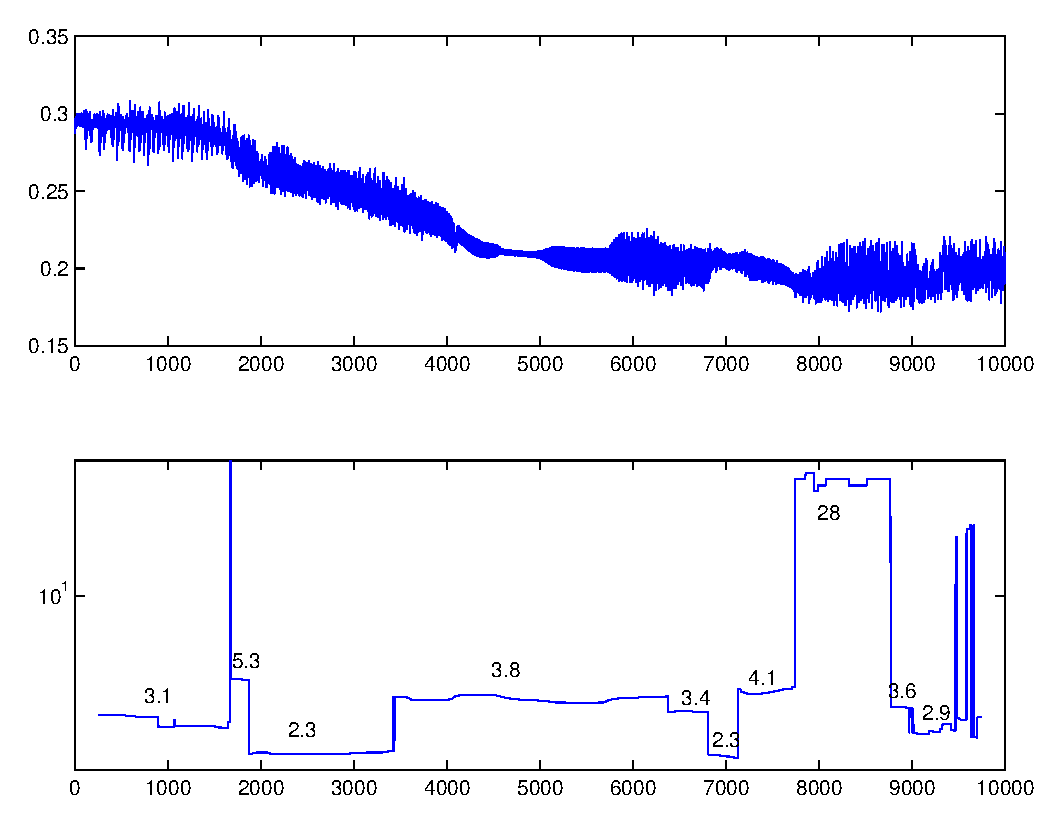
\includegraphics[width = 0.7\linewidth]{figs/simu_derive_periodes_x2.eps}
	}
	\caption{Activité d'un réseau récurrent aléatoire de 200 neurones, sur 10000 pas de temps, sous l’influence d'une entrée sensorielle à évolution lente. La période principale est estimée par spectre de Fourier sur
		une fenêtre de 500 pas de temps (cette période étant représentative de la période propre de
		chaque neurone actif). a) Activité moyenne. b) 
		Période du mode principal (en échelle logarithmique) (Beslon \& Daucé, 2002)}
	\label{fig:hermes-critic}
\end{figure} 


Une manière simple de caractériser le comportement non-linéaire (ou critique) d'une population de neurones consiste à introduire de petites perturbations
dans la dynamique du réseau. 
Une étude proposée dans le 3ème chapitre de l'ouvrage que nous avons co-dirigé avec Agnès Guillot \shortcite{Beslon2002} illustre le propos.
Cette étude porte sur le modèle le plus simple, un réseau récurrent aléatoire comportant une seule population. Le paramètre de contrôle
choisi place le réseau dans une région chaotique, proche de la transition vers le cycle limite.  
Le réseau est soumis à une stimulation extérieure quasi stationnaire, évoluant à une vitesse très lente par rapport à la vitesse de 
mise à jour du réseau. Une succession de régimes dynamiques distincts, séparés par des transitions brusques, est mise en évidence (voir figure \ref{fig:hermes-critic}).
Chaque régime est caractérisé par un patron d'activité différent, qui se manifeste par la présence de fréquences caractéristiques
distinctes dans le spectre de Fourier du signal moyen. 

% DONNEES A REPRENDRE SUR SIMU99_0726.mat
\begin{figure}[b!]
	\centerline{
		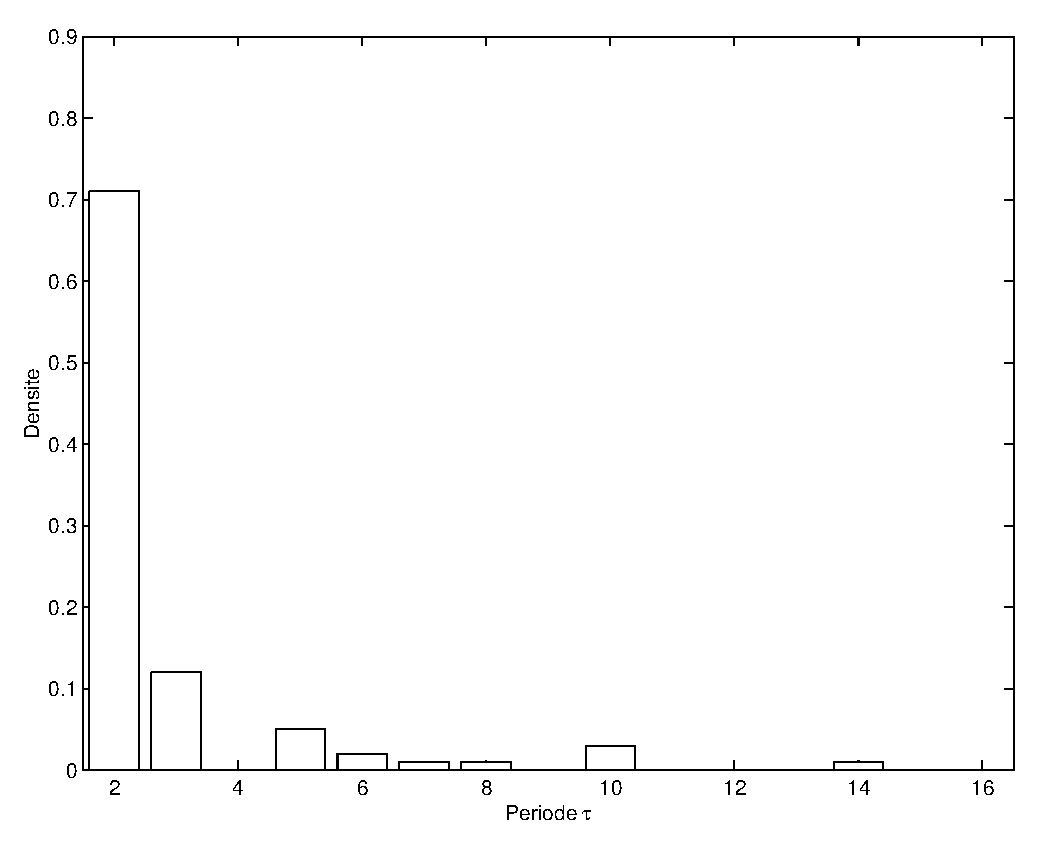
\includegraphics[width=0.3\linewidth]{figs/hist_periode_2.eps}
		\hspace{0.5cm}
		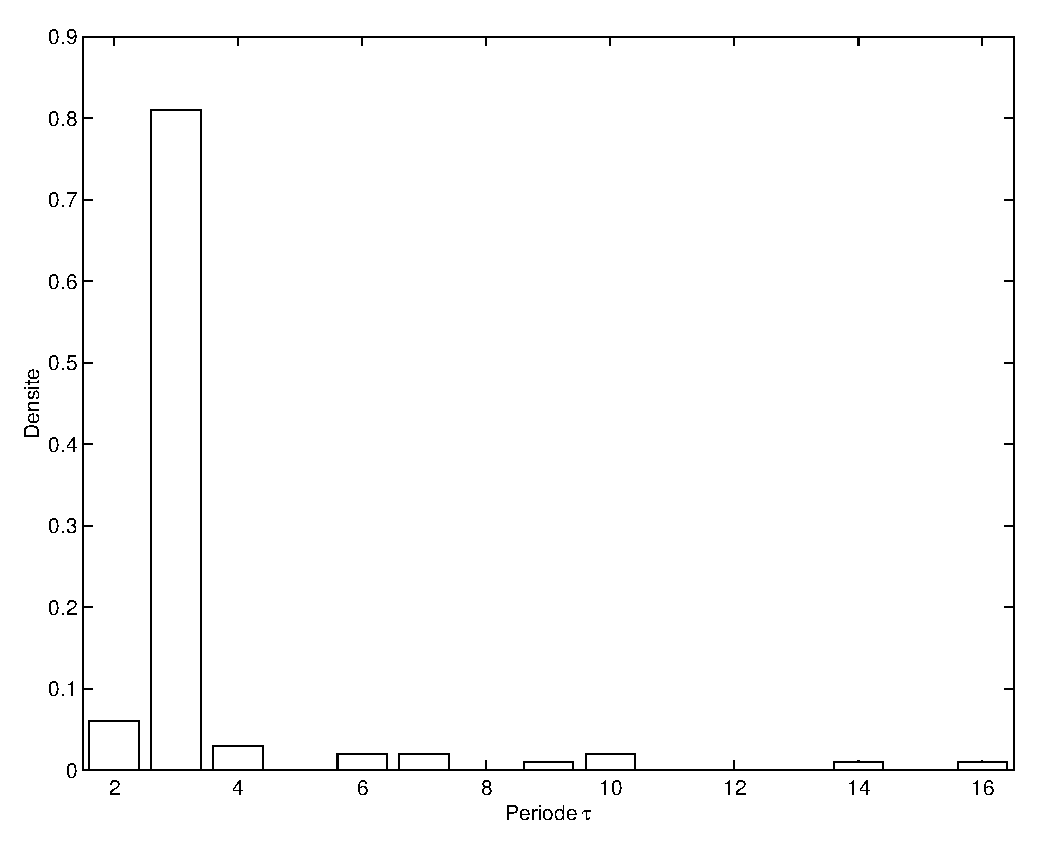
\includegraphics[width=0.3\linewidth]{figs/hist_periode_3.eps}
		\hspace{0.5cm}
		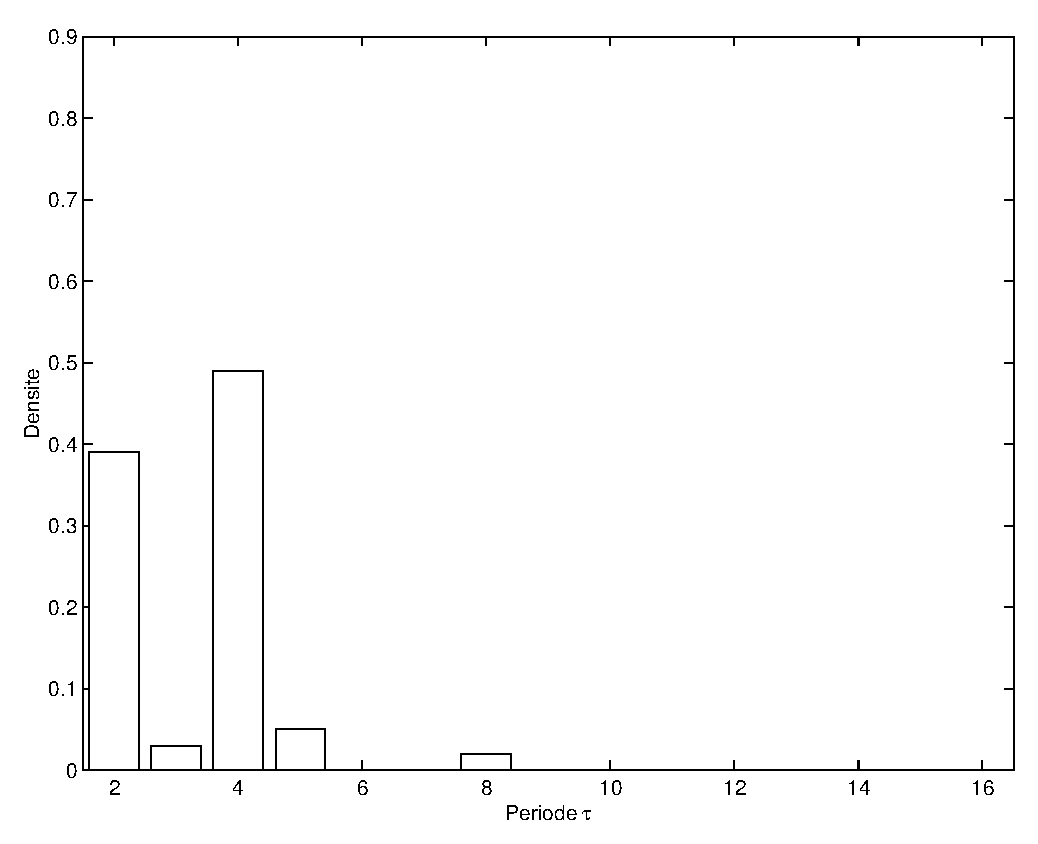
\includegraphics[width=0.3\linewidth]{figs/hist_periode_4.eps}
	}
	\centerline{
		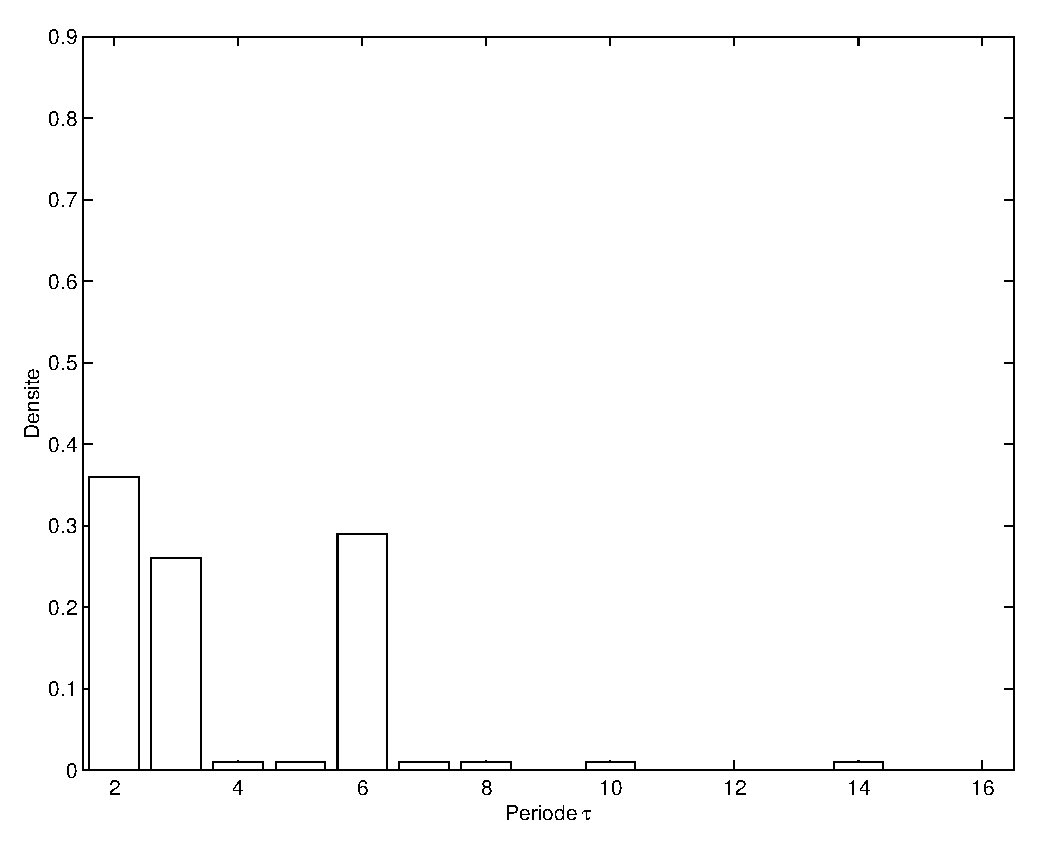
\includegraphics[width=0.3\linewidth]{figs/hist_periode_6.eps}
		\hspace{0.5cm}
		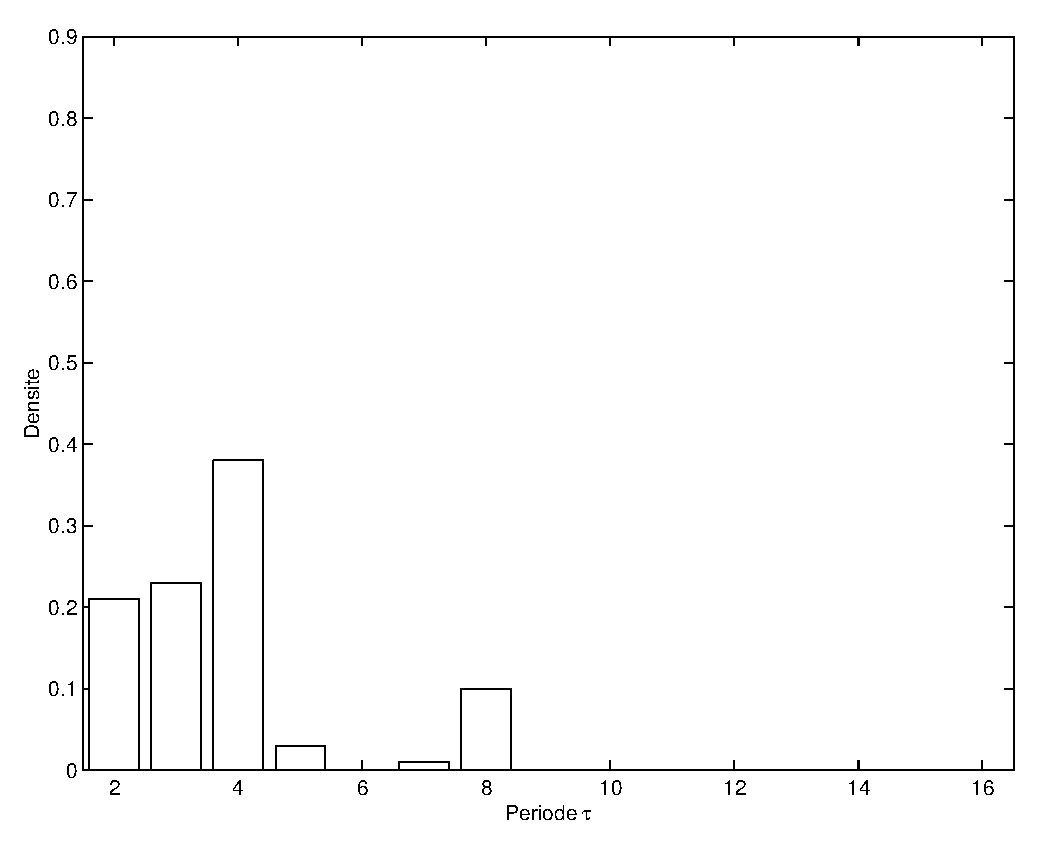
\includegraphics[width=0.3\linewidth]{figs/hist_periode_8.eps}
		\hspace{0.5cm}
		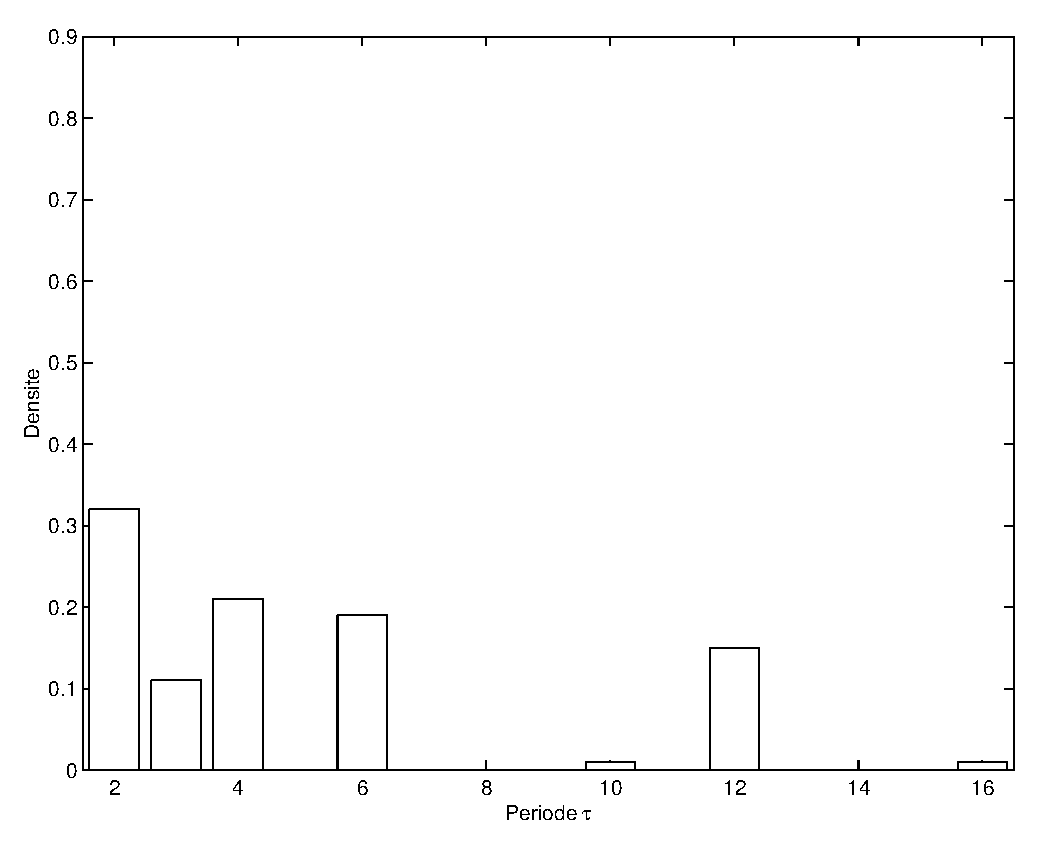
\includegraphics[width=0.3\linewidth]{figs/hist_periode_12.eps}
	}
	\caption{{\bf Capture de p\'eriode pour diff\'erentes valeurs de $\tau$ (période du signal).}
		On a repr\'esent\'e sur ces histogrammes la r\'epartition des p\'eriodes, mesur\'ee sur 100 couples (r\'eseau, s\'equence d'entrée) pour $\tau=2$ (haut, gauche), $\tau=3$ (haut, milieu), $\tau=4$ (haut, droite), $\tau=6$ (bas, gauche), $\tau=8$ (bas, milieu) et $\tau=12$ (bas, droite).
		Param\`etres~: $N=200$, $g=8$, $\bar{I}=0$, $\mu_{\theta}=0$, $\sigma_\theta=0$, $\mu_{J}=0$, $\sigma_J=1$, $\sigma_I=0.1$ (Daucé, 2001).
	}
	\label{fig:periode_expl}
\end{figure}


Une autre étude, présente dans mon manuscrit de thèse \shortcite{Dau00}, développe l'analyse spatio-temporelle des patrons d'activité de type cycle limite
ou chaos léger.
L'existence d'une chaîne d'activation spontanée (synfire chain \shortcite{ABELES91}) est mise en évidence par analyse de la matrice de covariance des signaux individuels. 
Différents modes (patrons d'activation spatio-temporels) se développent spontanément lorsque le réseau est soumis à des entrées statiques différentes \shortcite{Dau00b}.
Enfin, l'analyse de la réponse du réseau à une stimulation périodique indique une ``bande passante'' de quelques unités temporelles, le réseau étant capable 
de ``capturer'' (et donc d'amplifier) des signaux dont la période varie entre 2 et 10\--12 unités de temps
(autrement dit à sélectionner un mode dynamique périodique interne compatible avec la période imposée) \shortcite{Dau00b} \--- voir figure \ref{fig:periode_expl}.
Le comportements spontané des réseaux récurrents aléatoires est par ailleurs à la base du mécanisme de perception par feedback positif
présentés dans la section \ref{sec:BioCyb02}. 

L'intérêt du comportement spontané des réseaux récurrents à connectivité aléatoires a été largement confirmé depuis. 
Une étude plus systématique de la réponse linéaire dans les réseaux récurrents \shortcite{Cessac2007} met en évidence 
l'existence de modes et de résonances extrêmement variés lorsque le signal est applique sur un seul noeud du réseau (micro-stimulation). 
Les modèles de ``réservoir
computing'' proposés par l'équipe de Wolfgang Maas \shortcite{Maass2002} reposent sur le même principe : un réseau de neurones aléatoire récurrent soumis à un signal
spatio-temporel est capable de conserver une mémoire de quelques unités de temps utilisables pour produire des classifieurs sensibles
au contexte temporel.

{\color{Cyan} Image du papillon-chenille.}

Ce modèle de réseau à connexions aléatoire offre un exemple de substrat dont la caractéristique principale est la \textit{capture dynamique}, reposant
sur des transformations morphologiques des patrons d'activités (changements des distributions spatiales et temporelles des activités). Bien que construits sur
un tirage aléatoire arbitraire, ils offrent donc un bon support pour le traitement (et la transformation) des signaux temporels. 
Faire reposer le traitement sur un tirage arbitraire rejoint d'ailleurs un certain nombre de techniques de plongement (ou projection) aléatoires
utilisées en apprentissage automatique, tels le ``compressive sensing'' \shortcite{Baraniuk2007} ou l'architecture ``extreme learning'' \shortcite{Huang2006}.

%\cleardoublepage
%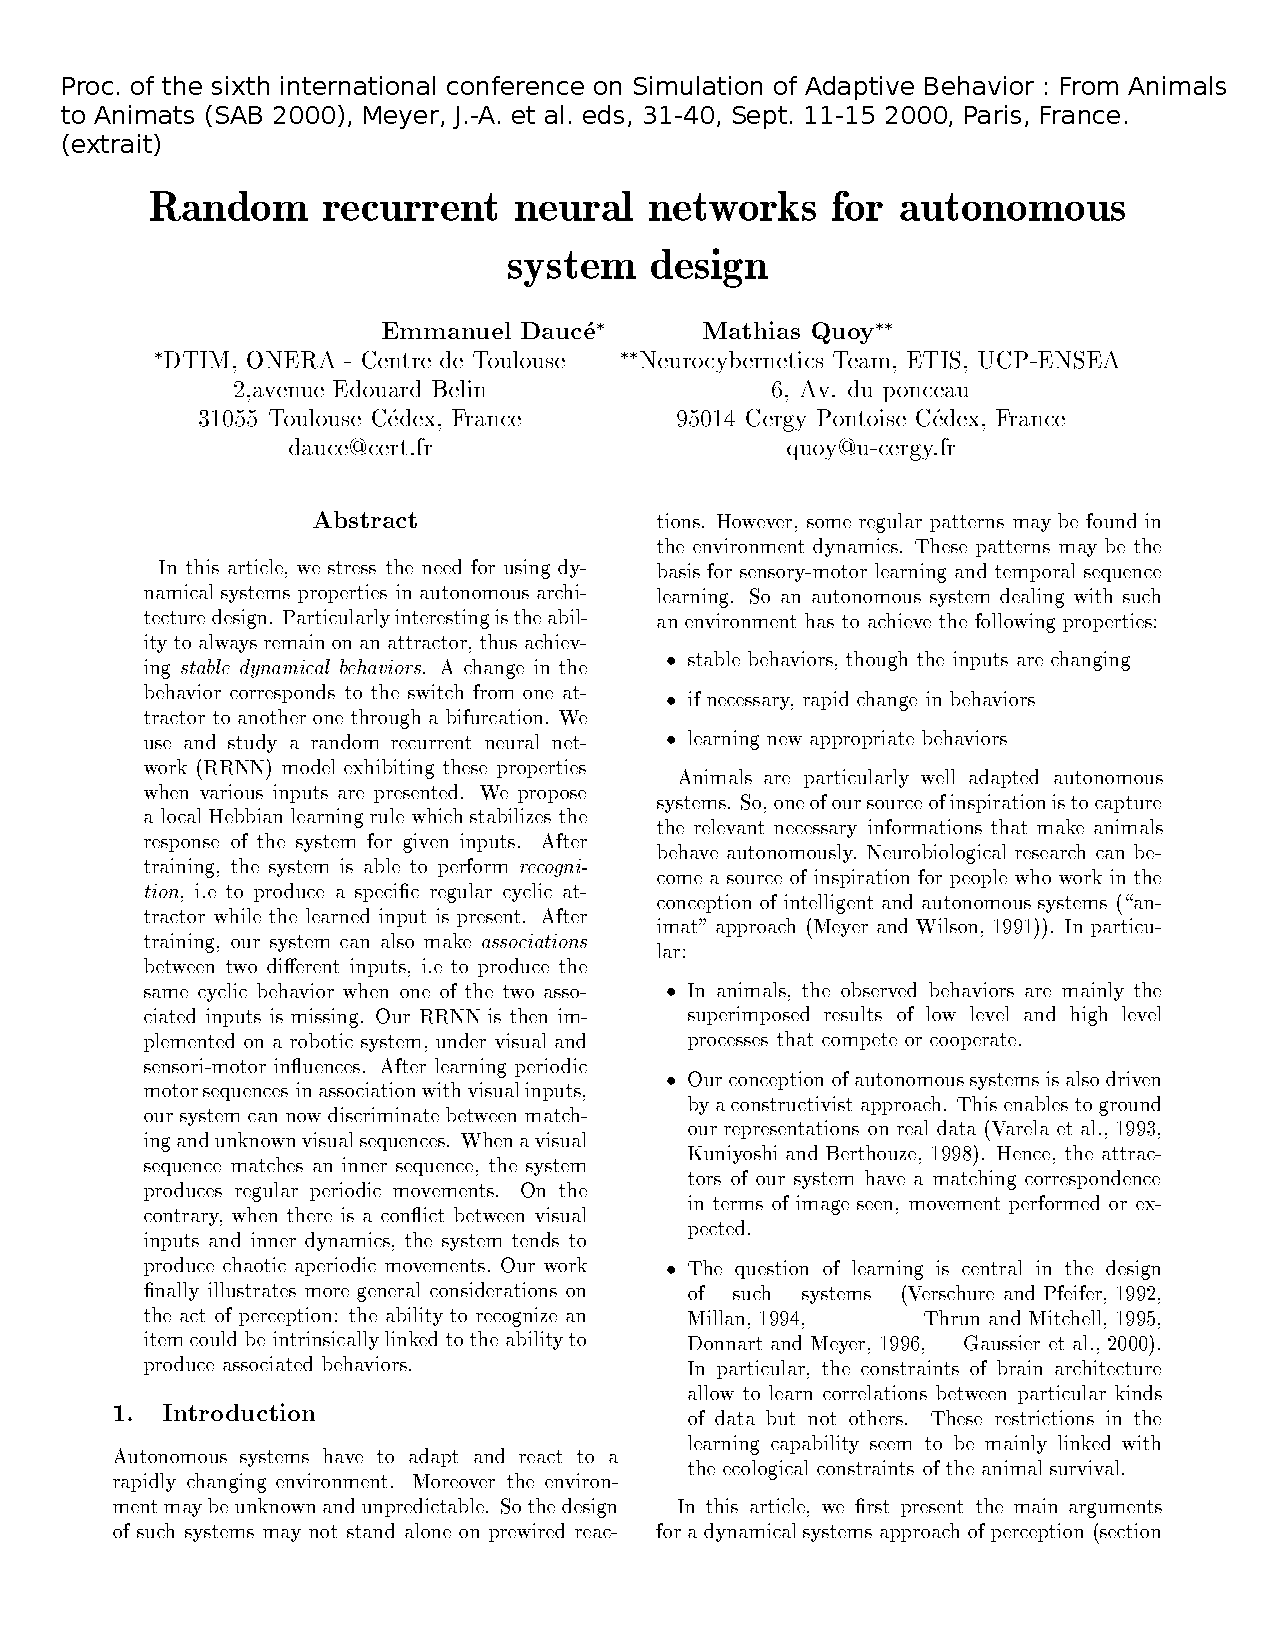
\includepdf[pages=1, offset=70 -20]{pdf/2000-sab-ann.pdf}
%\includepdf[pages=2, offset=-70 -20]{pdf/2000-sab-ann.pdf}
%\includepdf[pages=3, offset=70 -20]{pdf/2000-sab-ann.pdf}
%\includepdf[pages=4, offset=-70 -20]{pdf/2000-sab-ann.pdf}
%\includepdf[pages=18, offset=70 -50]{pdf/2007-epj-st-ann2.pdf}
%\includepdf[pages=19, offset=-70 -50]{pdf/2007-epj-st-ann2.pdf}
%\includepdf[pages=20, offset=70 -50]{pdf/2007-epj-st-ann2.pdf}
%\includepdf[pages=21, offset=-70 -50]{pdf/2007-epj-st-ann2.pdf}
%\includepdf[pages=22, offset=70 -50]{pdf/2007-epj-st-ann2.pdf}
%\includepdf[pages=23, offset=-70 -50]{pdf/2007-epj-st-ann2.pdf}
%%%%%%%%%%%%%%%%%%%%%%%%%%%%%%%%%%%%%%%%%%%%%%%%%%%%%%%%%%%%%%%%%%%%%%%%%%%%%%%%%%%%%%%%%%%%%%%%%%%%%%%%%%%%%%%%%%%
%%%%%%%%%%%%%%%%%%%%%%%%%%%%%%%%%%%%%%%%%     1.3      %%%%%%%%%%%%%%%%%%%%%%%%%%%%%%%%%%%%%%%%%%%%%%%%%%%%%%%%%%%%
%%%%%%%%%%%%%%%%%%%%%%%%%%%%%%%%%%%%%%%%%%%%%%%%%%%%%%%%%%%%%%%%%%%%%%%%%%%%%%%%%%%%%%%%%%%%%%%%%%%%%%%%%%%%%%%%%%%

%%%%%%%%%%%%%%%%%%%%%%%%%%%%%%%%%%%%%%%%%%%%%%%%%%%%%%%%%%%%%%%%%%%%%%%%%%%%%%%%%%%%%%%%%%%%%%%%%%%%%%%%%%%%%%%%%%%
%%%%%%%%%%%%%%%%%%%%%%%%%%%%%%%%%%%%%%%%%     1.2      %%%%%%%%%%%%%%%%%%%%%%%%%%%%%%%%%%%%%%%%%%%%%%%%%%%%%%%%%%%%
%%%%%%%%%%%%%%%%%%%%%%%%%%%%%%%%%%%%%%%%%%%%%%%%%%%%%%%%%%%%%%%%%%%%%%%%%%%%%%%%%%%%%%%%%%%%%%%%%%%%%%%%%%%%%%%%%%%

\cleardoublepage
\subsection{Modèles de champ neuronal}\label{sec:NatComp}

La question adressée par le modèle publié en 2004 \shortcite{Dau04} est celle de l'implémentation d'un modèle de champ neuronal (voir section \ref{sec:NField}) sur un support composé
d'unités discrètes.
%, comme l'activité dite ``persistante'' ainsi qu'une bonne sensibilité au signal d'entrée (switch). 
Sur les modèles jusqu'alors proposés, dans un cas l'activité focale était soit uniquement réactive \shortcite{Han96},  
dans l'autre cas,
l'activité persistante reposait sur un mécanisme de bistabilité cellulaire \shortcite{Cam98} ou encore sur une
plasticité synaptique à court terme \shortcite{Com00}. 
Notre modèle est une des premières implémentations d'un champ neuronal sur support discret reposant sur des mécanismes de réseau
uniquement.

Le papier étend le modèle récurrent aléatoire \shortcite{Dau01a} à des connectivités
plus complexes, incluant des délais variables et les connexions dépendantes de la distance. 
Un des apports du papier est de montrer 
la stabilité de certains indicateurs (comme le niveau de réponse moyen) à travers les modèles. 
Par exemple, l'introduction de délais différents entre les populations excitatrices et les populations inhibitrices conduit 
à des changements qualitatifs (régime d'oscillations lentes synchronisées) mais non quantitatif (même réponse
moyenne). 

L'introduction d'une connectivité dépendante de la distance opère un changement plus radical, 
puisque l'hypothèse fondatrice du modèle (indépendance des tirages) n'est plus vérifiée, 
et donc l'hypothèse de chaos local (indépendance des activités) n'est plus valide.
Les unités neuronales de chaque population reçoivent des coordonnées spatiales (ici prises uniformément sur un intervalle borné). %$[-\pi,\pi]$).
Le tirage des poids synaptiques devient dépendant de la distance qui sépare deux unités.
La valeur moyenne d'un poids est identique à celle du modèle précédent, 
mais les noeuds les plus proches ont en espérance une valeur
plus forte, et les noeuds les plus éloignés une valeur plus faible 
(la distribution des poids synaptiques repose sur le produit
entre la distribution uniforme initiale et un noyau gaussien conservatif).
Le mécanisme du champ neuronal, qui se caractérise par une connectivité majoritairement excitatrice à 
courte distance, et inhibitrice à longue distance, est implémenté à l'aide de ces noyaux gaussiens 
tels que le rayon du noyau des liens excitateurs est plus faible que celui des liens inhibiteurs.  

Le papier montre alors que les propriétés des réseaux aléatoires récurrents et celles des champs neuronaux s'additionnent dans ce modèle,
puisqu'on peut mettre en évidence sur ce substrat la présence simultanée d'une activité de fond chaotique,
de grandes oscillations lentes et de foyers d'activité de type champ neuronal. 
Comme dans le cas du champ neuronal, l'activité persistante repose sur l'activité excitatrice locale, avec 
un effet de lissage lié à l'hétérogénéité des connexions. Les oscillations lentes reposent comme précédemment
l'existence de délais différenciés. Ce sont ces oscillations qui donnent au substrat 
la capacité de répondre à des changements de faible amplitude (augmentent donc la sensibilité 
du substrat au signal d'entrée). Il en résulte une implémentation d'un champ neuronal 
sur un substrat composé d'unités neuronales discrètes.

De manière plus générale, ce modèle nous fournit un premier exemple, dans le cadre des réseaux récurrents aléatoires,
de l'effet de mémoire produit par une boucle de rétroaction positive. 

Notre modèle propose une passerelle simple entre les modèles de champ neuronal continus et de
réseaux de neurones à état et à temps discret. 
Il s'étend facilement à des réseaux de neurones intègre-et-tire (non publié), avec des
%L'activité produite repose néanmoins essentiellement sur la fréquence de tir des neurones (et non sur l'ordre de tir
%ou la co-activation). Les propriétés obtenues ne sont donc 
propriétés peu différentes qualitativement de celles qu'on 
obtient avec des modèles à fréquence de décharge.
Ce modèle a été utilisé en tant que couche perceptive dans des architectures de contrôle \shortcite{Dau04b,Dau07}. 
D'autres modèles visant une plus grande fidélité aux processus biologiques 
ont étudié l'effet de délais variables et de patrons de connexion hétérogènes (voir par exemple \shortcite{Roxin2005}),
et plus généralement l'étude de l'interaction entre délais variables, topographie et dynamique reste un sujet d'actualité 
en neurosciences computationnelles \shortcite{Voges2012,Lundqvist2012}.

\cleardoublepage
\subsection{Modèles de la connectivité fonctionnelle large-échelle}

L'apparition récente des techniques de tractographie par tenseurs de diffusion \shortcite{leBihan2001} permet d'analyser 
la matière blanche du cerveau pour suivre la direction des  faisceaux de fibres. 
Il est possible d'en déduire un patron de connectivité (le ``connectome'') reliant les principales régions du cortex. 
Le patron de connectivité issu de cette analyse forme un réseau, constitué par deux matrices, l'une fournissant la distance entre les
régions connectées, l'autre fournissant le ``poids'' de cette connexion en fonction de la densité de fibres.
Ce réseau est relativement stable à travers les sujets.
%Différents indicateurs globaux ont été proposés [CIITATIONS] dont la déviation par rapport 
%à la moyenne vise à repérer (ou améliorer l'identifications) de pathologies [CITATIONS].

Le connectome offre une vue d'ensemble de l'architecture du cerveau.
L'analyse du connectome (analyse ``structurelle'')  vient en complément
de l'analyse des patrons d'activité observés dans l'exercice d'une tâche (analyse fonctionnelle).
%(les mêmes grandes autoroutes sont présentes)
Dans le cadre de cette analyse structurelle, 
plusieurs indicateurs ont été proposées pour distinguer les noeuds les plus centraux (les plus ``importants'')
des noeuds périphériques. Il est possible de mettre en évidence d'un ``noyau central'' \shortcite{Hagmann2008}  
regroupant des noeuds médians servant de lien (ou de relais) entre la plupart des autres régions.
Cet ensemble de noeuds présente des points communs avec le patron d'activité ``par défaut'' observé en imagerie fonctionnelle 
(l'activité observée lorsque le sujet n'est pas occupé à accomplir une tâche) \shortcite{Raichle2001}. 

En partant de la structure du connectome, nous avons utilisé pour l'activation des noeuds
différentes variantes du modèle ``à réponse graduelle'' de Hopfield \shortcite{Hopfield1984}, 
en changeant les caractéristiques du seuil d'activation afin de contrôle le niveau d'activation moyen.
Ces travaux ont permis de mettre en évidence un nombre très important d'attracteurs dans certaines gammes de paramètres.
Ainsi, en condition de ``basse température'', le nombre d'attracteurs distincts peut atteindre plusieurs milliers
(sur un modèle comportant 998 noeuds). %cette prolifération d'attracteurs est un indicateur du caractère 
L'analyse des ensembles d'attracteurs obtenus permet d'identifier une douzaine de ``modes'' différents, chaque
mode correspondant à l'activation d'une région anatomique particulière. Ces modes peuvent être comparés aux modules 
régionaux mis en évidence par une analyse structurelle \shortcite{Hagmann2008} ainsi qu'avec les composants indépendants 
identifiés sur les signaux fMRI de l'état de repos \shortcite{Damoiseaux2006}.

L'ajout d'un terme de bruit dans l'équation de mise à jour permet de simuler une activité multistable \emph{temporellement}, 
s'apparentant aux régimes dits de ``dynamique itinérante'' \shortcite{Tsuda92,Kan90},
et dont les caractéristiques sont plus proches des signaux observés à l'état de repos. 
Cette multistabilité temporelle conduit fréquemment le réseau vers des régimes d'activité plus simples 
(noeuds uniformément actifs
ou inactifs) par dérive lente de l'activité moyenne. 
Seul un modèle à ``feedback négatif global'' présente une multistabilité temporelle à long terme,
grâce au contrôle du niveau d'activité  qui empêche d'atteindre les régimes triviaux.

%{\color{Violet}

%{\bf 2011}

%- approche Hopfield / connectome. Adatron pour “connectome inverse”

%{\bf 2012}

%- Connectome-based simulation : multistabilité spatiale et temporelle 

%{\bf 2014}

%- Connectome : identification de patchs à travers les patrons statiques (modele verre de spin). 

%RSN

%DTI

%dualité covariance/causalité. 

%connectivité structurelle / fonctionnelle
%}

%\cleardoublepage
%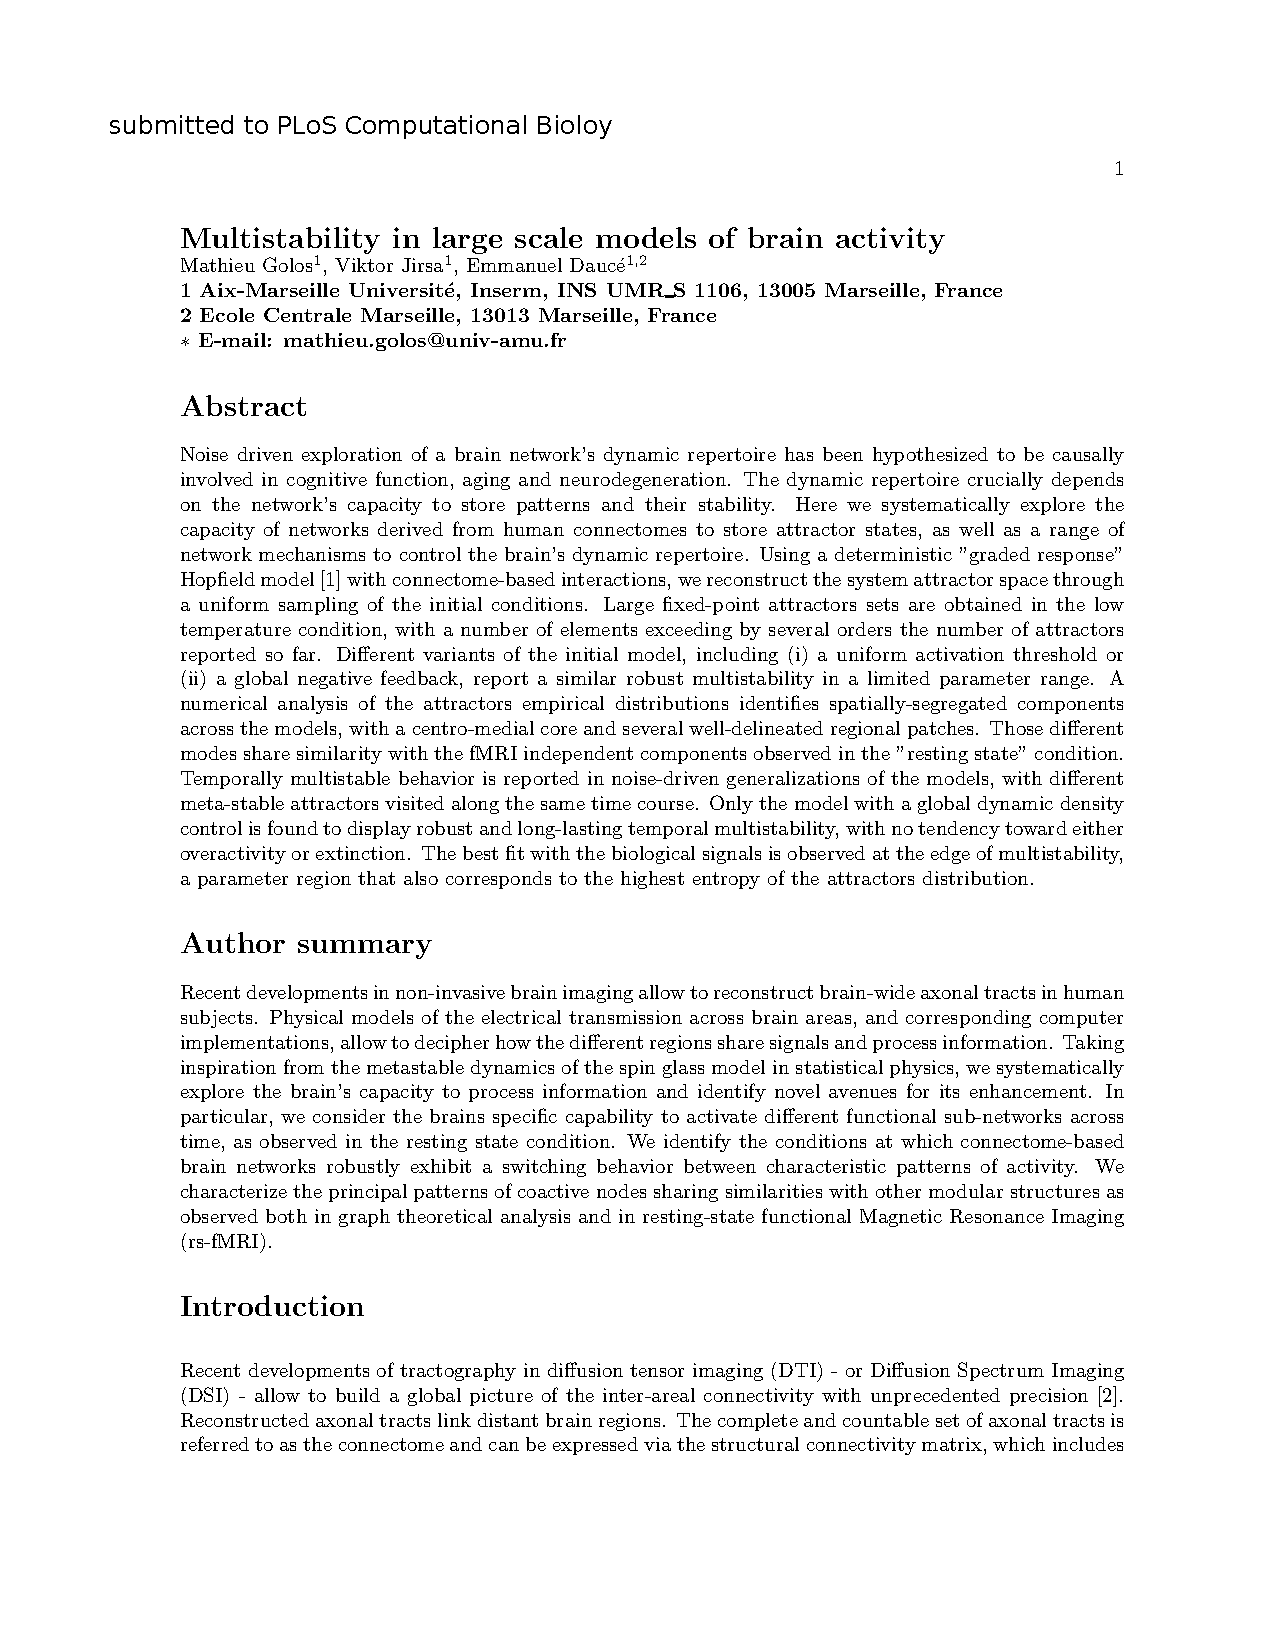
\includepdf[pages=1,offset=70 -20]{pdf/2015-PLOS-CB-ann.pdf}
%\includepdf[pages=2,offset=-70 -20]{pdf/2015-PLOS-CB-ann.pdf}
%\includepdf[pages=3,offset=70 -20]{pdf/2015-PLOS-CB-ann.pdf}
%\includepdf[pages=4,offset=-70 -20]{pdf/2015-PLOS-CB-ann.pdf}
%\includepdf[pages=5,offset=70 -20]{pdf/2015-PLOS-CB-ann.pdf}
%\includepdf[pages=6,offset=-70 -20]{pdf/2015-PLOS-CB-ann.pdf}
%\includepdf[pages=7,offset=70 -20]{pdf/2015-PLOS-CB-ann.pdf}
%\includepdf[pages=8,offset=-70 -20]{pdf/2015-PLOS-CB-ann.pdf}
%\includepdf[pages=9,offset=70 -20]{pdf/2015-PLOS-CB-ann.pdf}
%\includepdf[pages=10,offset=-70 -20]{pdf/2015-PLOS-CB-ann.pdf}
%\includepdf[pages=11,offset=70 -20]{pdf/2015-PLOS-CB-ann.pdf}
%\includepdf[pages=12,offset=-70 -20]{pdf/2015-PLOS-CB-ann.pdf}
%\includepdf[pages=13,offset=70 -20]{pdf/2015-PLOS-CB-ann.pdf}
%\includepdf[pages=14,offset=-70 -20]{pdf/2015-PLOS-CB-ann.pdf}
%\includepdf[pages=15,offset=70 -20]{pdf/2015-PLOS-CB-ann.pdf}
%\includepdf[pages=16,offset=-70 -20]{pdf/2015-PLOS-CB-ann.pdf}
%\includepdf[pages=17,offset=70 -20]{pdf/2015-PLOS-CB-ann.pdf}
%\includepdf[pages=18,offset=-70 -20]{pdf/2015-PLOS-CB-ann.pdf}
%\includepdf[pages=19,offset=70 -20]{pdf/2015-PLOS-CB-ann.pdf}
%\includepdf[pages=20,offset=-70 -20]{pdf/2015-PLOS-CB-ann.pdf}
%\includepdf[pages=21,offset=70 -20]{pdf/2015-PLOS-CB-ann.pdf}
%\includepdf[pages=22,offset=-70 -20]{pdf/2015-PLOS-CB-ann.pdf}
%\includepdf[pages=23,offset=70 -20]{pdf/2015-PLOS-CB-ann.pdf}
%\includepdf[pages=24,offset=-70 -20]{pdf/2015-PLOS-CB-ann.pdf}



\chapter{Plasticité synaptique et apprentissage}
Ce chapitre est consacré à l'étude des mécanismes d'apprentissage dans les réseaux de neurones récurrents.  

{\color{Cyan} Il est organisé en trois sections:
\begin{itemize}
	\item bla bla
	\item bla bla	
	\item bla bla
\end{itemize}
}

\section{Notions générales}

\cleardoublepage

\subsection{Plasticité synaptique}

La synapse biologique est l'interface permettant la communication entre les neurones.
Il s'agit d'une petite surface d'échange chimique (``bouton'' synaptiques) située à l'extrémité de l'arborisation terminale des axones. A l'arrivée d'un potentiel d'action, les synapses libèrent des neurotransmetteurs qui agissent sur les canaux ioniques des dendrites de la cellule post-synaptique (``libèrent'' des ions), ce qui a pour effet de modifier le potentiel de membrane de la cellule post-synaptique.

L'efficacité d'une synapse dépend de plusieurs facteurs, comme la taille du bouton synaptique, la quantité de neurotransmetteurs disponibles,  ainsi que la sensibilité de la cellule post-synaptique. Dans le cadre de ce mémoire,  cet ensemble de facteurs est résumé  sous la forme d'une valeur unique $J_{ij}$ : le ``poids'' de la synapse, où  $j$ est l'index du neurone pré-synaptique et $i$ l'index du neurone post-synaptique.

La plasticité synaptique est un mécanisme biologique qui modifie l'efficacité de la synapse au cours du temps. En reprenant 
les notations de l'équation (\ref{eq:SD}), 
\begin{align}
&\boldsymbol{x}' = \phi(\boldsymbol{x},\boldsymbol{J},t) \label{eq:SD-plast-x}\\
&\boldsymbol{J}' = \psi(\boldsymbol{x},\boldsymbol{J},t) \label{eq:SD-plast-J}
\end{align}\label{eq:SD-plast}
où $\boldsymbol{x}$ est un vecteur représentant l'état du système dynamique et $\boldsymbol{J}$ une matrice représentant le graphe de connexions.
La plasticité (eq. \ref{eq:SD-plast-J})
modifie donc les caractéristiques de la fonction de réponse des neurones (eq. \ref{eq:SD-plast-x}) et vice-versa. 
Le mécanisme de plasticité introduit une interdépendance complexe entre le graphe, l'activité et le signal d'entrée s'il existe.

\subsubsection{Plasticité de Hebb}
Dans le cadre 
proposé par Donald Hebb en 1949 \cite{Heb49}, et confirmé depuis par des observations \cite{Bli73,BIPOO98}, la plasticité est essentiellement un mécanisme local dépendant des échanges entre les cellules pré et post-synaptiques. On parle de potentiation à long terme (Long Term Potentiation - LTP). Le poids $J_{ij}$ est alors une quantité qui évolue au cours du temps sous la forme :
\begin{align}
J_{ij}(t) = F(\boldsymbol{S}_i(t), \boldsymbol{S}_j(t), J_{ij}(t_0))
\end{align}
avec $t_0$ l'instant initial d'observation,
$\boldsymbol{S}_j(t) = \{s_j(t)\}_{t \in [t_0,..,t[}$  l'activité pré-synaptique, $\boldsymbol{S}_i(t) = \{s_i(t)\}_{t \in [t_0,..,t[}$ l'activité post-synaptique,
et $F$ la fonction de mise à jour des synapses.
%La plasticité est donc essentiellement un mécanisme \textit{local} qui modifie le couplage des cellules $i$ et $j$ en fonction 
%de leurs activités respectives.  

%En reprenant les notations proposées au début du chapitre \ref{chap:dyn}, la dynamique d'ensemble devient~:
%\begin{align}\label{eq:plasti-input}
%&J(t) = F(\boldsymbol{S}(t), J(t_0))\nonumber\\
%&T(t) = \{\tau_{ij},J_{ij}(t)\}_{i,j\in[1,...,n]}\\
%&\boldsymbol{s}(t) = f(\boldsymbol{S}(t), \boldsymbol{I}(t);T(t)) \nonumber
%\end{align}

%Ce jeu d'équations illustre l'interdépendance entre le mécanisme d'activation $f$ (qui ``produit'' le patron d'activité $\boldsymbol{S}$ agissant sur les synapses) et le mécanisme de plasticité $F$ (qui ``produit'' le patron d'interaction $J$ qui agit sur la fonction d'activation). 


{\color{Orange} Il existe, du point de vue biologique, des mécanismes de plasticité synaptique à court terme [REF STD] et à long terme [REF LTP]. On parle de potentiation à court terme vs. potentiation à long terme.}
Dans le cadre de ce mémoire, on considérera l'évolution des poids synaptiques comme ``lente'' par rapport à la dynamique d'activation (autrement dit que les poids synaptiques sont quasi-stationnaires sur de petits intervalles de temps).

Cette dynamique lente a un impact sur le comportement du réseau de neurones sur le long terme. Il s'agit essentiellement, selon l'idée initiale de Hebb, d'un mécanisme 
de sélection dans lequel des activités corrélées tendent à se connecter, et des activité décorrélées à se déconnecter. 
La règle de Hebb s'interprète donc généralement comme une règle qui inscrit dans le graphe la structure de covariance présente dans l'activité des neurones. Lorsque l'activité est elle-même induite par le signal d'entrée, le graphe reflète en partie les covariances présentes dans le signal.

{\color{Cyan}
Exemples (avec maths):
\begin{itemize}
	\item Co-activité
	\item Covariance
	\item STDP
\end{itemize}
}

\subsubsection{Plasticité induite}

La plasticité induite est un mécanisme  de plasticité déclenché par un signal extérieur. 
Il peut s'agir, dans un cadre biologique, d'un neurotransmetteur ou d'une entrée synaptique spécifique, i.e.~:
\begin{align}
J_{ij}(t) = F( S_i(t), S_j(t), y(t), J_{ij}(t_0))
\end{align}

Ce signal extérieur $y(t)$ est~: 
\begin{itemize}
	\item dans le cas le plus simple, un  déclencheur binaire qui ``ouvre'' ou ``ferme'' le mécanisme de plasticité;
	\item un facteur réel qui, selon son signe, conduit à une plasticité Hebbiennes ou anti-Hebbienne;
	\item un signal d'erreur transmis par des synapses spécifiques. Dans ce cas, $y$ a le rôle d'un ``méta-signal'' transmettant une consigne sur la manière dont il faut modifier le graphe de connexions;
	\item...
\end{itemize}

\paragraph{Remarque} On notera que l'application alternée d'une plasticité Hebbienne et anti-Hebbienne ouvre la voie
à l'implémentation de mécanismes d'apprentissage par renforcement, 
ainsi qu'à la modélisation des mécanismes de plasticité liés à la récompense et 
à la punition dans le cerveau \shortcite{Barto1995,Schultz1997,Gurney2001}. Ces aspects sont analysés 
plus en détail dans le chapitre suivant.

\subsection{Apprentissage}

\subsubsection{Perspective biologique}
Selon une perspective biologique et développementale, l'apprentissage
est le processus de changement comportemental, 
en relation avec ce mécanisme de plasticité. 
L'apprentissage est au sens large
l'ensemble des processus épigénétiques (historiques) inscrivant dans l'animal ou l'individu 
les éléments d'expérience qui contribuent à accroître l'adaptation de ses réponses à son
milieu.  

Cette capacité à inscrire des événements ou des faits particuliers en vue de les exploiter dans le futur est une des
propriétés essentielle du système nerveux des être vivants. 
Mieux comprendre les mécanismes biologiques qui sous-tendent cet apprentissage est un des défis majeurs pour les neurosciences computationnelles. Si la plasticité synaptique semble être le principe explicatif majeur de l'apprentissage, il reste encore de nombreuses zones d'ombre 
\begin{itemize}
	\item sur les caractéristiques précises de cette plasticité;
	\item sur les mécanismes de choix qui vont sélectionner certains signaux et certains événements plus significatifs;
	\item sur les déterminants macroscopiques des changements microscopiques et vice-versa.
\end{itemize}

\subsubsection{Perspective computationnelle}

Du point de vue computationnel, l'apprentissage automatique
(le ``Machine learning'')  consiste à confier une tâche 
de programmation à un algorithme, dit algorithme d'apprentissage. 
En d'autres termes, il faut écrire un programme \textit{capable de programmer}. 
%le réseau de neurones. 
Ce \textit{méta-programme} s'appuie sur des méta-données (ou ``contraintes'') qui sont 
des données servant à produire le programme.
Cette conception de la programmation basée sur l'optimisation
d'un tableau de paramètres via un ensemble de contraintes
remonte historiquement au principes de la programmation dynamique \shortcite{Bellman1956}.

Le but d'un algorithme d'apprentissage est de définir 
le jeu de paramètres $\Theta$ de manière à produire une sortie 
conforme au calcul souhaité. 
Le jeu de paramètres est assimilables à un \textit{programme} et
le choix de ces paramètres correspond à la programmation du réseau. 

L'apprentissage automatique 
s'exprime donc principalement
sous la forme d'un problème d'optimisation dans des espaces vectoriels de grande dimension.  Il s'agit  d'optimiser une fonction de réponse $f_\Theta$, définie selon un tableau de paramètres $\Theta$, selon un critère d'optimalité défini par une fonction de coût $\mathcal{H}$ basée sur un jeu de contraintes $\mathbf{D}$~:
\begin{equation}
\min_\Theta \mathcal{H}(\Theta,\mathbf{D})
\end{equation}
où $\Theta$ est le ``programme'' et $\mathbf{D}$ les ``méta-données''.
 
Dans le cadre de l'apprentissage automatique, les contraintes $\mathbf{D}$ sont les données d'apprentissage, et prennent la forme d'une base d'exemples  organisée sous forme de couples $\{(x_1,y_1),...,(x_n,y_n)\}$.  L'optimisation consiste à trouver une fonction de l'espace des entrées $\mathcal{X}$ vers l'espace des sorties $\mathcal{Y}$ qui minimise la distance aux données. 


L'optimisation par énumération est généralement impossible pour les problèmes de grande dimension. On a alors recours à des algorithmes dits d'''optimisation stochastique'', utilisant des hypothèses simplificatrices (comme la séparabilité linéaire des données ou encore le caractère Gaussien de distributions génératrices).  
 Le but de l'algorithme d'apprentissage est alors d'extraire des données fournies des régularités non apparentes, des facteurs explicatifs,
	permettant de mieux prédire et classifier les données nouvelles.

Exemples:
\begin{itemize}
	\item Les approches discriminatives \shortcite{Vap95}
	extraient des représentants caractéristiques des données (vecteurs supports). {\color{Cyan} Vecteurs les plus discriminants.}
	\item Les approches prédictives \shortcite{Bishop2006}
	identifient la source cachée des observations (les facteurs causaux) selon des modèles probabilistes pré-définis. {\color{Cyan} Vecteurs caractéristiques d'une classe.}
	\item Les réseaux de neurones (voir section suivante), 
	dont les caractéristiques propres (nombre de neurones, nombre de couches cachées, architecture
	et patron de connexions), déterminent une
	méthode d'optimisation spécifique.
\end{itemize}


\subsubsection{Lien entre le computationnel et le biologique}

De nombreux points communs peuvent être établis entre l'apprentissage computationnel et  l'apprentissage biologique. L'apprentissage automatique identifie en effet des \textit{communautés de problèmes}:
\begin{itemize}
	\item définissant des contraintes sur le type de solutions attendues
	\item nécessitant souvent des méthodes de résolution spécifiques.
\end{itemize} 
%Les problèmes identifiés dans le cadre computationnel sont souvent transposables au cas biologique. Dans ce cadre, 
%\begin{itemize} 
%	\item les contraintes imposées au 
%	système biologique sont du même ordre
%	\item les mécanismes de résolution peuvent présenter des points communs avec ceux qui sont mis en œuvre dans un cadre artificiel (\textit{communautés de mise en œuvre}).
%\end{itemize}

{\bf Remarque :} la communauté de problèmes n'implique pas nécessairement la \textit{ communauté de mise en œuvre}. Comme nous avons vu dans l'introduction~:
\begin{itemize}
	\item identifier correctement les problèmes et les contraintes des systèmes biologiques sont des enjeux à part entière
	\item il existe des contraintes spécifiques aux systèmes biologiques, telles que la contrainte de localité (plasticité de Hebb)  
	\item Rien n'indique à l'heure actuelle que les méthodes mise en œuvre soient les mêmes. Les méthodes d'optimisation développées en apprentissage automatique peuvent servir de guide à l'interprétation des données biologiques, mais sont souvent fort éloignées de la réalité biologique.  
\end{itemize}


%{\color{Gray} Ce qui différencie principalement le calcul traditionnel du calcul distribué est la taille et la dimension des opérandes. Le calcul distribué s'adapte bien à la réalisation d'opérateurs (a priori non linéaires) dans les espaces de grande dimension. }

\paragraph{Reconnaissance de formes et apprentissage}

Le mécanisme fondamental sur lequel s'appuient la plupart des algorithmes d'apprentissage automatique est celui le l'\textit{appariement} (``\textit{pattern matching}'') entre un \textit{dictionnaires de formes} et un vecteur (ou un ensemble de vecteurs) d'entrée. 
Cet appariement se réalise:
\begin{itemize}
	\item à l'aide d'un produit scalaire
	\item par un calcul de distance
	\item par un calcul probabiliste (vraisemblance, probabilité \textit{a posteriori},...) %accumulation d'évidence (identification de composants caractéristiques)
	\item par une dynamique de relaxation (réseau de Hopfield)
	%\item par prédiction et interpolation
	\item etc.
\end{itemize}

La plupart des algorithmes d'apprentissage consistent à construire des dictionnaires de formes qui servent de clé d'interprétation des données d'entrée. 
Le choix de ces formes caractéristiques est bien sûr dépendant des capacités d'expression de la fonction de réponse~:
\begin{itemize}
	\item nombre de formes (taille du dictionnaire)
	\item types de dépendances pouvant être capturées (dépendances entre classes, dépendances spatiales, hiérarchies, dépendances temporelles, etc.)
\end{itemize}

{\bf Remarque~:} contrairement aux approches de traitement du signal classique (décomposition du signal sur des bases propices à l'analyse), les dictionnaires de formes sont ici entièrement \textit{construits} à partir des contraintes, c'est à dire principalement le jeu de données fourni.



{\color{Gray}Reconnaissance de formes. Feedback positif / feedback négatif. Mémoire associative. interpolation. 

Résonance.}



\paragraph{Types de problèmes}

La fonction de réponse $f_T$ est en général une projection sur un espace $\mathcal{Y}$ de dimension plus petite que l'espace d'entrée $\mathcal{X}$.
La fonction opère donc une \textit{réduction} de son espace d'entrée, c'est à dire qu'elle réduit les données d'entrée à un petit nombre de caractéristiques. C'est donc un transformation non-inversible du signal d'entrée avec perte d'information.

La nature de cet espace de sortie (continu ou discret) définit deux grands types de problèmes d'apprentissage. 

\begin{itemize}
	\item Lorsque l'espace de sortie est discret, la réponse est une \textit{catégorie}. On parle de catégorisation ou de classification des données d'entrée. 
	Dans ce cas, la fonction de réponse repose sur un mécanisme d'\textit{appariement sélectif} (ou ``choix''), c'est à dire qu'en fin de compte, une forme unique est identifiée comme correspondant aux données d'entrée. Ce mécanisme est mieux connu sous le nom de ``winner takes all'' (le gagnant prend tout), implémenté par la fonction \textit{argmax}.
	\item Lorsque l'espace de sortie est continu, on parle de problème de régression (ou de prédiction). La réponse est en général le résultat d'une \textit{décomposition} des données d'entrée sur une base de plus petite dimension. On parle dans ce cas d'\textit{appariement non exclusif} puisque les données d'entrée s'apparient à des degrés divers aux différentes formes de la base pour produire la réponse. 
\end{itemize}



{\color{Cyan} Remarque~: projection dans un espace de pls grande dimension \--- espace de redescription.}

{\color{Cyan} 
	Exemples :
	\begin{itemize}
		\item Appariement sélectif~: les barycentres des partitions génératrices permettant d'interpréter une donnée d'entrée comme membre d'une classe donnée. Principe de l'argmax ou du ``winner takes all''. Non-linéaire. Mécanisme de \emph{choix}. \textit{Enumeration.}
		\item Appariement non sélectif : les données sont interprétées comme une combinaison de facteurs.  projection des données sur une base de plus petite dimension. Matching pursuit. Dictionnaire. Combinaison linéaire. ACP, SVD, deep learning, ... \textit {Décomposition}.
	\end{itemize}
}

\paragraph{Types de données}

La construction du dictionnaire de formes s'appuie sur des contraintes exprimées dans les données d'apprentissage. On distingue en général l'apprentissage guidé par l'erreur (supervisé ou semi-supervisé) et l'apprentissage guidé par le modèle.
\begin{itemize}
	\item L'apprentissage est guidé par l'erreur lorsqu'il existe une fonction d'erreur (ou fontion de ``\textit{feedback}'') $l$  qui ``note'' la réponse produite par la fonction de réponse. Exemples~:
	\begin{itemize}
		\item  fonction différence~: $l(y,f_T(x)) = y - f_T(x)$
		\item fonction distance~:
		$l(y,f_T(x)) = ||y - f_T(x)||$
		\item fonction de perte (ou  ``\textit{loss}'')
		$l(y,f_T(x)) = \mathbf{1}_{y \neq f_T(x)}$
		\item etc...
	\end{itemize}
	Le guidage est plus ou moins contraignant selon le type de fonction d'erreur considéré. 
	\begin{itemize}
		\item On parle d'apprentissage \textit{supervisé} (ou à information totale) lorsque la réponse désirée est connue,
		\item et d'apprentissage \textit{par renforcement} (ou à information partielle) lorsque la fonction d'erreur ne fournit qu'une ``indication'' (de type ``bien/mal) sur la justesse de la réponse.  
	\end{itemize} 
	\item L'apprentissage est guidé par le modèle lorsque les capacités d'expression de la fonction de réponse (principalement le nombre et le type de formes \---~ou classes~\--- identifiables) contraignent l'espace des réponses possibles. On parle d'apprentissage \textit{non supervisé}.
\end{itemize}
Le principe d'un guidage plus ou moins contraignant se retrouve également dans la littérature de psychologie expérimentale classique, dans laquelle on parle~:
\begin{itemize}
	\item de conditionnement pavlovien (lorsque le comportement est guidé par une réponse réflexe à un stimulus) {\color{Cyan}[PAVLOV]}
	\item et conditionnement opérant (lorsque le comportement est guidé par une récompense ou une punition) {\color{Cyan}[SKINNER]}. 
\end{itemize} 

\paragraph{Modèles probabilistes}
Un grand nombre de problèmes d'apprentissage peuvent s'exprimer de manière probabiliste. Dans ce cas, le problème d'apprentissage revient à déduire des données une distribution de probabilité sous-jacente (dite distribution génératrice). Les algorithmes d'apprentissage consistent alors à
estimer cette distribution de probabilité en maximisant la vraisemblance des données, étant données un certain nombre de contraintes ou hypothèses a priori de régularité (nombre de sources, type de distribution, etc.) \shortcite{Bishop2006}

Dans ce cadre~:
\begin{itemize}
	\item Soient $\mathcal{X}$ l'espace des observations, $X$ une v.a. sur $\mathcal{X}$, $\mathcal{Y}$ l'espace des sources,  $Y$ une v.a. sur $\mathcal{Y}$ et $f(X,Y;\Theta)$ la distribution génératrice.
	\item L'optimisation porte sur les paramètres $\Theta$ de la distribution génératrice (maximum de vraisemblance). 
	$$ \max_{\Theta} \sum_{(x,y)\in \boldsymbol{D}} f(x,y;\Theta)$$
	\item La réponse est une distribution marginale
	$f(Y|X=x;\Theta)$, déduite de la distribution génératrice et des observations à partir des formules de Bayes.
\end{itemize} 

Les modèles probabilistes se distinguent des modèles d'appariement standard par le caractère probabiliste de la réponse. Autrement dit, le programme fournit une liste des  probabilités de réponses et non une réponse unique. Le caractère combinatoire et facilement interprétable des probabilités donne à ces modèles une 
puissance d'expression supérieure aux modèles standard.

{\color{Orange} Hypothèse du sampling en neurosciences.}

\paragraph{Apprendre et oublier}

Une dernière distinction concerne le caractère stationnaire ou non-stationnaire des données d'apprentissage lorsque le jeu de données est indexé sur l'axe temporel. 

On parle d'apprentissage ``en ligne'' lorsque les données sont présentées séquentiellement.
L'apprentissage consiste à appliquer de petits ajustements à chaque nouvelle donnée dans un 
sens qui augmente localement la justesse de la fonction de réponse, en espérant que chacun de ces ajustements locaux 
augmente la justesse globale,
selon le principe de la descente de gradient ``stochastique''.

Ce mécanisme d'apprentissage en ligne a l'avantage de rester valide lorsque les données sont non-stationnaires Ainsi les régularités observées durant les premières phases de l’apprentissage ne sont plus nécessairement présentes
à une étape ultérieure de l'apprentissage.
%~: certaines trajectoires sont ``abandonnées''. 
Dans une perspective de parcimonie 
(ou de ressource limitée), il est avantageux d'oublier certains faits passés pour mieux appréhender les faits nouveaux, autrement
dit oublier pour mieux apprendre.
Cette prise en compte du ``vieillissement'' de l'environnement conduit à accorder plus de crédit à des observations
récentes qu'aux observations anciennes \shortcite{Kivinen2004}, et donc \textit{oublier pour mieux apprendre}. 


%{\color{Cyan}
%\subsubsection{Perspective psychologique}
%Le conditionnement Pavlovien.

%L'approche constructiviste (Piaget).
%}


\subsection{Réseaux de neurones et apprentissage}

Il est facile d'établir une correspondance formelle entre l'apprentissage (au sens informatique) et la plasticité, en identifiant~:
\begin{itemize}
	\item les paramètres de la fonction de réponse aux poids synaptiques,
	\item et la plasticité à un mécanisme de mise à jour des paramètres guidé par les données.
\end{itemize} 
Ce cadre général est celui des réseaux de neurones, vus dans le chapitre précédent: la fonction de réponse est implémentée sous la forme d'un graphe : les noeuds sont les ``neurones'' et les arêtes sont les ``synapses''. Les réseaux de neurones et leurs méthodes de programmation sont un des piliers de la recherche 
en apprentissage automatique.    

Dans ce cadre, 
les réseaux de neurones sont principalement utilisés pour
des tâches de catégorisation de leurs données d'entrée.
Les méta-données sont alors constituées 
d'un jeu de données d'entrée ainsi que des sorties attendues,
appelé \textit{base d'apprentissage}.
La plupart des algorithmes d'apprentissages s'affranchissent de la contrainte de localité définie par Hebb et implémentent des mécanismes de mise à jour basés sur la propagation d'erreur (et non sur la conjonction d'activité).  

% programme = paramètres
% algorithme = meta programme



\subsubsection{Modèles à couches}

Les modèles de réseaux de neurones, % (encore dite approche ``distribuée''), 
tels qu'il se sont développés depuis le perceptron \shortcite{Rosen58}, reposent majoritairement sur
un principe de traitement séquentiel (``\textit{feed forward}'')
[REFERENCES : PMC, Vapnik, LeCun, ].
%une notion implicite de ressource limitée.

{\color{Cyan} Dans le calcul de la fonction de réponse $f_T$, les couches interédiaires implémentent les résultats de calcul intermédiaires.}


\begin{itemize}
	\item Le modèle de perceptron le plus simple, possédant une cellule de sortie unique, sépare son espace d'entrée en deux régions.
	Les données provenant de la première région produisent une activité de sortie ``haute'', qui s'apparente
	au {\color{Orange} mode ``actif''}. Les données provenant 
	de la seconde région produisent une une activité de sortie ``basse'', qui s'apparente au {\color{Orange} mode ``inactif''}.
	\item Dans le cas du perceptron multi-couches [CITATION],
	chaque neurone de la couche cachée est un séparateur permettant de distinguer deux régions de son espace d'entrée. 
	{\color{Orange} Le nombre de régions séparables (le nombre maximal de modes de sortie) augmente exponentiellement avec le nombre de neurones dans la couche  cachée.}
	Le concepteur fixe à l'avance le nombre de neurones à mettre dans la couche cachée,
	et donc la complexité des opérations de ségrégation produites par le réseau.
	\item Enfin, le modèle des séparateurs à vaste marge (SVM) \shortcite{Vap95}
	propose une définition quantitative de la complexité d'un classifieur~: la
	dimension de Vapnik-Chervonenkis, qui correspond au nombre de pivots utilisé pour
	séparer les données d'entrée. 
\end{itemize}

L'organisation d'un réseau à couches correspond à la transformation d'un signal d'entrée par étapes successives pour produire un signal de sortie. Les couches dites ``cachées'' correspondent à des étapes de calcul intermédiaires. 
La programmation des modèles à couches repose sur un principe de \textit{propagation du signal d'erreur} dans le sens inverse de la propagation des données, de la sortie vers l'entrée [REFERENCE BACKPROP].  

\subsubsection{Modèles récurrents}
{\color{Cyan}
Cas des RN récurrents. Règle de Hebb et mémoires associatives.

Assemblées neuronales et règle de Hebb. Intégration

Architectures récurrentes et séquences (patrons spatio-temporels)


Modèles récurrents et mémoire. En particulier mémoire associative. Les ``faits''. 
}


\subsection{Perspective computationnelle de la plasticité de Hebb}

La plasticité de Hebb est, comme nous l'avons vu, une règle de modification locale du graphe fondée sur les conjonctions d'activité pré- et post-synaptiques. 
La règle de Hebb est une règle essentiellement additive et s'interprète comme la règle de ``\textit{plus du même}''. 
En pratique, le mécanisme facilitateur de Hebb est couplé avec un mécanisme stabilisateur (soustractif) qui évite la divergence du processus (via un principe de sélection compétitive) \cite{abbott00}.  



Les implémentations les plus connues du principe de Hebb sont~:
\begin{itemize}
	\item mémoire associative de Hopfield
	\item codes auto-correcteurs
	\item réseau ART
	\item cartes de Kohonen
\end{itemize}


{\color{Gray}Hebb a été influence par la psychologie expérimentale de son époque et transpose les principes du conditionnement opérant au cadre microscopique.   }

%Dans une perspective computationnelle, si la fonction d'activation $f$ définit le programme, la fonction de mise à jour des poids $F$ agit sur le programme implémenté par $f$. La fonction $F$ peut donc être vue comme un mécanisme de programmation du calculateur $f$. 

%Approche empirique: reproduire l'apprentissage via la plasticité sur un support artificiel.

%en modifiant son activité, sa réactivité à certaines entrées, ou le type de
%réponse qu'il produit. 


{\color{Orange} Le but est d'implémenter via la plasticité une mémoire ``persistante'', qui provoque un changement durable de la fonction de réponse.
	On souhaite inscrire sur
	le graphe de connexions la trace de faits passés en vue d'une utilisation future.}

%{\bf !!Plaçons-nous par exemple dans une perspective computationnelle autonome!!}, 
%dans laquelle un programme doit pouvoir se passer d'utilisateur. 
%La consigne doit provenir d'un programme interne (un ``méta programme'') qui 
%agit sur le programme courant pour l'``améliorer'' en fonction des événements se présentent.
%{\bf !!Même si la notion de méta-programme ne pose pas de difficulté conceptuelle, elle est
%	en pratique difficile à mettre en oeuvre dans les architectures informatiques traditionnelles. 
%	La difficulté réside dans 
%	le choix des événements à considérer parmi l'ensemble des événements qui se présentent, et surtout 
%	dans la manière dont les événements pris en compte influencent le comportement logiciel futur.}

%Il existe deux grandes approches de la plasticité~:
%\begin{itemize}
%	\item Apprentissage sans consigne.
%	\item Apprentissage avec consigne
%\end{itemize}

\cleardoublepage

\section{Notions spécifiques et propositions}

Cette section présente quelques notions plus spécialisées utiles à la compréhension de mes travaux, dédiées à l'étude de la plasticité des réseaux de neurones récurrents. 
\begin{itemize}
\item
Le choix des réseaux de neurones récurrents se justifie principalement en raison de leur plus grande plausibilité biologique \shortcite{Compte2006,Fiser2010}. Comme nous l'avons vu, les réseaux de neurones récurrents sont capables de maintenir une activité persistante en l'absence de stimulation extérieure. 
\item Le modèle de plasticité synaptique le mieux établi est la \textit{règle de Hebb} \shortcite{Heb49}, confirmée à de nombreuses reprises par les observations \shortcite{Bli73,BIPOO98}. 
La règle de Hebb inscrit dans la structure du graphe les conjonctions d'activité pré et post-synaptique se produisant de façon répétée au cours du temps. 
\end{itemize}

Le but est d'identifier certains principes computationnels à l’œuvre dans des réseaux de neurones récurrents soumis à la règle de Hebb.



{\color{Gray} Ne prenant pas en compte de signal d'erreur, cette règle est classiquement interprétée dans le cadre 
théorique de l'apprentissage non-supervisé. 
2 principes d'apprentissage connus semblet liés à la règle de Hebb:
\begin{itemize}
	\item l'auto-encodage (au sens Kohonen mais pas au sens deep)
	\item l'apprentissage associatif (modèle de Hopfield) 
\end{itemize}
Ces modèles sont porteurs de limitations (en terme de capacité de stockage ou de preuve de convergence) qui rendent difficiles l'utilisation de la règle de Hebb dans le cadre de problèmes pratiques. }

La règle de Hebb %, souvent sous-estimée pour ses plus faibles performances pratiques, doit être réexaminée dans le cadre des réseaux de neurones récurrents.
%Autrement dit la plasticité de Hebb 
doit être interprétée selon la logique des réseaux de neurones récurrents, cette logique étant largement différente de celle des réseaux à couches.
\begin{itemize}
	\item La logique à l’œuvre dans les réseaux de neurones à couches est celle d'un calcul \textit{réparti}. Le calcul est produit par étapes des couches d'entrée jusqu'à la couche de sortie; les couches cachées réalisent les calculs intermédiaires.
	\item Le calcul implémenté par les réseaux de neurones récurrents est un calcul \textit{distribué}, c'est à dire que l'ensemble du calcul est réparti à parts égales sur les différents nœuds du réseau. Le ``temps de calcul'' correspond au temps de relaxation vers un attracteur. % Ce calcul est réalisé par l'ensemble des neurones du réseau. 
	On parle aussi de réponse de population (ne dépendant pas d'un neurone seul).
\end{itemize} 

\paragraph{} La thèse principale développée ici est que :
\begin{itemize}
	\item[]
	\textit{La plasticité de Hebb construit une fonction d'\textbf{appariement conditionnel} s'appuyant sur les propriétés de l'activité persistante.}
\end{itemize}
où:
\begin{itemize}
	\item[]
\textit{Le mécanisme d'appariement est assimilé, dans le cas des réseaux de neurones récurrents, à une \textbf{ réduction sélective de la complexité} de la dynamique.} 
\end{itemize}

\paragraph{} En détail, nous faisons les propositions suivantes~:
\begin{itemize}
	\item Un réseau récurrent (en régime ``persistant'') se comporte comme un ``réservoir'' de patrons d'activité (ou ``assemblées'' de neurones). Chaque patron d'activité correspond à l'activation d'un circuit spécifique sur le graphe.
	\item Le calcul repose sur l'appariement entre l'entrée (le signal extérieur) et un des patrons d'activité activables sur le graphe. On parle de \textit{reconfiguration} du circuit.
	\item Cet appariement se traduit par une réduction de complexité 
	 correspondant à la relaxation du système dynamique vers un attracteur de dimension faible.
	\item Cette réduction sélective de complexité repose sur l'action de la plasticité de Hebb sur le graphe en présence de signaux contenant ``suffisamment'' de régularités.
\end{itemize}

{\color{Cyan}
	Idée de base~: étudier le rôle de l'activité récurrente (persistante) dans le cadre de l'apprentissage. En particulier: reconnaissance de patrons spatio-temporels. 
	
	Mécanisme d'appariement distribué: l'opérateur est l'opérande et subit les transformations.   
	
	Le modèle qui est proposé, c'est principalement une alternance entre (i) absence de réponse et (ii) mise en œuvre de programmes moteurs spécifiques.
	
	Ce fonctionnement est lié au principe d'assemblée neuronale et à la plasticité de Hebb, à travers la notion  de sélection (au sein d'un réservoir).
	
	On peut étendre à l'idée de vocabulaire comportemental/appariement sélectif/''winner takes all''/argmax.
	
	Modèle de mémoire basé sur l'interprétation suivante ~: les formes mémorisées sont des ``faits''. 
	
	
	PROPOSITIONS :
	
	
	
	{\bf 
		
		
		
	\begin{itemize}
		\item  
		\item 
		\item 
		
		\item La convergence vers l'attracteur n'étant pas immédiate, .
	\end{itemize}
	}
	
	{\color{Red} IL FAUT CREUSER ET DEVELOPPER CETTE NOTION D'APPARIEMENT}

	
	}
	


\subsection{Appariement et réduction}

Comme nous l'avons vu, la plupart des algorithmes d'apprentissage fonctionnent selon un principe d'\textit{appariement} (``pattern matching''), c'est à dire sur la construction, à partir des données, d'un ensemble de vecteurs ``caractéristiques''. 
\begin{itemize}
	\item Ces vecteurs caractéristiques, vus comme un dictionnaire de formes, constituent une base de description synthétique des données d'entrée. 
	\item La projection des données d'entrée sur cet espace de description facilite ensuite leur traitement et leur interprétation. 
\end{itemize} 
L’apprentissage revient donc à la constitution d'un vocabulaire de base qui sert de clé d'interprétation des données d'entrée. 

La transformation des données d'entrée sous la forme d'un (ou plusieurs) vecteur(s) caractéristique(s) correspond à une   \textit{simplification} de ces données.
\begin{itemize}
	\item Dans le cas des réseaux de neurones à couches, cette simplification correspond à une dimension de la couche de sortie plus faible que celle de la couche d'entrée.
	\item Dans le cas des réseaux récurrents, cette simplification se traduit par une \textit{réduction du nombre de degrés de liberté} sur lesquels évolue la dynamique des neurones. L'activité du réseau accepte alors une description sur un espace de plus petite dimension.
\end{itemize}

\paragraph{La réponse ``je ne sais pas'' }
Contrairement aux classifieurs traditionnels qui apparient \textit{nécessairement} le signal d'entrée avec une des formes stockées dans la structure, il existe des réseaux de neurones 
réalisant des \emph{appariements \textit{conditionnels}} tels que~:
\begin{itemize}
	\item les signaux de forme connue s'apparient avec une des formes stockées dans le réseau;
	\item les signaux inconnus ne s'apparient avec aucune des formes stockées dans le réseau.  
\end{itemize}
Autrement dit l'appariement conditionnel autorise le réseau à \textit{ne pas choisir}. Parmi l'ensemble des réponses possibles, le réseau produit la réponse ``je ne sais pas'' lorsque le signal présenté n'est pas suffisamment proche d'une forme connue.

\begin{itemize}
	\item Ce rejet des entrées inconnues correspond, dans la littérature statistique, au principe de ``rejet de distance'', lorsqu'un phénomène observé est trop éloigné du modèle et classé comme ``aberrant''.
	\item une implémentation connue de ce principe dans le cadre des réseaux de neurones est le réseau ART \cite{ART98}, qui implémente un principe de ``vigilance'' correspondant à l'identification d'une entrée non-référencée par le réseau.
\end{itemize}

\paragraph{Cas des réseaux de neurones récurrents} Nous nous intéressons ici plus particulièrement au traitement des données dans les réseaux de neurones récurrents. L'équation de récurrence:
$$\dot{\boldsymbol{x}} = \phi(\boldsymbol{x}(t), I(t))$$
permet de modéliser l'interaction entre une activité endogène (décrite par $\boldsymbol{x}$) et un signal extérieur (décrit par $I$).
L'évolution de l'état du système dynamique au cours du temps décrit une trajectoire dans un espace de dimension $N$ (où $N$ est le nombre de nœuds du réseau).  
On note $n \leq N$ le nombre de degrés de liberté sur lesquels évolue  \textit{effectivement} la dynamique (la dimension de la variété sur laquelle évolue la trajectoire limite). La valeur de $n$ s'interprète comme le degré de réduction opéré par le signal sur l'activité du réseau. 
\begin{itemize}
	\item dans le cas d'une entrée bruitée, $n$ peut être proche de $N$
	\item lorsqu'au contraire l'entrée suscite l'activation d'une assemblée neuronale spécifique, la valeur de $n$  tend à être faible (quelques unités) 
\end{itemize} 
Cette approche permet plus généralement de distinguer des signaux ``stabilisateurs'', tendant à corréler les neurones, des signaux déstabilisateurs, tendant à décorréler les neurones.

\paragraph{Réponse de population}

L'étude de la dimension effective de l'activité induite permet, entre autres, d'opérer une séparation entre~:
\begin{itemize}
	\item les signaux d'entrée qui induisent une réduction de la dynamique
	\item et ceux qui ne font pas.
\end{itemize}
Cette distinction, au sein de l'espace des signaux d'entrée, entre signaux réducteurs et signaux non-réducteurs correspond à un principe de \textit{sélection}.

De manière schématique, 
\begin{itemize}
	\item une activité à faible nombre de degrés de liberté correspond à un réseau de neurones ``activé'' (le signal est sélectionné).
	\item une activité à haut nombre de degrés de liberté correspond à un réseau de neurones ``inactif'' (le signal est rejeté).
\end{itemize}
cette notion d'activation ``macroscopique'' étant à distinguer de l'activation  ``microscopique'' des neurones.
On parlera par la suite de \textit{réponse de population} (ou réponse collective)  lorsque le réseau ``réagit'' ainsi à une entrée particulière en réduisant son nombre de degrés de liberté.

Ce principe de sélection par la dynamique d'un réseau récurrent a été exprimé dans les travaux de Walter Freeman \shortcite{ska87} dans le cadre d'un modèle de la perception des odeurs.
On retrouve une idée analogue dans les travaux de Hermann Haken \shortcite{Haken1983}, qui a conceptualisé le principe de réponse par réduction de la dynamique collective à travers la notion de \textit{paramètre d'ordre}, emprunté à la thermodynamique.




\subsection{Assemblées neuronales}


Le principe de plasticité par conjonction d'activité est articulé, dans le livre de Hebb, avec le concept d'\textit{assemblée neuronale} \cite{Heb49}. 
Une assemblée neuronale est un sous-ensemble de nœuds du réseau s'activant de manière coordonnée, et de façon réitérée au cours du temps.
{\color{Gray} La notion d'assemblée est donc liée à la notion d'activité~: une assemblée est un patron d'activité qui réapparaît fréquemment.}
% (l'activité d'un nœud étant identifiée à un état ``haut'').

{\color{Gray} La notion d'assemblée se distingue de la notion de population~: 
	\begin{itemize}
		\item les populations de neurones sont définies par des caractères architecturaux
		\item les assemblées de neurones sont définies par la dynamique.
	\end{itemize} 
	
	On identifie fréquemment l'activation d'une assemblée à la réalisation d'une tâche spécifique.}

Une assemblée est donc, selon l'idée originale de Hebb, un patron d'activité caractéristique, sélectionné (stabilisée) par la règle de plasticité. 
{\color{Gray} D'un point de vue computationnel, cette
assemblée de neurones actifs est une forme (un vecteur caractéristique)  ``stockée'' dans le réseau, qui a la possibilité de s'''activer'' en fonction du contexte.}
On parlera dans la suite, pour désigner cette activité coordonnée, d'une activité \textit{macroscopique} (par opposition à l'activité microscopique du neurone seul). 

Une assemblée de neurones peut être vue comme une \textit{unité de description} de l'activité du réseau.
A un instant donné, une assemblée se trouve soit dans l'état inactif, soit dans l'état ``activé''. L'état du réseau est alors décrit, de manière macroscopique, par la (ou les) assemblée(s) particulière(s) qui est (sont) active(s) à cet instant \footnote{L'idée d'unité de description se ramène à la notion de \textit{paramètre d'ordre} \shortcite{Haken1983} qui est, dans le cas de l'étude des transitions de phase, un opérateur permettant de mesurer un type d'organisation spécifique. Il est nul
	si le milieu étudié est dans une phase différente de la phase décrite par l'opérateur. Il est ``actif'' lorsque le milieu obéit à cette organisation spécifique.}.

Enfin, selon cette perspective, le réseau de neurones se comporte comme un \textit{graphe  reconfigurable} au sein duquel des circuits (assemblées) peuvent être activés ou désactivés au cours du temps.

\subsubsection{Activité récurente}


	Le principe d'assemblée neuronale s'interprète principalement dans le cadre des réseaux de neurones récurrents. 
	Nous avons vu que les réseaux de neurones récurrents sont capables de développer une activité propre (activité ``endogène''), c'est à dire que les neurones peuvent demeurer dans un état ``actif'' en absence de stimulation extérieure. Cette activité interne repose sur la transmission ``en boucle'' de l'activité des neurones sur le graphe. 
	
	Dans ce cadre, une assemblée peut être vue comme une séquence d'activation interne stable au cours du temps. On parle parfois de ``chaîne d'activation'' \--- \textit{synfire chain} \shortcite{Abe93}. Un certain nombre de modèles artificiels implémentent ce principe, comme le modèle des  ``groupes polychrones'' 
	postulé par \shortcite{Izh06}.
	
{\color{Gray}	
	pouvant présenter des régularités liée aux régularités du graphe ou liée à une influence extérieure (activité induite). 
	%La règle de Hebb s'interprète dans ce cadre comme le fait de capturer dans la structure du réseau les régularités statistiques (covariances) présentes dans l'activité spontanée. 
	Une assemblées apparaissant fréquemment tend à s'inscrire dans le graphe de connexions, ce qui tend à favoriser sa réapparition dans le futur.
}

Le modèle mathématique qui implémente le principe d'assemblée de la manière la plus simple est le modèle de Hopfield \shortcite{Hop82}. Ce modèle est un réseau de neurones récurrent à unités binaires développant une dynamique de point fixe multistable. 
Malgré des limitations bien connues en terme de capacité de stockage \shortcite{Amit1985}, le réseau de Hopfield présente l'avantage de fonctionner avec des principes compatibles avec les idées de Hebb (caractère local de la règle de plasticité, analogie possible entre attracteur et assemblée), et donc de constituer un modèle plus ``biologiquement plausible'' que les réseaux de neurones traditionnels.

Le réseau de Hopfield implémente un principe de \textit {mémoire associative}. Il apprend ``par cœur'' un certain nombre de scènes (ou images). Il est ensuite capable, lorsque certains constituants d'une scène apprise sont présentés, de compléter la scène avec les éléments manquants, de rectifier les valeurs erronées etc. 
L'espace d'états est organisé en un nombre fini de \textit{bassins d'attraction} définissant des patrons d'activité spécifiques et mutuellement exclusifs. L'activité du réseau finit par converger vers un de ces patrons en fonction des conditions initiales. Chacun des attracteurs s'interprète ici comme une assemblée distincte, c'est à dire comme un circuit de renforcement mutuel aboutissant à la stabilisation d'un patron d'activité macroscopique. 

\subsection{Mise en œuvre et applications}

\subsubsection{Intégration}

Contrairement aux modèles classiques dans lesquels l'appariement 
repose sur un produit scalaire, l’appariement s'effectue dans les réseaux récurrents via  mécanisme de relaxation vers un attracteur.

Le calcul de la réponse (le patron d'activité final) repose sur la stabilisation progressive d'un circuit d'activation particulier, les valeurs calculées aux temps précédents étant réutilisées  pour aboutir progressivement au patron d'activité final. On parle dans ce cas de processus  d'\textit{intégration} de la réponse (au sens de l'intégration progressive au cours du temps de caractéristiques d'activation conduisant au patron final).
 
Il n'y a donc pas, dans ce cadre, de distinction entre opérateur et opérande. L'information ne circulant pas dans un sens défini (de l'entrée vers la sortie), l'activité d'un nœud est, selon l'avancement du processus d'intégration, un opérande (une entrée) ou le résultat d'une opération.

Le résultat macroscopique de ce processus est un mécanisme d'\textit{accroissement d'évidence}, inscrit dans le temps, conduisant 
au ``choix'' d'une des formes préalablement stockées dans le réseau. 

Le modèle de Hopfield 
est un exemple d'implémentation de ce mécanisme d'appariement entre un signal d'entrée, 
fourni sous forme de condition initiale, et un des patrons stockés dans le graphe.
{\color{Orange} Il s'agit également une optimisation sous contraintes. Les liens sont les contraintes, il existe un terme d'énergie, avec convergence vers une solution locale (trouver ref dans bouquin ``dynamique des syst. complexes''+ à mettre en lien avec Berrou).}

\subsubsection{Filtrage}\label{sec:filtrage}

Selon les modèles classiques, la perception sensorielle s'apparente à un mécanisme de \textit{filtrage} des entrées perceptives.
Le filtrage d'un signal correspond fonctionnellement au fait de pouvoir \textit{prédire le présent}. 
Tout écart entre la prédiction et l'observation constitue un erreur de prédiction.
La perception sensorielle est interprétée comme le résultat de l'intégration des erreurs perceptives afin de mettre à jour le modèle. 

Le filtrage repose sur un \textit{modèle} prédictif (ou modèle interne)
%Il nécessite également le maintien d'une activité prédictive interne
généralement implémenté  %un modèle ``forward'' permettant d'appliquer 
selon le principe de l'``observateur''
\cite{Kalman1960,Wolpert2000}, où:
\begin{itemize}
	\item La sortie du modèle correspond à la prédiction actuelle,
	\item Le signal d'entrée correspond
	à l'observation effective. 
\end{itemize}

%\begin{itemize}
%	\item se manifeste par la présence d'une erreur perceptive 
%	\item et se résout via un mécanisme de traitement de l'erreur.
%\end{itemize}

La présence d'une erreur sensorielle fait entrer le système dans un conflit qui peut se résoudre de deux manières~:
\begin{itemize}
	\item Les modèles de la perception basés sur un appariement négatif \shortcite{Rao1999,Friston2009} font disparaître de la scène sensorielle les
	éléments prédits, de sorte que, selon cette théorie, 
	ce qui est ``perçu'' (ou intégré) est l'erreur sensorielle,
	autrement dit la différence entre sensation et la prédiction.
	\item Les modèles de la perception basés sur un appariement positif ``complètent'' le signal d'entrée avec le signal prédit:
	\begin{itemize}
		\item Si l'écart est faible, le système tend à ignorer ce changement
		et persévère dans sa prédiction.
		\item Si l'écart est important et/ou réitéré, le système met
		à jour (reconfigure) son activité interne (son ``modèle'') afin de mieux anticiper l'entrée.  
		\end{itemize} 	
\end{itemize}

{\color{Gray} D'un point de vue computationnel, le feedback sensoriel positif fonctionne selon un principe de ``pattern matching'',
qui s'oppose dans son principe aux mécanismes de correction d'erreur basés sur le feedback négatif (``pattern mismatch'').}

La persévération présente de nombreuses analogies avec les mécanismes de mémoire à court terme 
{\color{Orange} décrits précédemment}. 
Si une partie du signal disparaît par exemple, l'activité interne est 
capable de compléter les morceaux manquants, selon un mécanisme auto-associatif qui s'apparente
à celui des réseaux de Hopfield. Le réseau peut continuer par exemple à ``croire'' à l'intégrité des éléments de la scène visuelle
(sensorielle) non perçus à cause de phénomènes d'occlusion.

Chacune des approches présente des avantages et des inconvénients. 
\begin{itemize}
	\item L'appariement positif apporte de la robustesse, de la
	mémoire à court terme (complétion, interpolation des données manquantes, traitement des ambiguïtés perceptives) 
	mais peut également produire une résistance excessive aux changements
	de la scène sensorielle. Le cas limite correspond au réseau qui ignore totalement son entrée sensorielle, 
	persévérant indéfiniment sur un illusion perceptive produite par l'activité interne (``hallucination'').
	\item L'appariement négatif apporte une parcimonie (perception de la différence d'activité), qui permet d'implémenter 
	un principe de ``matching pursuit'' pour un traitement rapide du flux visuel \shortcite{Perrinet2010}.
	Il présente cependant une sensibilité au bruit de mesure (fluctuations aléatoire), 
	et nécessite dans certains cas la mise en place d'une remise à zéro 
	périodique, qui peut être réalisée par une alternance entre mesure de l'erreur (perception) et correction 
	d'erreur (déplacement moteur). 
\end{itemize}

%dans le cas de signaux spatio-temporels\footnote{Sauf si, évidemment, le modèle forward est fourni,
%auquel cas .




\subsection{Le principe du réservoir}



Complexité, chaos et réduction de la complexité.


%\subsection{Principe d'appariement sélectif}





%finissent la manière dont les données vont être traitées et interprétées.


\subsection{Sélection/intégration}

Mécanismes de choix qui sélectionne les signaux et les événements plus significatifs;

Passage de seuil. ``Spike'' de population. De la cellule à la population. 
Réponse de population induite.

(Freeman) et  sélection/intégration  par réduction

Calcul collectif - intégration - assemblée

Mecanisme de choix. Lien entre choix et plasticité. On reconnait ce que l'on connait (Reconnaisance et connaissance). analogie avec spike de population (spike = significatif) 



sélection = Analogie accumulation d'évidence?

\subsection{Construire les modes de la fonction de réponse}

Une des thèses du mémoire : feed+/feed-.

\cleardoublepage

\section{Contributions personnelles}

{\color{Cyan}
	Par rapport aux propositions, j'ai fait:
	\begin{itemize}
		\item ceci
		\item cela
		\item etc.
	\end{itemize}
}	

\subsection{Route inverse}\label{sec:NN98}

L'étude du mécanisme de reconnaissance par ``réduction'' de la dynamique constitue le cœur
de ma thèse, sous la direction
de Bernard Doyon, chercheur à L'INSERM au sein de l'équipe dirigée par Manuel Samuelidès à l'ONERA 
de Toulouse, entre 1996 et 1999. 
Certains travaux réalisés pendant la thèse de Mathias Quoy (1991-1994) \shortcite{Quo94}
avaient déjà montré l'effet de réduction produit par 
la plasticité Hebbienne dans les réseaux aléatoire récurrents à 
dynamique chaotique intrinsèque.

Le papier qui présente ces idées de la manière la plus complète est celui de Neural Networks, 
datant de 1998 \shortcite{Dau98A}.
Il porte sur l'étude de la réaction (spontanée ou acquise) d'un réseau de neurones récurrent aléatoire
à des patrons (stimuli) également aléatoires.
Il fait la synthèse de plusieurs résultats sur les réseaux récurrents aléatoires, 
à la fois sur les comportements de grande taille et 
sur les effets de taille finie, et présente pour la première fois les effets de la plasticité sur ce type de réseau.
Il reprend pour ce qui me concerne des travaux réalisés pendant ma première année de thèse. %DAU98B}. 
Les réseaux étudiés étant normalisés, 
leur comportement est réglé par deux paramètres~: le gain de la fonction de réponse neuronale (assimilable
à l'inverse d'une température) et la variabilité du seuil d'activation.
Le signal présenté en entrée du réseau est un patron aléatoire statique qui vient se surimposer au seuil 
d'activation (rendant donc les neurones plus ou moins excitables).
Le réseau soumis à un tel signal converge vers un nouvel attracteur (autrement dit se reconfigure).

{\color{Gray} Le point important est que le réseau ne produit pas de réponse (de ``read out'').
	Le changement d'activité induit par la surimposition du patron statique n'a pas de signification
	particulière. Il est juste possible, du point de vue extérieur, 
	de distinguer la nouvelle organisation de l'ancienne, à partir de 
	différents observables (indice de complexité, période interne, répartition des niveaux d'activité).}

Le changement observé suite à la présentation d'un stimulus statique ne correspond pas à 
de la multistabilité au sens classique (un système dynamique multistable pouvant converger 
vers différents attracteurs pour des conditions initiales différentes).
Ici le stimulus fait partie des ``paramètres'' du
réseau. Ainsi, chaque stimulus distinct définit système dynamique distinct 
convergeant vers un attracteur distinct. 
Le fait de modifier le stimulus au cours d'une même simulation 
revient à modifier le système dynamique ``en cours de route''. 
La réalisation d'une opération (sous la forme d'une réorganisation de la dynamique
suite à l'imposition d'un motif statique) repose
donc sur un mécanisme différent de celui proposé par Hopfield \shortcite{Hop82}.
Il s'agit essentiellement d'une relaxation sous contrainte, chaque
stimulus étant l'expression d'une contrainte différente.
L'ensemble des réponses aux contraintes statiques possibles constitue le \textit{répertoire 
	dynamique} du réseau.

Une règle de plasticité synaptique est ajoutée, correspondant à un dynamique lente sur les couplages, qui modifie 
le graphe selon une règle inspirée de Hebb \shortcite{Heb49} 
(à savoir que le lien entre deux neurones se renforce s'il
existe une corrélation temporelle entre l'activité pré-synaptique et l'activité post-synaptique).
Le papier étudie les changements dans le répertoire dynamique lorsque le réseau est soumis à ces changements 
synaptiques dans le contexte d'une contrainte statique spécifique.  
Le papier met en évidence des changements de comportements liés à cette dynamique sur les poids, conduisant 
systématiquement à une simplification de l'activité intrinsèque (par exemple passage d'une activité
chaotique à une activité de type cycle limite). On parle de ``réduction'' de la dynamique, la plasticité 
produisant une ``route inverse'' de la complexité vers le point fixe.

Une fois la session d'apprentissage terminée, la présentation du stimulus appris 
a pour effet d'induire cette dynamique moins complexe (obtenue en fin de session).
Cette activité est qualitativement différente, plus simple que l'activité induite par les autres stimuli. 
La plasticité permet donc d'obtenir une réaction spécifique à une entrée particulière (ici une
forme arbitraire générée par un tirage aléatoire). 

La plasticité Hebbienne a donc pour effet de créer des comportements ``acquis'' spécifiques.
Le mécanisme de Hebb (renforcement des liens entre les neurones les plus actifs) 
tend à produire une classe de réactions différente
face aux motifs appris. Les motifs en question sont ``reconnus''. 
Le reste des motifs,
ne présentant pas ces caractéristiques spatiales spécifiques, induisent une réaction ``par défaut''
qualitativement différente.
Il y a donc, pour des motifs quantitativement similaires (issus d'un tirage aléatoire de même loi), 
des réponses qualitativement différentes.
Ce mécanisme de séparation entre le connu et l'inconnu
(appariement conditionnel) 
%par le comportement dynamique du substrat
rejoint l'hypothèse formulée par Freeman \shortcite{ska87} à propos de la perception des odeurs~: 
activité simplifiée pour des odeurs connues, activité de fond chaotique pour les odeurs non familières.

%Du point de vue computationnel, la plasticité synaptique indit une séparation de l'espace
%des stimuli entre une région reconnue et une région inconnue. Il s'agit donc en premier lieu d'une opération de 
%discrimination. Deuxièmement, c
Chaque réponse à un motif se traduit par une activité spatio-temporellement distincte,
l'apprentissage ayant pour effet de capturer (ou plutôt accentuer) un \emph{mode dynamique} particulier.
Le réseau est vu comme un ``réservoir'' de comportements dynamiques spatio-temporellement différents. Le comportement
spatio-temporel asocié au motif change sous l'effet de la plasticité, en conservant certaines
de ses caractéristiques comme la période intrinsèque, qui se manifeste de façon ``pure'' 
sous la forme d'un cycle limite. Ce comportement temporellement périodique 
finit par disparaître si l'apprentissage est poussé jusqu'au point fixe. La règle 
de plasticité Hebbienne, dans sa forme simple étudiée ici, n'est pas convergente et 
l'apprentissage est stoppé de manière arbitraire à l'apparition du cycle limite
pour les besoins de l'étude. 

La principale difficulté rencontrée pour ces réseaux est la contamination 
de la réaction induite à des patrons non appris. Si des motifs voisins du motif initialement appris
induisent également une réduction de la dynamique, la réitération de l'apprentissage sur plusieurs motifs différents
conduit invariablement à un effondrement généralisé de la complexité, étendant la réduction de
dynamique à l'ensemble des motifs. 
La capacité d'un réseau est définie comme le nombre de motifs pouvant être 
appris sans provoquer cet effondrement.
Cette capacité s'avère assez faible en pratique. 
Dans notre cas, comme dans le cas du réseau de Hopfield, elle semble
dépendre linéairement de la taille du réseau.

Des changements marginaux sur la règle de plasticité, en limitant drastiquement le nombre
de liens éligibles,
permettent d'augmenter significativement la capacité des réseaux \shortcite{Dau98B,Dau98C},
avec une 'loading capacity' empirique de l'ordre de 8\% (le nombre de
motifs pouvant être appris avant l'effondrement catastrophique est de l'ordre de
8 \% du nombre de neurones, ce qui reste relativement faible).

%{\color{Violet}

%Impact du papier?

Le papier de Neural Networks, en démontrant pour la première fois l'effet de la plasticité Hebbienne sur 
la dynamique intrinsèque des réseaux récurrents aléatoires, a reçu une bonne audience, dans la mesure où il est 
un des premiers à présenter un cadre mathématique pour l'étude des réseaux de neurones récurrents perturbés
par un signal extérieur. Le même principe est utilisé, dans une certaine mesure, dans les modèles de contrôle 
proposés par Jun Tani dans les années 90 \cite{Tani2004}, ainsi que dans les modèles de réservoir computing proposés par 
Maas et Markram \cite{MAASS02,Buonomano2009}.

%\cleardoublepage
%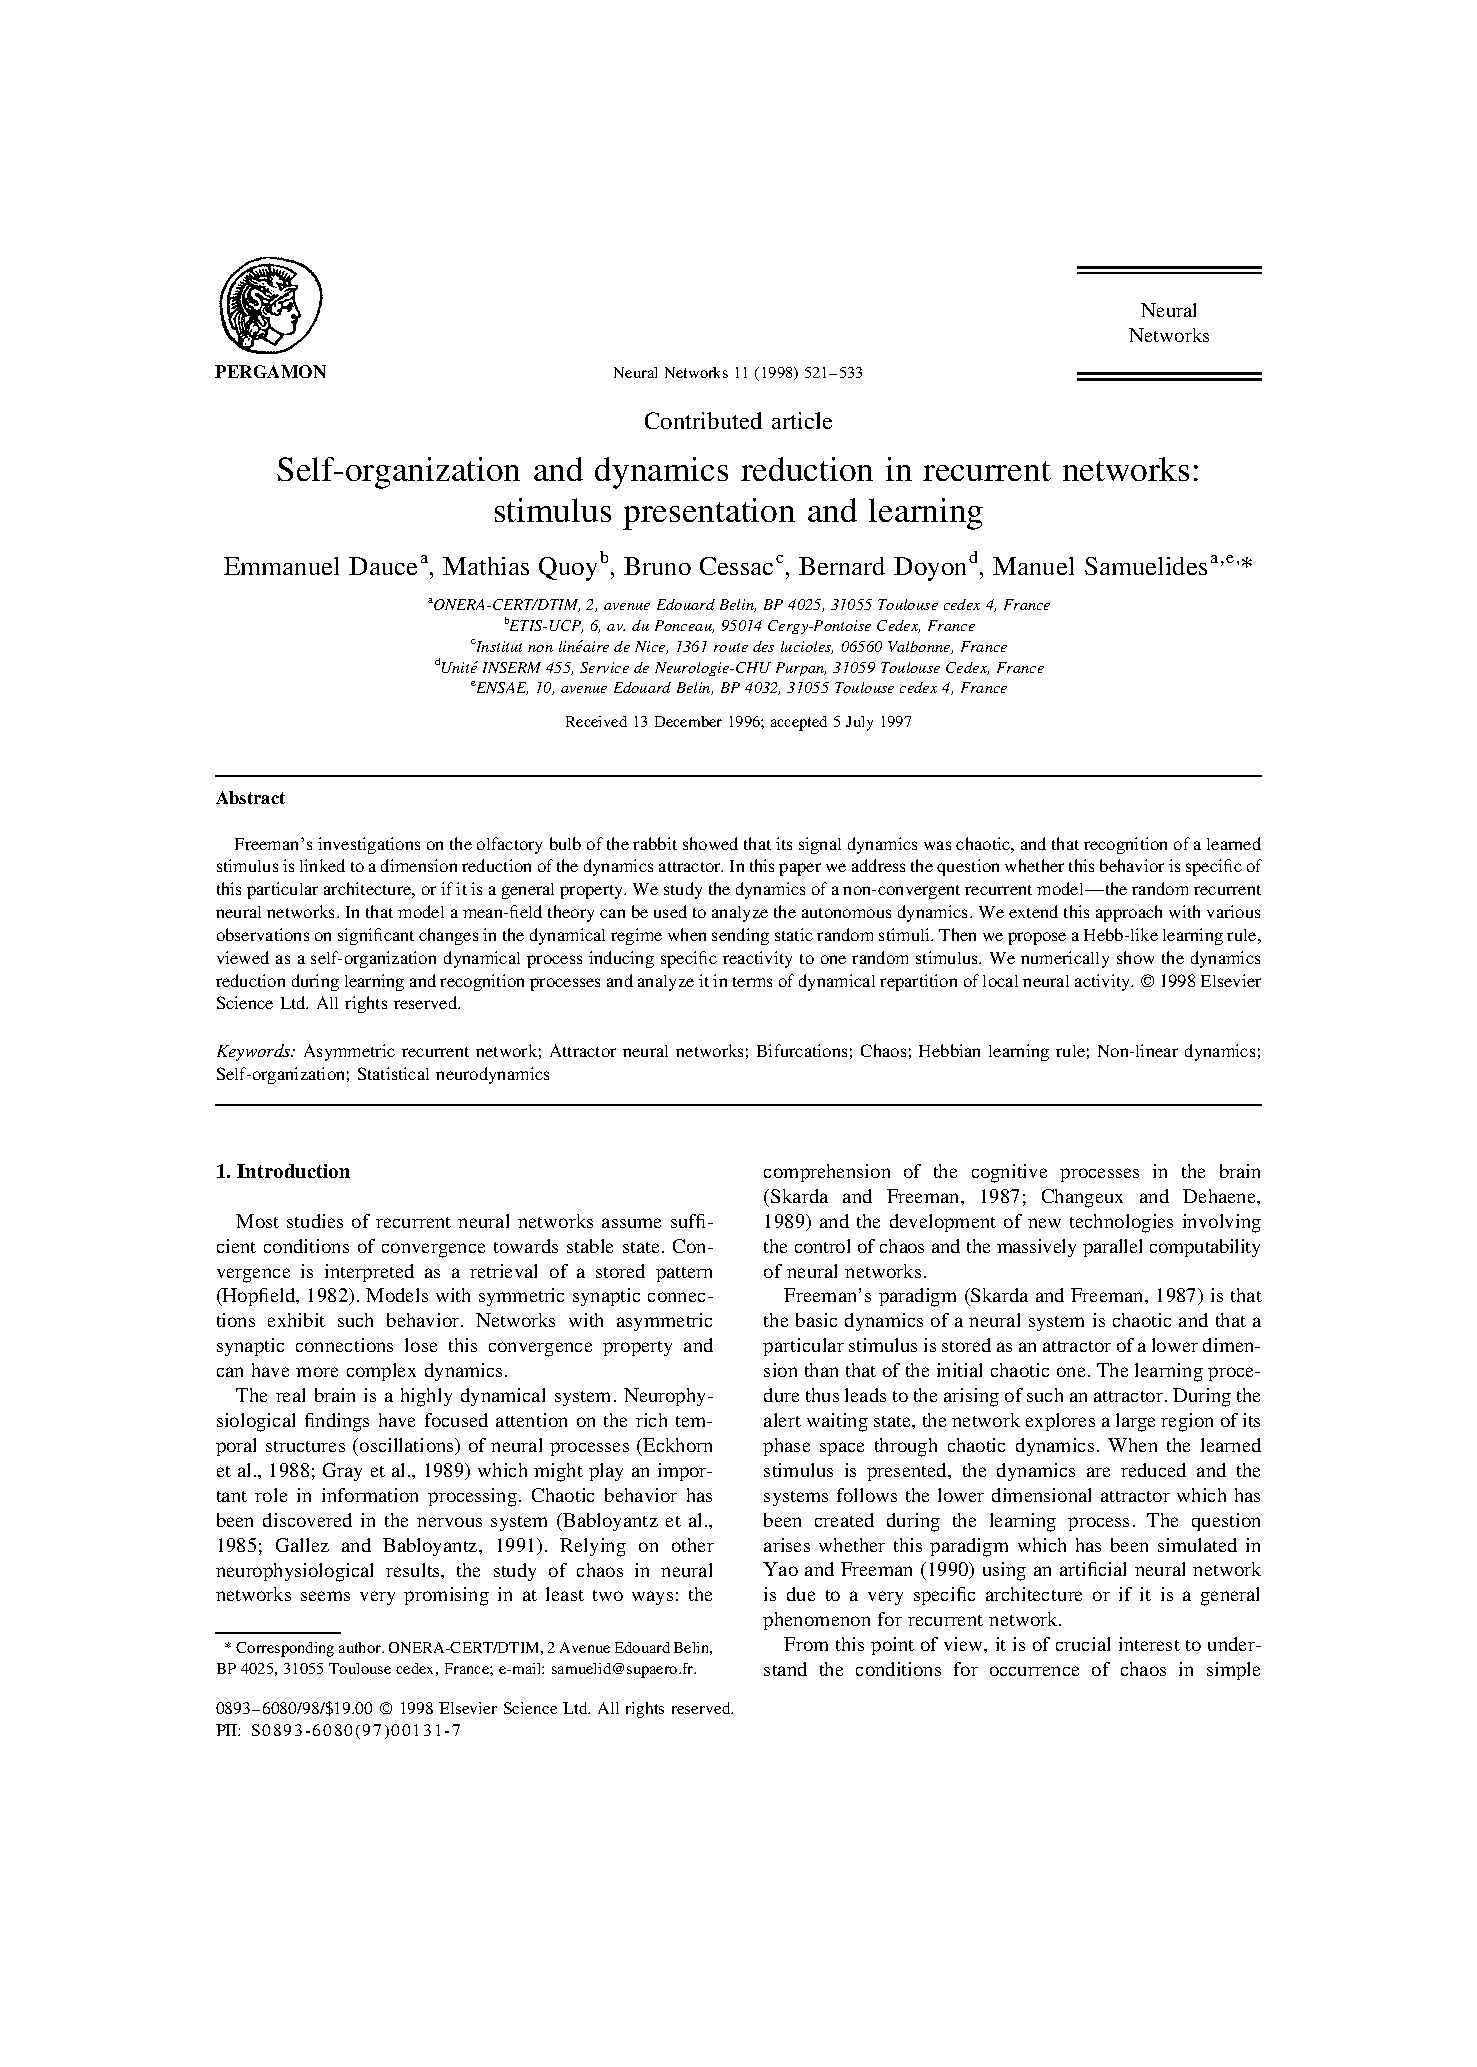
\includepdf[pages=1,offset=50 0]{pdf/1998-neural-networks.pdf}
%\includepdf[pages=2,offset=-65 0]{pdf/1998-neural-networks.pdf}
%\includepdf[pages=3,offset=50 0]{pdf/1998-neural-networks.pdf}
%\includepdf[pages=4,offset=-65 0]{pdf/1998-neural-networks.pdf}
%\includepdf[pages=5,offset=50 0]{pdf/1998-neural-networks.pdf}
%\includepdf[pages=6,offset=-65 0]{pdf/1998-neural-networks.pdf}
%\includepdf[pages=7,offset=50 0]{pdf/1998-neural-networks.pdf}
%\includepdf[pages=8,offset=-65 0]{pdf/1998-neural-networks.pdf}
%\includepdf[pages=9,offset=50 0]{pdf/1998-neural-networks.pdf}
%\includepdf[pages=10,offset=-65 0]{pdf/1998-neural-networks.pdf}
%\includepdf[pages=11,offset=50 0]{pdf/1998-neural-networks.pdf}
%\includepdf[pages=12,offset=-65 0]{pdf/1998-neural-networks.pdf}
%\includepdf[pages=13,offset=50 0]{pdf/1998-neural-networks.pdf}

%\shortcite{Dau98A} {\bf Daucé, E., Quoy, M., Cessac, B., Doyon, B. and Samuelides, M. (1998) Self-organization and dynamics reduction in recurrent networks : stimulus presentation and learning, Neural Network 11:521-533}

%\shortcite{Dau98B} {\bf Daucé E. and Doyon, B. (1998) Novelty Learning in a Discrete Time Chaotic Network, proc. of the 8th International Conference on Artificial Neural Networks (ICANN'98), L. Niklasson et al. eds, Vol. 2: 1051-1056, Springer, September 2-4, Skövde, Sweden}



%- Une méthode d’apprentissage “non-supervisée” (il s’agit de capturer un mode dynamique)

%- mecanisme de base de la route inverse. Notion de “reduction” de la dynamique par apprentissage (baisse de l’impredictibilité, analogie possible avec exploration/exploitation)

%- encodage - patrons statiques - route vers le chaos - destabilisation - frontière du chaos
%}

\cleardoublepage

\subsection{Architectures multi-couches} \label{sec:BioCyb02}

La troisième série de résultats de la thèse et des publication associées \shortcite{Dau00,Dau02} porte sur une architecture 
neuronale  permettant d'implémenter un modèle de la perception des signaux spatio-temporels.
Ces résultats reposent sur une architecture de réseaux récurrents aléatoires à plusieurs couches (deux ou trois).
Le formalisme multi-couches est le même que celui utilisé dans les réseaux équilibrés (voir section \ref{sec:balanced}).
Ici les couches se distinguent non par la nature de leurs neurones mais par le rôle qu'elles prennent dans le processus
d'apprentissage : une (ou deux) couche(s) primaire(s) ayant un rôle passif (sans dynamique intrinsèque)
et une couche secondaire (ou associative) possédant une dynamique intrinsèque, analogue aux réseaux récurrents aléatoires
simples présentés dans la section \ref{sec:NN98}.

Le modèle se présente comme une architecture générique pour l'apprentissage 
de motifs spatio-temporels. 
{\color{Orange} Comme dans le cas précédent, il ne s'agit pas de l'apprentissage d'une réponse 
(d'un read-out) mais d'une modification du comportement du système dynamique en présence
de certains signaux.} La contrainte extérieure se manifeste ici sous
la forme d'un signal spatio-temporel périodique, et la relaxation s'apparente à celle d'un oscillateur
forcé. 
Dans cette étude, comme dans l'étude précédente, l'accent est mis sur la plasticité et l'apprentissage, où 
le comportement ``différent'' est un comportement acquis. 

La règle Hebbienne utilisée est une règle d'ordre 1 (basée sur les différences d'activité), qui
modifie les couplages synaptiques selon une estimation locale de la covariance entre les neurones 
pré et post-synaptiques, en tenant compte du délai de transmission \shortcite{Sej77}. Cette règle, contrairement à la précédente, 
tend à amplifier les variations d'activité. Elle tend asymptotiquement
vers une activité de type cycle limite très robuste à large amplitude individuelle (et non vers un point fixe).
Comme dans le cas précédent, du fait de la non-convergence asymptotique,
la durée d'apprentissage est fixée par l'utilisateur/concepteur
en vue d'optimiser un certain comportement (ici la résonance perceptive). 

Dans la configuration initiale, la couche primaire reçoit passivement le signal spatio-temporel (séquence 
périodique de motifs). Les liens feed-forward aléatoires transmettent ce signal à la couche 
secondaire (dite couche associative). L'activité de la couche associative est un mélange entre cette projection aléatoire
du signal d'entrée et l'activité intrinsèque chaotique (entretenue par les liens latéraux
aléatoires de la couche secondaire). Les liens de feedback (secondaire vers primaire) sont initialement nuls.

La plasticité synaptique a lieu sur deux classes de liens~: latéraux et feedback.  
{\color{Gray} Elle inscrit dans le graphe les 
séquences d'activation prédictibles au sein de l'activité neuronale. }
Outre la réduction de la complexité de l'activité,
la plasticité des liens de feedback crée une boucle d'amplification positive entre la couche associative
et la couche sensorielle, qui transforme la corrélation statistique 
en lien de causalité.
\begin{itemize}
\item L'existence de correspondances statistiques entre l'activité interne et le signal d'entrée produit en effet une amplification du signal d'entrée via cette activité de feedback.
\item Cette projection induite de l'activité interne vers la couche sensorielle
agit comme une prédiction \textit{dans le présent} (voir section \ref{sec:filtrage}), autrement dit fait reposer la connaissance de l'entrée
sensorielle actuelle sur des informations observées dans le passé.
\end{itemize}


{\color{Gray} L'architecture proposée dans \shortcite{Dau02} implémente un principe de traitement
sélectif de la scène sensorielle, en séparant l'espace des sensations entre ce qui est connu (ce qui produit 
un changement qualitatif sous forme de résonance 
perceptive) et ce qui est inconnu (pas de changement qualitatif).
La reconnaissance se traduit par le franchissement d'un seuil (seuil de ``vigilance''),
favorisant le développement d'une activité 
spécifique qui participe à la consolidation et l'entretien de la résonance.}
Le changement par rapport au modèle à une couche réside dans l'utilisation effective des changements qualitatifs 
induits par la plasticité sous la forme du signal de feedback. 
La plasticité permet de \textit{constituer des processus {\color{Orange} attentionnels} spécifiques à certaines configurations
spatio-temporelles apprises}. Ces configurations connues, en activant une résonance, {\color{Orange} révèlent la nature
des connaissance acquises par le réseau.}


Plusieurs papiers de conférences apportent des éclairages complémentaires sur certains aspects du modèle. 
Le papier de la conférence ICANN 2001 \shortcite{Dau01c} présente une version préliminaire du modèle perceptif à deux couches
avec une règle d'apprentissage légèrement plus simple que celle du papier de Biological Cybernetics. 
Le papier de SAB (2000) \shortcite{Dau00b} comporte une partie montrant l'effet de l'apprentissage sur des signaux mixtes composés
d'une partie statique et d'une partie périodique. L'association apprise entre motifs statiques et motifs dynamiques 
se manifeste alors par un niveau de correlation élévé entre la dynamique induite par les motifs mixtes
et la dynamique induite par les motifs statiques seuls (les activités étant par contre qualitativement différentes).

%\cleardoublepage
%\includepdf[pages=1,offset=70 -30]{pdf/2002-biological-cyb.pdf}
%\includepdf[pages=2,offset=-70 -30]{pdf/2002-biological-cyb.pdf}
%\includepdf[pages=3,offset=70 -30]{pdf/2002-biological-cyb.pdf}
%\includepdf[pages=4,offset=-70 -30]{pdf/2002-biological-cyb.pdf}
%\includepdf[pages=5,offset=70 -30]{pdf/2002-biological-cyb.pdf}
%\includepdf[pages=6,offset=-70 -30]{pdf/2002-biological-cyb.pdf}
%\includepdf[pages=7,offset=70 -30]{pdf/2002-biological-cyb.pdf}
%\includepdf[pages=8,offset=-70 -30]{pdf/2002-biological-cyb.pdf}
%\includepdf[pages=9,offset=70 -30]{pdf/2002-biological-cyb.pdf}
%\includepdf[pages=10,offset=-70 -30]{pdf/2002-biological-cyb.pdf}
%\includepdf[pages=11,offset=70 -30]{pdf/2002-biological-cyb.pdf}
%\includepdf[pages=12,offset=-70 -30]{pdf/2002-biological-cyb.pdf}
%\includepdf[pages=13,offset=70 -30]{pdf/2002-biological-cyb.pdf}
%\includepdf[pages=14,offset=-70 -30]{pdf/2002-biological-cyb.pdf}


%{\color{Violet}
%MECANISME DE DESYNCHRO VITAL POU LE FEEDBACK POSITIF. PASSE PAR DES ``CASSURES''.

%Après apprentissage, la séparation de l'espace d'entrée entre
%signaux connus et signaux inconnus passe par la capacité à provoquer une résonance entre 



%NOTION D'ATTRACTEUR / DISCRETISATION / SIMPLIFICATION / CATEGORISATION

%CARACTERE SUPERVISE / NON SUPERVISE ?

%POINT DE VUE COGNITIF

%POINT DE VUE COMPUTATIONNEL


%L'idée d'un feedback positif comme support de la perception n'est pas nouvelle.
%Il a été postulé de longue date comme support des opérations neuronales. 





%{\bf 1999}

%- reseaux à 2 pop : couche primaire et couche secondaire (perceptive).  Mecanisme de “resonance perceptive” (et “resistance au changement”). Importance des delais. 

%- patrons conditionnants (= contexte)

%- règle de covariance - Règle d’ordre 2 (différence-based / covariance rule) 

%{\bf 2000-2001}

%- Perception par feedback positif. Apprentisage “supervisé par la couche primaire”. La couche primaire est à la fois l’entrée et la sortie.

%(Implicitement : 
%(1) Réseau aléatoire avec delais = réservoir de séquences instables dont certaines s’instancient (“emergence”)
%(2) Predictive coding avant l’heure (de type interpolation)
%(3) Controle moteur “supervisé”

%{\bf Daucé, E., Quoy, M. and Doyon, B. (2002) Resonant spatio-temporal learning in large random recurrent networks, Biol.Cybern. 87(3):185-198}

%- implémentation d’un mécanisme de résonance support de la perception et de la mémoire (en particulier generalisation du principe d’interpolation de Hopfield dans le domaine spatio-temporel). Importance des delais dans le traitement temporel.

%- alternances synchronisation (perçu) / non-sens. Système de perception dual. Figure sur fond (Gestalt). 


%}

\cleardoublepage
\subsection{Plasticité dans les réseaux aléatoires équilibrés}

L'étude présentée dans \shortcite{Hen08B} 
est motivée par de nombreuses observations sur le rôle des oscillations 
et de la synchronisation dans le fonctionnement du système nerveux
{\bf!! ref chapitre introduction!!}.
Les réseaux aléatoires équilibrés offrent, comme on l'a vu, la possibilité de développer des régimes 
dynamiques plus variés, permettant en particulier la production d'oscillations synchronisées de
grande amplitude dans certaines configurations.
Il est intéressant dans ce cadre d'étudier comment la plasticité interagit avec la dynamique de population 
pour produire des comportements nouveaux, en particulier des oscillations synchronisées.

Plusieurs indicateurs de complexité ont été mis en place pour mesurer la nature de la dynamique spontanée.
L'analyse du spectre de Fourier ne permet pas d'établir de fréquence caractéristique.
L'autocorrélogramme du signal moyen montre une décroissance exponentielle caractéristique d'un bruit lissé. 
Nous utilisons également un indicateur du nombre de degrés de liberté (basé sur l'ACP \shortcite{wright01}) qui montre
une dimension intrinsèque du signal de l'ordre de 35 pour un réseau de 100 neurones, ce qui indique
une très faible corrélation entre l'activité des différents neurones.
Le réseau développe donc un régime de chaos fort.


L'application de la STDP conduit la dynamique vers   
un régime plus simple. La dimension intrinsèque décroît continument jusqu'à atteindre une valeur faible (entre 2 et 3),
qui caractérise l'entrée dans un régime périodique  \shortcite{Hen08,Hen08B}. Cette
activité périodique est maintenue de manière asymptotique,
ce qui confirme l'appartenance de la STDP aux règles de plasticité d'ordre 1.
La STDP a également un effet régulateur sur le niveau d'activité moyen. Pour
différents taux d'activité individuels initiaux 
(entre 50 et 400 Hz), la STDP conduit le système vers un régime où l'activité individuelle est de l'ordre de 200 Hz.
Le caractère régulateur (homéostatique) de la STDP sur le taux de décharge moyen 
est une caractéristique connue déjà notée par \shortcite{KEMPTER99}.

L'activité finale est caractérisée par une périodicité intrinsèque marquée,
de l'ordre de 20 ms (50 Hz). Cette période correspond à environ deux fois le délai moyen \shortcite{Hen08B},
avec une même séquence d'activation qui se répète en boucle.
L'effet de simplification et de stabilisation d'un régime périodique 
dans les réseaux développant activité intrinsèque a été 
moins souvent noté dans la littérature.
Il semble ici être le résultat de la capture de régularités présentes dans la dynamique initiale,
qui se distingue donc d'un pur processus aléatoire.
La différence entre périodicité globale (50 Hz) et activité individuelle (200 Hz) s'explique par le fait
que les neurones tirent en moyenne quatre fois par cycle.

L'activité périodique finale est une activité très robuste. 
Si l'on interrompt l'apprentissage suffisamment tôt, le comportement du réseau permet de séparer l'activité
induite par le (ou les) motif(s) appris de celle induite par les autres motifs \shortcite{Hen08}. 
En optimisant la durée d'apprentissage, une étude (non publiée) montre
une capacité d'encodage similaire à celle des réseaux continus: le nombre maximal de motifs 
pouvant induire une réponse spécifique est de l'ordre de 5\% du nombre de neurones dans le réseau.

D'un point de vue computationnel, il n'y a qualitativement pas de différence entre le nouveau modèle et
l'ancien. Le comportement induit par la STDP ne semble donc pas reposer sur l'ordre ou 
l'instant de tir des potentiels d'action, mais plutôt sur leur fréquence de décharge.
Cette étude %sur un réseau équilibré
%permet de mettre 
met en évidence un comportement très analogue à celui observé sur le modèle binaire \shortcite{Dau07},
confirmant la parenté fonctionnelle entre la règle TD et la STDP. La STDP est appliquée uniquement sur les connexions 
entre neurones excitateurs. Une convergence vers un régime d'oscillations synchronisées avec une période globales de 
l'ordre de 25 Hz (et une fréquence moyenne individuelle de l'ordre de 200 Hz) est mis en 
évidence. Il s'agit d'une synchronisation observable au niveau de la population, les activités individuelles
restant relativement irrégulières et hétérogènes. Une analyse de la plasticité en fonction des délais met en évidence la potentiation des 
délais longs ($>$ 8 ms) et une dépression des délais intermédiaires (4-8 ms) qui favorise l'entretien du comportement synchronisé (non publié).

%\cleardoublepage
%\includepdf[pages=1,offset=70 -30]{pdf/2008-NEUROCOMP-ann.pdf}
%\includepdf[pages=2,offset=-70 -30]{pdf/2008-NEUROCOMP-ann.pdf}
%\includepdf[pages=3,offset=70 -30]{pdf/2008-NEUROCOMP-ann.pdf}
%\includepdf[pages=4,offset=-70 -30]{pdf/2008-NEUROCOMP-ann.pdf}
%\includepdf[pages=5,offset=70 -30]{pdf/2008-NEUROCOMP-ann.pdf}


\cleardoublepage
\subsection{Plasticité et action de population}

Une dernière étude, publiée récemment dans les proceedings d'ESANN \shortcite{Dau14a}, étudie l'effet de la STDP 
dans un réseau équilibré sous influence d'un signal spatio-temporel. Deux cas sont considérés : signal périodique
(se répétant toutes les 30 ms) ou signal non-périodique. L'activité spontanée sous influence de ces deux types de signaux
est qualitativement la même initialement. La plasticité est appliquée 
dans les deux situations.
Lorsque le stimulus est apériodique, aucun changement qualitatif n'est observé.
Lorsque le stimulus est périodique, l'activité devient plus régulière, avec 
de grandes oscillations (période 16 Hz) observables au niveau de la population.
Le comportement est assez proche du comportement de grandes oscillations lentes
obtenu sous influence statique. On observe 
néanmoins une synchronisation des oscillations du réseau avec la période 
du stimulus, autrement dit il y a un accrochage de phase de sorte que la période interne (60 ms)
est exactement le double de la période du signal (30 ms). Ce comportement d'accrochage est assez comparable
à celui observé sur les réseaux plus simples. Le réseau devient ``réactif'' aux motifs périodiques appris,
développant une ``action de population'' qui est un analogue global des potentiels
d'action neuronaux.
%
%\cleardoublepage
%\includepdf[pages=1-2,landscape=true,nup=1x2,scale=1.1,offset= 80 -30]{pdf/2014-esann-A-ann.pdf}
%\includepdf[pages=3-4,landscape=true,nup=1x2,scale=1.1,offset= -80 -30]{pdf/2014-esann-A-ann.pdf}
%\includepdf[pages=5-6,landscape=true,nup=1x2,scale=1.1,offset= 80 -30]{pdf/2014-esann-A-ann.pdf}

%{\color{Violet}
%Fred Henry : Master en 2005.

%bourse these : 
%juin 2005 Ste Marguerite (initiation de neurocomp)

%These Fred : pb : le lien avec le mouvement?

%* 2005-2006 * 

%oct. 2005 NOLTA - 

%jan 2006 institut H Poincaré - 

%juillet 2006 CNS à Edinbourg (modèle Gaussien du Master)

%* 2006-2007 *

%Dyva en sept 2006 présenté par Fred - idées orientées neural field + colliculus + LIF simple

%oct. 2006 premiere conf. Neurocomp - 
%idées RL + couche récurrente intermédiaire. 
%Policy Gradient (Bartlett) = local changes = Hebb/anti-Hebb
%Idée d'interversion bruit/signal dans les modèles à 2 couches (Gaussiennes centrées?).
%Illustration avec simu Khepera.

%juin 2007 - NIPS (refusé). 
%modèle LIF/SRM à courant (avec free mb. potential h). 
%- Connexions gaussiennes centrées . DELAI FIXE (10 ms)
%STDP --> activité périodique non synchronisée

%papier EPJ-ST : modèle RL Hebb/anti-Hebb avec terme (1-H) (comme SAB) sur liens excitateurs - separation exc/inh.

%* 2007-2008 *  

%Dyva en sept 2007 (signé Daucé) - poursuite approche RL-PG appliquée aux saccades.
%(Fred ne participe pas à ce projet)

%ESANN avril 2008 : idem NIPS sauf DELAI VARIABLE (Poisson moy. 10 ms). STDP produit oscillations lentes. entrée = POTENTIEL.

%Tentative publi dans neurocomputing - echec. (calcul plus fin de la ``loading capacity'' - !! sur ordi Centrale only)

%* ATER Lille 2008-2009 *

%oct. 2008 - 2eme Neurocomp. Distinction input courant/input potentiel. differents regimes sont obtenus selon le type
%d'input / les parametres internes.

%juillet 2009 : CNS - séparation excitateurs/inhib. Plasticité sur exc. seulement. delais variables. effet 
%stdp sur delais.

%septembre 2009 : suite projet RL. 

%ACI 'temps et cerveau' va de 2002 à 2007 (5 ans???)

%MAPS commence en septembre 2007 (le dossier a été monté en janvier-février 2007)


%{\bf 2008}
%- modèles à 2 couches (strictly excitatory/inhibitory). 

%{\bf 2009}

%- “Free membr. potential” (synaptic input) / modeles ECM à “horizon fini” 

%Mean field

%Mon apport :
%- Multi-pop
%- Délais
%- frontiere
%- contrib. Reseaux equilibrés --> comportementdes réseaux équilibrés à la frontière

%On-off states?



%{\bf 2008}

%- Balanced networks et STDP.

%{\bf 2014}

%- population response (population “spike”) avec STDP. Importance des termes de reequilibrage des poids et de la SFA.  Idée de multi-échelle et de detecteur d’information mutuelle à travers l’activité. Idée de STDP comme sequence enhancement.

%UP/DOWN

%Brunel

%Frequences, rythmes, periodicités


%}

%%%%%%%%%%%%%%%%%%%%%%%%%%%%%%%%%%%%%%%%%%%%%%%%%%%%%%%%%%%%%%%%%%%%%%%%%%%%%%%%%%%%%%%%%%%%%%%%%%%%%%%%%%%%%%%%%%%
%%%%%%%%%%%%%%%%%%%%%%%%%%%%%%%%%%%%%%%%%     2.4      %%%%%%%%%%%%%%%%%%%%%%%%%%%%%%%%%%%%%%%%%%%%%%%%%%%%%%%%%%%%
%%%%%%%%%%%%%%%%%%%%%%%%%%%%%%%%%%%%%%%%%%%%%%%%%%%%%%%%%%%%%%%%%%%%%%%%%%%%%%%%%%%%%%%%%%%%%%%%%%%%%%%%%%%%%%%%%%%
\cleardoublepage
\subsection{Discrimination de séquences spatio-temporelles}

Les protocoles d'apprentissage présentés jusqu'à présent avaient pour but de 
former une réponse induite. La forme de la réponse n'était pas 
fixée à priori et dépendait des caractéristiques du substrat.
Il n'y avait pas de ``read-out'', il s'agissait juste de produire une dynamique de relaxation qui se 
conforme à (prenne forme avec) la contrainte imposée, en rendant le réseau plus réactif à certains 
motifs présentés.


Nous considérons ici une architecture 
à entrées-sorties complète.
Le réseau possède une couche d'entrée qui 
transmet passivement le signal, une couche récurrente aléatoire, et une couche de sortie
constituée dans ce cas de quelques neurones dont la sortie est lue.
La forme de la réponse induite est imposée par l'expérimentateur,
de manière supervisée ou semi-supervisée.

La tâche consiste à discriminer quatre motifs spatio-temporels.
Ces motifs possèdent des éléments en communs, de telles sorte qu'il est impossible de séparer les signaux
sur la base de l'entrée instantanée.
Chaque neurone de sortie représente une catégorie.
La réponse est fixée par le neurone qui émet le premier potentiel d'action suite
à la présentation du motif.

Le protocole d'apprentissage consiste à présenter les séquences périodiquement, 
lire les réponses produites, informer le réseau du caractère correct ou incorrect de sa
réponse et appliquer une règle de plasticité visant à augmenter le taux de réponses correctes, selon
un principe qui se rapproche de l'apprentissage par renforcement.

L'apprentissage utilise sur les effets symétriques des règles Hebbienne et anti-Hebbienne 
sur la dynamique des réseaux récurrents aléatoires, montrés dans \shortcite{dauce05}.
Par exemple, l'anti-STDP (règle miroir de la STDP) a pour effet d'augmenter la complexité
de la dynamique intrinsèque, soit un effet contraire à la STDP. L'application successive
de la STDP puis de l'anti-STDP sur un réseau récurrent aléatoire 
a pour effet de réduire la complexité puis de l'augmenter à nouveau.

L'étude est également une implémentation originale du codage par rang, utilisant un principe 
concurrent d'avance vs. retard de la réponse.
Si la réponse est correcte, la STDP est appliquée sur la couche de sortie et sur la couche récurrente,
ce qui tend à anticiper l'instant de réponse du neurone ayant tiré.
Si la réponse est incorrecte, c'est l'anti-STDP qui est appliquée, 
tendant à retarder la réponse.
Le papier \shortcite{henry07} utilise des signaux temporels très lents, où
la séquence est composée de 4 motifs durant chacun 100 ms, de sorte qu'une séquence
complète dure 400 ms. Dans ce cas, le temps nécessaire pour atteindre des taux
de réussite raisonnables s'exprime en heures (environ 100000 essais).
Les résultats présentés dans \shortcite{Dau06} utilisent des séquences plus courtes (40 ms).
Dans ce cas, environ 500 essais suffisent pour obtenir une discrimination parfaite.

La différence de taux d'apprentissage et de taux de réussite s'explique principalement par 
la différence d'échelle temporelle des séquences à apprendre. La mémoire d'une unité neuronale est de l'ordre de
sa constante de membrane, soit 10 à 20 ms.
Néanmoins, à la
lumière des résultats du chapitre précédent, la plasticité semble 
capable d'induire suffisamment de régularité dans la dynamique intrinsèque
pour conserver une mémoire plus importante 
au sein de la population. La difficulté à discriminer les séquences de 400 ms semble
néanmoins fixer la limite supérieure de cette capacité (100 ms étant en pratique suffisant 
pour discriminer deux séquences).

%\cleardoublepage
%\includepdf[pages=1,offset=70 -30]{pdf/2007-neurocomputing.pdf}
%\includepdf[pages=2,offset=-70 -30]{pdf/2007-neurocomputing.pdf}
%\includepdf[pages=3,offset=70 -30]{pdf/2007-neurocomputing.pdf}
%\includepdf[pages=4,offset=-70 -30]{pdf/2007-neurocomputing.pdf}
%\includepdf[pages=5,offset=70 -30]{pdf/2007-neurocomputing.pdf}
%\includepdf[pages=6,offset=-70 -30]{pdf/2007-neurocomputing.pdf}
%\includepdf[pages=7,offset=70 -30]{pdf/2007-neurocomputing.pdf}
%\includepdf[pages=8,offset=-70 -30]{pdf/2007-neurocomputing.pdf}

%{\color{Violet}
%{\bf 2005}



\chapter{Architectures de contrôle}

{\color{Cyan} 

\begin{itemize}	
\item Langage de l'action. 

\item Espace de la tâche. Passage d'échelle et variable d'ordre.

\item Scène sensorielle et scène motrice

\item Facteurs causaux.

\item La tâche. L'espace de la tâche (Marr) = niveau computationnel.

\end{itemize}
}

\section{Notions générales}

{\color{Cyan} Cette section présente un formalisme et des définitions visant à ...}

\subsection{Contrôleur et environnement}

L'approche dite ``située'' en robotique
mobile et en intelligence artificielle \shortcite{Bro91,Varela91} prône la prise 
en compte de la contrainte du corps
comme élément structurant du développement de {\color{Orange} capacités cognitives} plus élaborées.
{\color{Orange} Cette contrainte, qui s'exprime par les {\bf dépendances sensori-motrices}, et 
la prise en compte des {\bf disparités d'échelle}, augmente néanmoins considérablement 
la complexité des tâches
d'apprentissage et de leur implémentation par plasticité synaptique. }

Le cadre que nous considérons ici est celui de la commande motrice. Nous considérons un programme doté d'effecteurs moteurs capables de déplacer et faire pivoter des masses articulées dans l'espace physique.  L'espace physique est décrit, d'une part, par ces effecteurs directement contrôlables, ainsi que d'autres éléments physiques non directement contrôlables. 
\begin{itemize}
	\item Le programme est le \textit{contrôleur}.
	\item L'espace physique est l'\textit{environnement}.
\end{itemize}  

L'interaction d'un contrôleur avec son environnement passe par des transducteurs, qui sont les canaux de 
communication entre les deux milieux~:
appareils sensoriels et proprioceptifs chez les animaux, et contractions musculaires permettant de déplacer des masses
articulées; senseurs et actuateurs pour les dispositifs de contrôle artificiels : capteurs qui traduisent des signaux physiques
en signaux électriques, moteurs, joints et pistons pour les déplacements de masses.


Le cadre que nous avons regardé jusqu'à présent est l'apprentissage en ``boucle ouverte'',
dans lequel les actions physiques sur le milieu sont découplées des sensations. 
{\color{Gray} C'est le cadre classique du conditionnement Pavlovien où les stimuli déclenchent
des réponses comportementales automatiques ou induites par l'apprentissage.}
La prise en compte plus réaliste
des deux domaines matériels que sont le circuit logiciel et le milieu physique
environnant conduit à déplacer 
le cadre conceptuel de l'apprentissage vers l'apprentissage en ``boucle fermée''.
Il se définit formellement par la présence de corrélations entre les actions ou 
les réponses produites et les manifestations sensorielles suivantes.


\subsubsection{Couplages sensori-moteurs}
Ce lien entre les actions et les sensations est décrit, au niveau le plus général, par le modèle physique 
au sein duquel le logiciel est plongé.

Nous reprenons ici le formalisme des systèmes dynamiques proposé dans l'équation (\ref{eq:SD}). On suppose que le milieu physique et le programme obéissent à une description d'état, où 
\begin{itemize}
	\item $\boldsymbol{x}_\text{out}$ est un vecteur d'état  décrivant le milieu physique (actuateurs compris)
	\item $\boldsymbol{x}_\text{in}$ est un vecteur d'état  décrivant le contrôleur \--- ou encore ``milieu'' logiciel (entrées sensorielles comprises).
\end{itemize}

L'évolution du système au cours du temps est alors décrite par le jeu d'équations~:
\begin{align}
&\boldsymbol{x}_\text{out}' = \phi_\text{out}(\boldsymbol{x}_\text{out},h_\text{out}(\boldsymbol{x}_\text{in})) \label{eq:SD-closed-out}\\
&\boldsymbol{x}_\text{in}' = \phi_\text{in}(\boldsymbol{x}_\text{in},h_\text{in}(\boldsymbol{x}_\text{out})) \label{eq:SD-closed-in}
\end{align}
où $h_\text{in}$ et $h_\text{out}$ représentent (de manière simplifiée) les mécanismes de transduction entre le milieu physique et le circuit logiciel  et $\phi_\text{in}$ et $\phi_\text{out}$ les fonctions d'évolution d'état.

Plus précisément~:
\begin{itemize}
	\item $\boldsymbol{I}(t) = h_\text{in}(\boldsymbol{x}_\text{out}(t))$ est le signal d'entrée du contrôleur.
	\item $\boldsymbol{u}(t) = h_\text{out}(\boldsymbol{x}_\text{in}(t))$ est la commande motrice.
	\item L'équation (\ref{eq:SD-closed-out}) décrit le lien entre les actions produites et les sensations.
	\item L'équation (\ref{eq:SD-closed-in}) décrit le traitement appliqué à l'entrée sensorielle.
\end{itemize}
\paragraph {Remarques~:}
\begin{enumerate}
	\item L'état de l'environnement n'est connu du contrôleur qu'à travers une projection $h_\text{in}$ qui n'est pas nécessairement inversible. On dit dans ce cas que l'environnement (ou une partie de l'environnement) est ``caché''.
	\item 	La simplification, qui consiste à considérer un milieu intérieur (intensif) et un milieu extérieur (extensif)
	couplés comme un seul et même système dynamique, se
	heurte souvent au caractère inhomogène de ce couplage~:
	\begin{itemize}  
		\item Dans domaine biologique, les échelles de temps et d'espace des comportements macroscopiques 
	(mouvements, déplacements, activité motrice)  
	se distinguent des échelles de temps et d'espace observées au niveau de l'activité
	nerveuse.
	Les actions produites par le corps sont à une échelle temporelle lente en comparaison des potentiels d'action
	produits par les neurones. On parle de \textit{Disparité d'échelle}.
		\item 
	En plus de la disparité d'échelle, les lois régissant les deux systèmes ne sont pas de même nature. 
	Le monde physique est assez bien décrit par 
	l'approximation newtonienne des masses en mouvement dans un milieu tri-dimensionnel.
	%On parlera pour simplifier du milieu extensif pour désigner le monde physique, l'endroit où sont
	%possibles des déplacements de masses par l'action des forces, les frottements et le contact. 
	A l'inverse, l'activité logicielle s'inscrit dans un réseau où l'intensité des interactions est 
	faiblement liée à la disposition spatiale, essentiellement produite par la connectique et 
	les transports d'activité électrique.
	%On parle pour simplifier de milieu intensif. % (ou milieu logiciel).
	\end{itemize}
    \item {\color{Cyan} On peut compléter l'équation de manière symétrique avec une plasticité de l'environnement représentant la non-stationnarité, l'usure, le vieillissement et toutes sortes de changement ``lents''.}
\end{enumerate}
	
 	
 Le contrôle en boucle fermée \cite{Wiener1965}
 consiste à programmer le contrôleur de telle sorte que les actions produites dans le milieu se conforment à un certain nombre de critères (ou contraintes) définis \textit{a priori}.	
 Ces critères peuvent être :
 \begin{itemize}
 	\item le caractère non délétère des actions produites (endommagement du dispositif moteur ou de l'environnement)
 	\item la minimisation de certaine dépenses (consommation énergétique, effort, usure, chauffage des composants, ...)
 	\item la rapidité de la réponse
 	\item la résilience, la capacité à résister aux perturbations (homéostasie)
 	\item la stabilité et la reproductibilité des réponses, la robustesse.
 	\item etc. 
 \end{itemize}

Ces problèmes ont été analysés de longue date dans le cadre de la théorie de l'automatique (contrôle linéaire) et de la commande optimale, en particulier sous l'angle de la stabilité de la réponse à la commande et de l'homéostasie {\color{Orange}[REFS]}.

\subsubsection{Tâches et problèmes de contrôle}

La théorie du contrôle classique décrit un problème de contrôle comme un problème d'optimisation basé sur~:
\begin{itemize}
	\item une consigne, correspondant à un état nominal $\boldsymbol{x}^*$ dans lequel on souhaite voir le milieu physique,
	\item un contrôleur doté de capteurs et d'actuateurs,
	\item et le milieu physique situé dans l'état $\boldsymbol{x}_\text{out}$.
\end{itemize}

Le problème d'optimisation consiste à programmer une fonction de réponse $\phi_\text{in}$ qui, étant donnée une consigne $\boldsymbol{x}^* \in \mathcal{C}$, conduit le milieu physique dans l'état désiré. 


{\bf Exemple~}: Dans le cas d'un bras mécanique, $\boldsymbol{x}_\text{out}$ peut décrire les coordonnées spatiales d'un effecteur et $\boldsymbol{x}^*$ la position finale désirée.

{	\color{Gray}Dans le cadre de problèmes de robotique, on distingue généralement~: 
	\begin{itemize}
		\item l'espace de la tâche (par exemple atteindre une certaine position de l'espace  avec l'extrémité du bras)
		\item et l'espace des articulations, décrivant le détail des positions des éléments mécaniques composant le robot.
	\end{itemize}	
	Pour une position finale unique, il existe en général plusieurs configurations des articulations. 
}
	
\paragraph{}


\subsubsection{Erreur motrice et erreur de prédiction}
 La différence $\boldsymbol{x}^* - \boldsymbol{x}_\text{out}(t)$ est appelée l'\textit{erreur motrice}.

 Le principe de contrôle le plus élémentaire  correspond à une commande directement proportionnelle à l'erreur motrice, autrement dit $\boldsymbol{u}(t) \propto \boldsymbol{x}^* - \boldsymbol{x}_\text{out}(t)$. En tenant compte de l'inertie et des temps de réponse, il permet d'obtenir un contrôleur homéostatique stable  (résistant aux perturbations). 
 
 
Le cas le plus courant en robotique et en modélisation biologiquement inspirée correspond néanmoins à une situation où l'erreur motrice n'est pas directement observable. Deux cas se présentent~: 
\begin{enumerate}
	\item $\boldsymbol{I}= h_\text{in}(\boldsymbol{x}_\text{out})$ est le signal issu des appareils de mesure. Le contrôleur doit, autant que possible, deviner la valeur de l'état, soit $\tilde{\boldsymbol{x}} \simeq h_\text{in}^{-1}(\boldsymbol{I})$ pour produire la commande. On parle de \textit{modèle inverse}.
	\item Une autre approche consiste à comparer le signal observé au signal attendu  $\boldsymbol{I}^* = h_\text{in}(\boldsymbol{x}^*)$. Ce signal attendu n'est pas directement observable. Il peut être \textit{reconstruit} via un \textit{modèle direct}. 
	\begin{itemize}
		\item On dit que le modèle effectue une prédiction sensorielle et la différence entre l'entrée prédite et l'entrée attendue est l'\textit{erreur de prédiction}.
		\item La sortie motrice doit être telle que cette erreur de prédiction sensorielle soit minimisée.
	\end{itemize}
\end{enumerate}

\paragraph{Remarque~:} Il est possible d'établir une analogie entre consigne et programme. Une consigne s'apparente plus précisément à un \textit{programme moteur} qui conditionne la manière dont le contrôleur traite ses entrées sensorielles~: pour deux consignes différentes, les mêmes entrées sensorielles ne produisent pas la même réponse.  

\subsubsection{Facteurs exogènes}

Le problème de l'observation de l'état est donc d'une importance particulière en contrôle puisque la justesse de la commande en dépend. 

L'estimation d’état dépend principalement de deux facteurs: le modèle physico-mécanique de l'environnement, et le modèle des capteurs. 
Ces modèles sont souvent incomplets  et les facteurs non pris en compte (frottements, inertie, fatigue des composants, non-stationnarités, variations d'éclairage, bruit de mesure, fiabilité des capteurs, ...) sont modélisés comme des signaux extérieurs venant moduler de façon imprévisible le comportement du système. 
 
Ces facteurs exogènes sont modélisés comme des signaux
venant influencer le système, mais n'étant pas influencés par lui.   
L'équation de mise à jour devient~:
\begin{align}
&\boldsymbol{x}_\text{out}' = \phi_\text{out}(\boldsymbol{x}_\text{out},\boldsymbol{u},\boldsymbol{\xi}_\text{out}) \label{eq:feed-noise-1} \\
&\boldsymbol{I} = h_\text{in}(\boldsymbol{x}_\text{out},\boldsymbol{\chi}_\text{out}) \label{eq:feed-noise-2}\\
&\boldsymbol{x}_\text{in}' = \phi_\text{in}(\boldsymbol{x}_\text{in},\boldsymbol{I},\boldsymbol{\xi}_\text{in}) \label{eq:feed-noise-3} \\
&\boldsymbol{u} = h_\text{out}(\boldsymbol{x}_\text{in},\boldsymbol{\chi}_\text{in}) \label{eq:feed-noise-4}
\end{align}
où les entrées $\boldsymbol{\xi}_\text{out}(t)$, $\boldsymbol{\chi}_\text{out}(t)$, $\boldsymbol{\xi}_\text{in}(t)$, $\boldsymbol{\chi}_\text{in}(t)$ représentent les écarts entre le modèle et la ``réalité''. 


\subsection{Approche probabiliste}

Les écarts entre le modèle et les observations sont fréquemment modélisés comme des \textit{bruits}, issus de tirages aléatoires indépendant de la dynamique d'état, où~:
\begin{itemize}
	\item  %$\boldsymbol{\xi}_\text{in}(t)$ et
	 $\boldsymbol{\xi}_\text{out}(t)$ est le bruit d'état et $P$ le modèle de transition d'état externe, selon~:
	 \begin{align}\boldsymbol{x}_\text{out}(t+dt)\sim P(\boldsymbol{X}|\boldsymbol{x}_\text{out}(t),\boldsymbol{u}(t))
	 \end{align}
	\item  %$\boldsymbol{\chi}_\text{in}(t)$ et
	 $\boldsymbol{\chi}_\text{out}(t)$ est le bruit de mesure et $Q$ le modèle de mesure, selon~:
	 \begin{align}
	 \boldsymbol{I}(t)\sim Q(\mathcal{I}|\boldsymbol{x}_\text{out}(t))
	 \end{align}
\end{itemize}  
Les équations (\ref{eq:feed-noise-1}-\ref{eq:feed-noise-4}) décrivent alors la réalisation d'un processus stochastique reposant sur, d'une part, des modèles d'état (les variables ``porteuses'' de signal \--- ou d'information) et d'autre part des modèles de bruit (variables ``porteuses'' de bruit).

Étant donné l'état connu $\boldsymbol{x}_\text{out}(t)$, l'estimation d'état suivant peut être produite à l'aide de la formule de Bayes~:
\begin{align}\label{eq:bayes}
\mathbb{P}(\boldsymbol{x}|\boldsymbol{I}(t+dt)) = \frac{P(\boldsymbol{x}|\boldsymbol{x}_\text{out}(t),\boldsymbol{u}(t)) Q(\boldsymbol{I}(t+dt)|\boldsymbol{x})}{\int_{\mathcal{X}}P(\boldsymbol{y}|\boldsymbol{x}_\text{out}(t),\boldsymbol{u}(t)) Q(\boldsymbol{I}(t+dt)|\boldsymbol{y})d\boldsymbol{y}}
\end{align}  
où~:
\begin{itemize}
	\item $P(\boldsymbol{x}|\boldsymbol{x}_\text{out}(t),\boldsymbol{u}(t))$ est la probabilité \textit{a priori}.
	\item  $Q(\boldsymbol{I}(t+dt)|\boldsymbol{x})$ est la vraisemblance de l'observation $\boldsymbol{I}$ étant donné $\boldsymbol{x}$. 
\end{itemize}

\subsubsection{Filtrage}

Le problème de filtrage consiste principalement à séparer le signal du bruit, à l'aide de la connaissance (ou \textit{a priori}) représentée par les modèles d'état et les modèles de bruit.

Soit $\boldsymbol{I}(t)$ le signal disponible sur les capteurs. Il s'agit d'estimer le mieux possible l'état extérieur \--- ou état ``caché'' $\boldsymbol{x}_\text{out}(t)$. Autrement dit il s'agit de soustraire du signal les bruits ($\boldsymbol{\xi}_\text{out}(t), \boldsymbol{\chi}_\text{out}(t)$), connaissant leurs caractéristiques statistiques.

Le filtrage utilise un \textit{modèle interne}, qui est un processus miroir de l'environnement, dans lequel la variable d'état \textit{interne} $\boldsymbol{x}_\text{in}$ évolue en ``imitant'' l'environnement. On note dans ce cas $\hat{\boldsymbol{x}}_\text{out}=\boldsymbol{x}_\text{in}$ cette estimation, sur laquelle le contrôleur s'appuie pour choisir sa commande.



Le problème est principalement celui de compenser la dérive de l'estimation d'état dans le cas de processus aléatoires avec bruit additif (cas où l'écart à la moyenne augmente au cours du temps). 
Il s'agit donc de produire la meilleure estimation \textit{à chaque instant} de l'état extérieur $\hat{\boldsymbol{x}}_\text{out}(t+dt)$.


\paragraph{Dynamique interne} 
Dans le cadre des modèles de filtrage, l'état interne tel que défini dans l'équation (\ref{eq:SD-closed-in}) est le résultat d'un processus \textit{récurrent} reposant
\begin{itemize} 
	\item sur des facteurs internes représentés par la probabilité a priori 
$P(\boldsymbol{x}_{t+1}|\boldsymbol{x}_t,\boldsymbol{u}_t)$ 
	\item sur des facteurs externes représentés par la vraisemblance $ Q(\boldsymbol{I}_t|\boldsymbol{x}_t)$
\end{itemize}
où les indices représentent le temps en notation discrète.

L'évolution de l'état repose sur a formule de Bayes (\ref{eq:bayes}), soit le maximum a posteriori en tenant compte des estimations précédentes.  En prenant en compte les deux critères, on peut définir une dynamique sur la distribution comme~:
\begin{align}
& f(\hat{\boldsymbol{x}}_0) = f_0(\hat{\boldsymbol{x}}_0)\\
& g(\hat{\boldsymbol{x}}_{t+1}|\hat{\boldsymbol{x}}_{0:t},\boldsymbol{I}_{1:t},\boldsymbol{u}_{1:t}) \propto P(\hat{\boldsymbol{x}}_{t+1}|\hat{\boldsymbol{x}}_t,\boldsymbol{u}_t) f(\hat{\boldsymbol{x}}_t|\hat{\boldsymbol{x}}_{0:t-1},\boldsymbol{I}_{1:t},\boldsymbol{u}_{1:t-1}) \label{eq:accum-1} \\
& f(\hat{\boldsymbol{x}}_{t+1}|\hat{\boldsymbol{x}}_{0:t},\boldsymbol{I}_{1:t+1},\boldsymbol{u}_{1:t}) \propto
Q(\boldsymbol{I}_{t+1}|\hat{\boldsymbol{x}}_{t+1}) g(\hat{\boldsymbol{x}}_{t+1}|\hat{\boldsymbol{x}}_{0:t},\boldsymbol{I}_{1:t},\boldsymbol{u}_{1:t})  \label{eq:accum-2}
\end{align}
où les termes de normalisation ont été omis, avec  $\hat{\boldsymbol{x}}_{0:t}$ représentant une trajectoire particulière du processus stochastique et les densités de probabilité $f$ et $g$ portent sur l'espace d'états $\mathcal{X}$ du processus externe.
 
Le jeu d'équations (\ref{eq:accum-1}-\ref{eq:accum-2}) forme une équation d'\textit{observation} où la nouvelle estimation  $f(\hat{\boldsymbol{x}}_{t+1}|\hat{\boldsymbol{x}}_{0:t},\boldsymbol{I}_{1:t+1},\boldsymbol{u}_{1:t})$ se déduit de l'estimation précédente $f(\hat{\boldsymbol{x}}_t|\hat{\boldsymbol{x}}_{0:t-1},\boldsymbol{I}_{1:t},\boldsymbol{u}_{1:t-1})$ et de l'observation des nouveaux signaux $\boldsymbol{u}_t$ et $\boldsymbol{I}_{t+1}$. L'espace $\mathcal{X}$ est appelé l'espace des \textit{sources} de l'observation.

\paragraph{Erreur de prédiction}
L'équation (\ref{eq:accum-1}) représente la première étape de l'estimation aboutissant à une prédiction ``interne''  sur l'espace des sources. Cette prédiction est combinée (eq. \ref{eq:accum-2}) à la vraisemblance $Q$ , qui peut être vue comme une prédiction ``inverse'' sur l'espace des sources. 
L'écart entre les deux distributions est l'\textit{erreur de prédiction}, également appelée \textit{innovation} \cite{Kalman1960}. Les différences de variance entre les distributions permettent de privilégier l'un ou l'autre selon que le bruit d'état ou le bruit de mesure dominent le processus d'observation.

\paragraph{Remarques~:}
\begin{itemize}
	\item Pour des raisons de précision numérique, il est fréquent d'utiliser des logarithme de probabilités au lieu des probabilités elles-mêmes (le produit étant ``remplacé'' par une somme).
%	\item Dans le cas de modélisation par processus gaussiens, {\color{Orange} le produit de deux  gaussiennes est une gaussienne }. L'équation d'évolution est remplacée par l'évolution des paramètres de la distribution (moyenne et matrice de variance-covariance). Les modèles de filtrage classique 
%	utilisent l'erreur de {\color{Orange} prédiction sensorielle -- ou prédiction dans l'espace d'état?? (ou ``innovation'') $\boldsymbol{e}_\text{in}(t+dt)=\boldsymbol{I}(t+dt) - h_\text{in}(\boldsymbol{x}'_\text{out}(t+dt))$ pour corriger la prédiction interne. A REPRENDRE}

	\item Un cas particulier important est le modèle sans transition d'état ($\forall t, \boldsymbol{x}_{\text{out}}(t) = \boldsymbol{x}_\text{out}$). Ce cas correspond à des mesures bruitées multiples opérées sur les mêmes données. Le fait de multiplier les observations permet de réduire à chaque mesure l'incertitude sur l'état ``réel'' observé. Ce mécanisme, est appelé d'\textit{accumulation d'évidence}. Dans le cadre de campagnes de mesures, il permet de décider à chaque mesure s'il est nécessaire ou pas d'en effectuer une nouvelle, en fonction d'un seuil de fiabilité fixé \cite{Wald47}.
\end{itemize}

\paragraph{Exemples}~:
\begin{itemize}
	\item Le filtre de Kalman \shortcite{Kalman1960} utilise des modèles de bruit gaussiens, définis par une moyenne et une matrice de variance-covariance. L'environnement est modélisé comme un processus gaussien soumis à une commande extérieure connue.
	\item Les modèles de chaines de Markov cachés \shortcite{Baum1966} utilisent une représentaton d'état discrète. L'environnement est  une chaîne de Markov connue. Chaque état de la chaîne génère une mesure selon une distribution connue. Le problème consiste principalement, à partir de la mesure, à identifier les transitions d'état (algorithmes forward-backward, de Viterbi,...).   
	\item Les filtres particulaires \shortcite{Doucet2001} utilisent une approche de Monte Carlo pour échantillonner l'espace d'état du processus externe à chaque instant. Chaque ``particule'' suit la dynamique stochastique du processus externe $P(\hat{\boldsymbol{x}}_{t+1}|\hat{\boldsymbol{x}}_t,\boldsymbol{u}_t)$ et se voit attribuer un score de vraisemblance selon $Q(\boldsymbol{I}_{t+1}|\hat{\boldsymbol{x}}_{t+1})$. 
\end{itemize} 

\subsection{Apprentissage en boucle fermée}

Nous considérons ici un dispositif logiciel contrôlant un appareil 
ayant des interactions répétées avec son environnement.
Dans des environnements complexes où il est difficile de tout prévoir, la machine doit 
adapter son comportement face aux situations particulières qui se présentent.
%Ce cahier des charges rejoint l'idée de méta-programme : il s'agit de 

L'apprentissage consiste à modifier au cours du temps le contrôleur décrit par la fonction  $\phi_\text{in}$ (voir eqs. \ref{eq:SD-closed-in} et \ref{eq:feed-noise-3}).
La fonction $\phi_\text{in}$ est dans ce cadre une fonction paramétrique, décrite par l'ensemble de paramètres $\Theta$.
Le problème d'apprentissage se présente alors comme un problème d'optimisation, où la mise à jour des paramètres repose sur l'optimisation d'un certain critère $\mathcal{H}$ lié à la qualité du contrôle opéré par le contrôleur.

\begin{align}
\min_{\Theta}  \mathcal{H}(\theta)
\end{align}

Le critère de qualité correspond en général à une mesure effectuée sur le dispositif physique en cours d'utilisation, dans le cadre d'une procédure de test ou de calibration.  



{\color{Gray}L'apprentissage en boucle fermée consiste à produire des ajustements 
qui améliorent les interactions du logiciel avec le milieu physique, en tenant compte des boucles de rétroaction entre les commandes motrices et les signaux sensoriels.}

Par exemple, selon la perspective du contrôle moteur, l'apprentissage consiste  à mieux prendre en compte les facteurs exogènes non modélisés de manière à améliorer la capacité du modèle à prédire ses entrées.











 En considérant principalement des consignes statiques, le problème peut s'exprimer comme~:
\begin{align}
\min_{\Theta}  \int_{\mathcal{C}} \lim_{t\rightarrow\infty} ||\boldsymbol{x}^* - \boldsymbol{x}_\text{out}(t)||^2 d\boldsymbol{x}^*
\end{align}
où l'ensemble $\mathcal{C}$,  continu ou discret, est l'ensemble des consignes (ou tâches) possibles.

Une manière plus ``dynamique'' de présenter le problème d'optimisation est :
\begin{align}
\min_{\Theta}   \int_{\mathbb{R}^+} ||\boldsymbol{x}^*(t) - \boldsymbol{x}_\text{out}(t)||^2 dt
\end{align}
où 	$\boldsymbol{x}^*(t)$ est une consigne variant au cours du temps.

	Un autre problème consiste à choisir une commande motrice telle que l'erreur de prédiction (et non plus l'erreur motrice) soit minimisée {\color{Orange}[DEAN,FRISTON]}.
	
	Le problème devient~:
	\begin{align}
	\min_{\Theta}   \int_{t \in \mathcal{T}} ||h_\text{in}( \boldsymbol{x}^*(t)) - \boldsymbol{I}(t)||^2 dt
	\end{align}	
	

\subsubsection{Apprentissage sans consigne}

Avec modèle : la programmation dynamique.




\subsubsection{Apprentissage du modèle}

EM

Friston(?). Rôle de la complexité.

{\color{Cyan}   Dynamical Causal modelling.
	``{\emph Modern reformulations suggest
		that both inference on states (that is, perception) and
		inference on parameters (that is, learning) minimize
		free energy (that is, minimize prediction error) and
		serve to bound surprising exchanges with the world.}'' (Friston, 2010)
	
	
}

\subsubsection{Apprentissage sans modèle}


L'exploration motrice. Babbling.

{\color{Purple} Un tel problème se formule de différentes manières.
 Une première approche consiste à faire en sorte que le logiciel enrichisse le modèle du monde, 
 c'est à dire ``acquière des connaissances'' pour mieux prévoir les effets de ses actions sur 
 son environnement. Cette phase d'acquisition passe par le fait de ``tester'' le produit
 de ses actions par essai/erreur. Le simple fait de produire une commande arbitraire
 (aléatoire) permet de tester la conséquence sensorielle de cette commande, qui peut
 être confrontée au modèle, utile en particulier pour l'apprentissage
 des contingences sensori-motrices \shortcite{Andry2001}.}

{\color{Cyan} Tout l'AR}


	Action based. RL classique. Analogie etat caché / valeur (sortie du modele representationnel. L’etat interne ne represente pas l’etat du monde exterieur mais simplement l’avantage qu’on peut en attendre.

Model free -  Policy gradient. Apprentissage direct du repertoire d’actions	
	
	
	-Friston: le reward est un prior sur la solution cherchée.
	
	 Rq : le couple (actionneurs + environnement = systeme controllé = domaine extensif - masses en deplacements) est en general connu , c’est à dire qu’on a une connaissance complete. Le couple acteur + critique est l’agent - domaine intensif). 
	 
{\color{Purple}
Cette importance de la commande aléatoire dans l'acquisition de connaissance a été formalisé
dans le cadre de \emph{l'apprentissage par renforcement} \shortcite{SUTTON98}
Cette approche repose sur la notion de signal de renforcement, qui est un ``méta signal'' 
dont le rôle est de transformer le manière dont le logiciel traite le signal,
selon des modalités variées comme la consommation énergétique, l'exposition aux signaux nociceptifs ou bénéfiques, 
ou encore la réduction d'incertitude.
Si le milieu contient des éléments nocifs ou aversifs par exemple, l'amélioration 
peut passer par une augmentation de la sensibilité logicielle à une classe de signaux 
associés à (ou précurseurs de) la sensation aversive, et à une facilitation des comportements permettant de
mieux éviter les situations où le signal aversif est présent. 
La plupart des modèles de renforcement reposent sur des tables de correspondance (``Look-up table''), adaptées
aux environnements et aux choix d'action discrets, mais souffrent de problèmes
d'explosion combinatoire dans des environnements continus et/ou complexes.

Les signaux de renforcement (méta-signaux) servent à ``sculpter'' le programme
au cours des interactions entre le logiciel et son environnement.
Le programme qui résulte de ces interactions varie 
selon l'expressivité du substrat (la structure du circuit logique),
le caractère déterministe ou stochastique des politiques d'exploration
et enfin le caractère convexe ou non de la tâche. 
Le choix entre les réponses peut être départagé selon l'espérance de récompense 
associée à chacune d'elles, mais aussi selon le degré d'incertitude associé, 
certaines réponses mal connues (ou certaines sources et/ou chemins mal modélisés) pouvant potentiellement apporter des 
récompenses supérieures. C'est le fameux dilemne ``exploration/exploitation''.
}
	 
\paragraph{Problème du bandit manchot}
Importance de la commande aléatoire. Dilemme exploration exploitation.	 Bandit.
	 
\paragraph{Temporal credit assignment}

Une séance d’apprentissage consiste à effectuer une série de ``choix'' qui orientent
le cours futur de la séance. 
La tâche n'est plus définie par rapport à la justesse des réponses instantanées, mais par rapport
à la justesse de ce parcours dans l'espace des trajectoires possibles.


\subsubsection{Plasticité}
Nous étudions, comme dans les chapitres précédents, l'apprentissage sous l'angle de la plasticité, en particulier la plasticité synaptique. %La plasticité consiste, comme nous l'avons vu, à appliquer des petits changements aux paramètres de la fonction de réponse du contrôleur.  
Dans le cadre des modèles de réseaux de neurones, il s'agit essentiellement de modifier les poids synaptiques $J_{ij}$ entre les nœuds du graphe.

En reprenant les notations proposées dans les chapitres précédents (e.g. les équations (\ref{eq:SD-plast-x}) et (\ref{eq:SD-plast-J})), la matrice $\boldsymbol{J}$ décrit les poids du réseau de neurones et l'évolution de cette matrice au cours du temps est donnée par~:
\begin{align}
&\boldsymbol{x}_\text{out}' = \phi_\text{out}(\boldsymbol{x}_ \text{out},h_\text{out}(\boldsymbol{x}_\text{in})) \label{eq:SD-closed-plast-out}\\ &\boldsymbol{x}_\text{in}' = \phi_\text{in}(\boldsymbol{x}_ \text{in},h_\text{in}(\boldsymbol{x}_\text{out}),\boldsymbol{J}) \label{eq:SD-closed-plast-in}\\
&\boldsymbol{J}' = \psi(\boldsymbol{x}_\text{in},\boldsymbol{J},\boldsymbol{y}) \label{eq:SD-closed-J}
\end{align}
avec $\boldsymbol{y}$ une consigne éventuellement déduite d'une observation, i.e. 
$\boldsymbol{y} = h_\text{err} (\boldsymbol{x}_\text{out})$

{\color{Cyan} Ajouter quelques remarques sur dynamique lente, dynamique rapide, consigne,...}


{\color{Cyan}
	\begin{itemize}
		\item système commandé
		\item rétroaction, homéostasie
		\item consigne, commande, point d'opération (tâche)
	\end{itemize}
	
	ID identification entre tâche et ``source'' ou ``mode d'action''.
	
	Établir le lien conceptuel entre commande motrice et consigne.
}

\section{Notions spécifiques et propositions}

L'activité récurrente produit du signal (et crée de la nouveauté). 

L'agent organise l'environnement. 

Commande invariante



\subsection{Commande et signal}

En quoi la commande motrice s'apparente à un signal

Production de signal = activité récurrente autonome. Exemple d'un système coupé de ses entrées temporairement--> possibilité de poursuivre la commande mais risque de dérive.

Production d'information. Commande aléatoire et apprentissage. Babbling (exploration).

Différentes consignes correspondent à différents programmes (manières de traiter l'information).



Bien spécifier l'articulation et la complémentarité avec les approches de type ``traitement du signal''


\subsection{Modèles biologiques de la perception}

\subsubsection{Filtrage et perception}
Le modèle qui combine prédiction interne (récurrente) et correction via les entrées sensorielles et à la base des modèles de la perception. 
La formulation de Kalman suggère
une mise à jour de l'état basé sur un \textit{signal de correction}, construit à partir de la différence entre sensation et prédiction sensorielle~:
innovation, écart ou ``surprise''.

{\color{Cyan} Idée de base : le signal est l'écart à la prédiction. Ce qui est perçu est ce qui diffère de la prédiction.
	
	Variante~1: prédiction sensorielle (hiérarchique)~: inversion du modèle : l'état interne prédit la perception. Inversion entre priors et posteriors. 
	
	
	Variante 2: Dean et les modèles du cervelet (Ito?). Un contrôleur basique est amélioré en trafiquant son input. 
}

Karl Friston : ce qui est perçu est principalement l'ecart à la prediction (predictive coding).
Voir aussi section \ref{sec:filtrage} :
``Les modèles de la perception basés sur un appariement négatif \shortcite{Rao1999,Friston2009} font disparaître de la scène sensorielle les
éléments prédits,''


\subsubsection{Codage par population}

\subsection{Modèles biologiques de la commande}

\subsubsection{Modèles de la correction motrice}

\subsubsection{Commande par champ de vecteur}

\subsection{Friston}



{\color{Violet}
	Ce qu’il faut retenir de Friston :
	
	- un modèle en miroir. 
	
	- les actuateurs sont une partie de l’env.
	
	- perception = inference on states / learning = inference on parameters 
	
	- l’action vient rectifier une erreur de prediction
	

	
	Rq : le concept d’energie libre est repris de Prigogine?.
	
	Après relecture :
	
	- Le terme d’energie libre se divise entre accuracy (distance entre les causes predites et les causes observées - innovation : idem Kalman et/ou Hidden Markov) et complexity (entropie du modele de la mesure).
	
	- La structure de resolution est analogue à EM. 
	E est l’inference des causes (par modele - ou mesure - inverse)
	avec modele : estimation de x* par filtre de Kalman ou particulaire ou Viterbi 
	avec identification du modele (recherche du modele generatif par inference - avec prior sur le nombre de causes...) 
	
	- exemple typique = apprentissage d’un dictionnaire (base orthonormale ou non). Pb : explosion combinatoire si sequences temporelles ou etats vectoriels (ou combinaison d’etats). Probleme mal posé.
	modele libre (absence de modele)
	

	(hierarchique) - Le prior est le posterior de la couche superieure (projection predictive en feed-back). La vraisemblance est le “matching” entre le signal de la couche inferieure et le filtre (feed-forward). “Bayesian surprise” - innovation = erreur perceptive
	
	Le modele libre est distinct du modele search. Ca conduit à l’idée d’information mutuelle sans contrainte d’identité.  
	
	M est l’identification (adaptative) du processus de mesure (ou du modele generatif ou du forward model). 
	
	Etape qu’on identifie à l’apprentissage. Idem apprentissage du perceptron et des reseaux de neurones en general (supervisé)  : pattern matching, max likelihood, ...
	
	Etape absente pour le filtre de Kalman ou les HMM. 
	
	Friston propose une maniere originale d’augmenter la likelihood (action qui maximise la vraisemblance perceptive) = passage du côté “obscur” de l’”action-oriented” perception (consequence perceptive de l’action) $\Rightarrow$ agir, c’est mettre le monde à l’epreuve
	
	En lien avec l’idée de sparsité $\Rightarrow$ minimiser la complexité en produisant des bases “sparse”
	
	- La logique EM est fondamentalement circulaire. Se resout classiquement par iteration sequentielle. On peut egalement supposer une difference d’échelle temporelle entre processus E (rapide) et processus M (lent). 
	
	-  Le RL peut etre vu comme un algo EM avec prior sur le modele (dans ce cas les causes sont essentiellement les actions). L’etape E est le calcul de la valeur des transitions (vraisemblance (posterior) de l’action etant donné la sensation). L’etape M est la mise à jour de la fonction de valeur (etant donné le reward - ici vu comme une mesure de la likelihood de la consequence perceptive). $\rightarrow$ consequence (ou inversion de l’argument): est vraisemblable un patron perceptif qui est recompensé - Tout ce qui n’est pas soumis à un mecanisme de recompense n’est pas perçu (perception ou non-sens - Cf. Merleau Ponty - Phénoménologie de la perception).
	
	- F est la log vraisemblance marginale (sur posterior q(.) et mesure f(.)) qui se decompose en 2 termes : la divergence (surprise bayesienne - accuracy) servant à optimiser q(.) et la log vraisemblance conditionnelle (complexité) servant à optimiser f(.)
	
	- La dualité accuracy / complexity peut etre vue comme le support d’autres dualités findamentales selon que l’on met l’accent sur l’un ou sur l’autre (exploration/exploitation), conservation /innovation etc… On peut imaginer un seuil d’innovation (== vigilance) qui permet de remettre en cause le posterior courant.
	
	- Il y a un lien entre l’exigence de parcimonie et le principe de substrat à ressource/expressivité limitée. 
	
	- Le predictive coding est une théorie des rôles complementaires des connexions feed-forward et feed-back + implementations mathematique du principe “perception = correction d’erreur”
	
	Karl Friston : ce qui est perçu est principalement l'ecart à la prediction (predictive coding).  Dynamical Causal modelling.
	``{\emph Modern reformulations suggest
		that both inference on states (that is, perception) and
		inference on parameters (that is, learning) minimize
		free energy (that is, minimize prediction error) and
		serve to bound surprising exchanges with the world.}'' (Friston, 2010)
}



\section{Contributions personnelles}


{\color{Cyan}
	Par rapport aux propositions, j'ai fait:
	\begin{itemize}
		\item ceci
		\item cela
		\item etc.
	\end{itemize}
}	



\chapter{Projet}

{\color{Cyan} Le cerveau n'est pas une machine de traitement de l'information mais une machine de production de sens.}


%@article{held1974development,
%	title={Development of sensorially-guided reaching in infant monkeys},
%	author={Held, Richard and Bauer Jr, Joseph A},
%	journal={Brain research},
%	volume={71},
%	number={2},
%	pages={265--271},
%	year={1974},
%	publisher={Elsevier}
%}
%
%
%
%@article{jeannerod1995grasping,
%	title={Grasping objects: the cortical mechanisms of visuomotor
%		transformation},
%	author={Jeannerod, Marc and Arbib, Michael A and Rizzolatti, Giacomo
%		and Sakata, H},
%	journal={Trends in neurosciences},
%	volume={18},
%	number={7},
%	pages={314--320},
%	year={1995},
%	publisher={Elsevier}
%}
%
%
%
%@article{kerzel2003neuronal,
%	title={Neuronal processing delays are compensated in the
%		sensorimotor branch of the visual system},
%	author={Kerzel, Dirk and Gegenfurtner, Karl R},
%	journal={Current Biology},
%	volume={13},
%	number={22},
%	pages={1975--1978},
%	year={2003},
%	publisher={Elsevier}
%}
%
%@article{glover2004separate,
%	title={Separate visual representations in the planning and control of action},
%	author={Glover, Scott},
%	journal={Behavioral and Brain Sciences},
%	volume={27},
%	number={01},
%	pages={3--24},
%	year={2004},
%	publisher={Cambridge Univ Press}
%}
%
%
%
%@article{nijhawan2004compensation,
%	title={Compensation of neural delays in visual-motor behaviour: No
%		evidence for shorter afferent delays for visual motion},
%	author={Nijhawan, Romi and Watanabe, Katsumi and Khurana, Beena and
%		Shimojo, Shinsuke},
%	journal={Visual Cognition},
%	volume={11},
%	number={2-3},
%	pages={275--298},
%	year={2004},
%	publisher={Taylor \& Francis}
%}

\bibliographystyle{mslapa}%{apalike}%{apacite}

\bibliography{biblio}
\end{document}

